\documentclass[openany]{book}
\usepackage[a4paper,margin=4.72cm]{geometry}

\usepackage{graphicx}
\usepackage{siunitx} 
\usepackage{natbib}
\usepackage{mathtools}
\usepackage{amssymb}
\usepackage{amsthm}
\usepackage{stackengine}
\usepackage{graphicx,ifthen}
\usepackage{amsmath}
\usepackage{hyperref}
\usepackage{upgreek}
\usepackage{bm}
\usepackage{braket}
\usepackage{float}
\usepackage{cancel}
\usepackage{anyfontsize}
\usepackage{scalefnt}
\usepackage{tipa}
\usepackage{multirow}
\usepackage{array}
\usepackage{makecell}
\usepackage{tikz}
\usepackage[version = 3]{mhchem}
\usepackage{dynkin-diagrams}
\usepackage{ytableau}
\usepackage{enumerate}

\newtheorem{lem}{Lemma}
\newtheorem{axiom}{Axiom}
\newtheorem{defn}{Definition}
\newtheorem{obs}{Observation}
\newtheorem{ex}{Example}
\newtheorem{notz}{Notation}
\newtheorem{corl}{Corollary}
\newtheorem{teo}{Theorem}
\theoremstyle{remark}
\newtheorem{caso}{Case}

\numberwithin{lem}{chapter}
\numberwithin{axiom}{chapter}
\numberwithin{teo}{chapter}
\numberwithin{defn}{chapter}
\numberwithin{obs}{chapter}
\numberwithin{ex}{chapter}
\numberwithin{equation}{chapter}

\DeclareMathOperator{\arcsinh}{arcsinh}

% insiemi
\newcommand{\R}{\mathbb{R}}
\newcommand{\Z}{\mathbb{Z}}
\newcommand{\N}{\mathbb{N}}
\newcommand{\C}{\mathbb{C}}
\newcommand{\V}{\mathbb{V}}
\newcommand{\E}{\mathbb{E}}
\newcommand{\F}{\mathbb{F}}
\newcommand{\G}{\mathbb{G}}
\newcommand{\MI}{\mathbb{I}}
\newcommand{\MO}{\mathbb{O}}

% algebre
\newcommand{\sua}{\mathfrak{su}}
\newcommand{\soa}{\mathfrak{so}}
\newcommand{\gla}{\mathfrak{gl}}
\newcommand{\sla}{\mathfrak{sl}}
\newcommand{\spa}{\mathfrak{sp}}
\newcommand{\oa}{\mathfrak{o}}
\newcommand{\ua}{\mathfrak{u}}

% vettori
\newcommand{\va}{\bm{a}}
\newcommand{\ve}{\bm{e}}
\newcommand{\vf}{\bm{f}}
\newcommand{\vv}{\bm{v}}
\newcommand{\vw}{\bm{w}}
\newcommand{\vu}{\bm{u}}
\newcommand{\vt}{\bm{t}}
\newcommand{\vs}{\bm{s}}
\newcommand{\vo}{\bm{0}}
\newcommand{\vsigma}{\bm{\sigma}}
\newcommand{\vchi}{\bm{\chi}}
\newcommand{\vmu}{\bm{\mu}}
\newcommand{\valpha}{\bm{\alpha}}
\newcommand{\vbeta}{\bm{\beta}}

% versori
\newcommand{\hatv}{\hat{v}}

% quantità
\newcommand{\fH}{\mathcal{H}}
\newcommand{\basis}{\mathcal{B}}
\newcommand{\curve}{\mathcal{C}}
\newcommand{\algebra}{\mathfrak{g}}

% operatori quantistici
\newcommand{\hatH}{\hat{H}}

% operatori matematici
\newcommand{\nsum}{\sum\nolimits}
\newcommand{\dg}{\dagger}
\newcommand{\p}{\partial}
\newcommand{\op}{\oplus}
\newcommand{\ot}{\otimes}
\newcommand{\comm}[2]{[#1,#2]}
\newcommand{\acomm}[2]{\{#1,#2\}}
\newcommand{\Perm}[1]{{Perm}(#1)}
\newcommand{\sgn}[1]{\mathrm{sgn}(#1)}
\newcommand{\mybraket}[2]{\langle #1 | #2 \rangle}
\newcommand{\inner}[2]{\langle #1 , #2 \rangle}
\newcommand{\mybrakett}[3]{\langle #1 | #2 | #3 \rangle}
\newcommand{\gasp}[2]{\langle\langle #1 | #2 \rangle\rangle}
\newcommand{\im}[1]{\mathrm{im}\,{#1}}
\newcommand{\tr}[1]{\mathrm{tr}\,{#1}}
\newcommand{\bigket}[1]{\bigg| #1 \bigg\rangle}
\newcommand{\bigbra}[1]{\bigg\langle #1 \bigg|}

\title{\textbf{NOTES OF INTRODUCTION \\ TO GROUP THEORY}}
\author{Manuel Gabriele Moretti}
\date{March 2026}

\begin{document}

\maketitle
\pagenumbering{roman}
\tableofcontents
\newpage

\pagenumbering{arabic}
\chapter{Group theory}
The fundamental concept on which group theory is based on is, of course, the notion of group. Intuitively, one can think of a group as a collection of objects, that in principle can be of any kind, together with a particular internal binary operation that satisfies some requirements. Given the totally abstract nature of a group, this can be a really powerful tool with many applications. Nonetheless, a formal definition of a group is the following.
\begin{defn}[group]
    A group is a set of elements $G$ with an internal operation $\cdot : G \times G \to G$ that satisfies the following properties:
    \begin{enumerate}
        \item associativity, $(a \cdot b)\cdot c = a\cdot(b \cdot c)$, $\forall a,b,c\in G$;
        \item existence of unit element, $\exists e : a \cdot e = e \cdot a = a$, $\forall a\in G$;
        \item existence of inverse element, $\exists a^{-1} : a\cdot a^{-1} = a^{-1} \cdot a = e$, $\forall a \in G$.
    \end{enumerate}
\end{defn}
\begin{notz}
    A common notation that is used to indicate a group, which includes the set and the product, is $(G,\cdot)$. 
\end{notz}
\begin{defn}[Abelian group]
    A group $(G,\cdot)$ is Abelian if the commutative property is satisfied, so if
    \begin{equation}
        a \cdot b = b \cdot a,\quad \forall a,b \in G.
    \end{equation}
    If that's not the case, the group is non-Abelian.
\end{defn}
\begin{corl}[uniqueness of unit element]
    The unit element $e$ of a group $(G,\cdot)$ is unique.
\end{corl}
\begin{proof}
    Suppose for absurd that exists a second unit element $f \neq e \in G$. In that case, $f$ must satisfy the definition of unit element
    \begin{equation}
    \label{eq: unit element condition of f (proof of uniqueness)}
        f\cdot a = a \cdot f = a,\quad \forall a\in G.
    \end{equation}
    However, $e$ is by definition the unit element of $G$ so it must be true that
    \begin{equation}
    \label{eq: unit element condition of e (proof of uniqueness)}
        e \cdot a = a \cdot e = a,\quad \forall a\in G.
    \end{equation}
    Now if one applies the equation \eqref{eq: unit element condition of f (proof of uniqueness)} by imposing $a = e$, they will find that
    \begin{equation}
        e\cdot f = f \cdot e = e,
    \end{equation}
    but also if one impose $a = f$ in the relation \eqref{eq: unit element condition of f (proof of uniqueness)}, they will also find that
    \begin{equation}
        f \cdot e = e \cdot f = f.
    \end{equation}
    So it's immediate to see that it must be $e = f$, contradicting the initial hypothesis that $e \neq f$.
\end{proof}
\begin{corl}[uniqueness of inverse element]
    The inverse element $a^{-1}$ of a group $(G,\cdot)$ is unique.
\end{corl}
\begin{proof}
    The same reasoning followed in the proof of the uniqueness of the unit element is used here. So suppose that exists a second inverse element $b^{-1} \neq a^{-1} \in G$. The two inverse element must satisfy the defining condition by definition, so
    \begin{equation}
    \label{eq: inverse element conditions of a^-1 and b^-1 (proof of uniqueness)}
        \begin{cases}
            a^{-1} \cdot a = a \cdot a^{-1} = e \\
            b^{-1} \cdot a = a \cdot b^{-1} = e
        \end{cases}.
    \end{equation}
    If one multiplies the first equation of \eqref{eq: inverse element conditions of a^-1 and b^-1 (proof of uniqueness)} by $b^{-1}$, they will find that
    \begin{equation}
        (a^{-1} \cdot a) \cdot b^{-1}  = e \cdot b^{-1} = b^{-1},
    \end{equation}
    but if one use the associativity property of the group they will find that 
    \begin{equation}
        a^{-1} \cdot (a \cdot b^{-1}) = a^{-1} \cdot e = a^{-1}.
    \end{equation}
    So, again, it's immediate to see that it must be $a^{-1} = b^{-1}$, contradicting the initial hypothesis that $a^{-1} \neq b^{-1}$.
\end{proof}
Even though the conditions that define a group are apparently simple, they are quite constricting. One can in fact define a more general concept, the magma, as the following.
\begin{defn}[magma]
    A magma is a set of elements $M$ with an internal operation $\cdot : M \times M \to M$ that satisfies the following property
    \begin{equation}
        a \cdot b \in M,\quad \forall a,b\in M.
    \end{equation}
\end{defn}
If the operation of a magma satisfy only the property of associativity, then it becomes a semigroup
\begin{defn}[semigroup]
    A semigroup is a set of elements $S$ with an internal operation $\cdot : S \to S \times S$ that satisfies the property of associativity. 
\end{defn}
Also, if the operation of a semigroup satisfies the existence of the unit element, it becomes a monoid.
\begin{defn}[monoid]
    A monoid is a set of elements $M$ with an internal operation $\cdot : M \to M \times M$ that satisfies the property of associativity and of the existence of the unit element.
\end{defn}
An important aspect of a group is the amount of elements that contains, this is expressed by the order of a group.
\begin{defn}[order of a group]
    The order $|G|$ of a group $G$ coincides with its cardinality.
\end{defn}
Essentially, a group is said to be finite if the order $|G|$ is a number, but if the order $|G|$ is infinity one must make a distinction between countable and uncountable groups.  
\begin{defn}[countable group]
    A group $G$ is said to be countable if its order is a cardinal that is at the most the cardinality of natural numbers. If that's not the case the group is said to be uncountable.
\end{defn}
For a finite group, one can also define the order of an element which, despite the name, has nothing to do with the order of said group.
\begin{defn}[order of an element]
    Given a finite group $(G,\cdot)$, the order of an element $a \in G$ is the lowest $n \in \N$ such that 
    \begin{equation}
        a^n = a\cdot\underbrace{\cdots}_{n\,\mathrm{times}}\cdot a = e.
    \end{equation}
\end{defn}
The constraint that $G$ must be finite can be understood by considering the infinite group $(\Z,+)$ with unit element $e =0$ and an element $a \in \Z$, in this case there it does not exists an $n \in \N$ such that $a^n = 0$; obviously the equation is solved by $n = 0$ but, as said previously, $n$ must be a positive integer.
\begin{ex}
    An example of a infinite countable set is $\Z$, while a infinite uncountable set is $\R$.
\end{ex}
Consider now the set $G = \{e,a\}$ and the product $\cdot : G \to G \times G$ defined as
\begin{equation}
    \begin{cases}
        e \cdot e = e \\
        a \cdot e = a \\
        e \cdot a = a \\
        a \cdot a = a
    \end{cases}.
\end{equation}
The last relation is not obvious, it implies that $a$ is the inverse element of itself, so $a = a^{-1}$. If that was not the case and $a \cdot a^{-1} = e$, it would not work because one could derive 
\begin{align}
    a \cdot a \cdot a^{-1} &= a \cdot a^{-1} \notag \\
    a \cdot e &= e \\
    a &= e, \notag
\end{align}
which is a contradiction because it must be $a \neq e$ by definition of $G$. The group $(G,\cdot)$ defined as said it's named the ``cyclic group'' of order two $\Z_2$. Because of the fact that a group is an abstract concept, the elements of $\Z_2$ can be a lot of different things. For example, $\Z_2$ can be defined as $\Z_2 = (\{+1,-1\},\times)$ where the operation ``$\times$'' is the standard multiplication between numbers; instead it can be defined as $\Z_2 = (\{0,1\},+\,\mathrm{mod}\, 2)$ or, again, as $\Z_2 = (\{\mathrm{false},\mathrm{true}\},\mathrm{XOR})$, where ``$\mathrm{false}$'' and ``$\mathrm{true}$'' are boolean variables while $\mathrm{XOR}$ is the exclusive-or operation.
\begin{ex}
    Other example of groups can be: $(\Z,+)$ with $e = 0$ and $a^{-1} = -a$, which is also Abelian; or $(\R,+)$ with $e = 0$ and $a^{-1} = -a$; or $(\R,\times)$ with $e = 1$ and $a^{-1} = 1/a$; or $(\R^{n,n},+)$ which can be seen as $M$ copies of $(\R,+)$; or, again, $(\{ M\in \R^{n,n} : \det{M} \neq 0\}, \times_M)$, where $\times_M$ is the standard matrix multiplication, which is a really important group called the ``special linear group'' $GL(n,\R)$ that can also be seen as $n$ copies of $(\R,\times)$ and that is Abelian only if $n = 1$, otherwise it's non-Abelian. 
\end{ex}
For groups that do not have a large amount of elements one can define the ``Cayley table'' of the group. Because Cayley tables describe non-Abelian groups, in order to avoid confusion, the convention is that the factor that labels the row, termed ``nearer factor'' by Cayley, comes first, and that the factor that labels the column, or further factor, is second; a generic example of a Cayley table is given in table \ref{tab: generic Cayley table}.
\begin{table}[h]
    \centering
    \begin{tabular}{|c|cccc|}
        \hline
        & $b_1$ & $b_2$ & $\cdots$ & $b_{|G|}$ \\ \hline
        $a_1$ & $a_1b_1$ & $a_1b_2$ & $\cdots$ & $a_1b_{|G|}$ \\
        $a_2$ & $a_2b_1$ & $a_2b_2$ & $\cdots$ & $a_2b_{|G|}$ \\
        $\vdots$ & $\vdots$ & $\vdots$ & $\ddots$ & $\vdots$ \\
        $a_{|G|}$ & $a_{|G|}b_1$ & $a_{|G|}b_2$ & $\cdots$ & $a_{|G|}b_{|G|}$ \\ \hline
    \end{tabular}
    \caption{generic Cayley table of a group $G$ of order $|G|$.}
    \label{tab: generic Cayley table}
\end{table}

Another useful notion is the ``realisation'' of a group defined as the following.
\begin{defn}[realisation of a group]
    A realisation of a group $G$ is a map between any element $g\in G$ and a transformation $\rho(g)$ of some space $M$ in such a way that the group properties are preserved:
    \begin{enumerate}
        \item $\rho(e) = \mathrm{Id}$, the identity transformation;
        \item $\rho(g^{-1}) = [\rho(g)]^{-1}$;
        \item $\rho(g) \cdot \rho(h) = \rho(gh)$.
    \end{enumerate}
    The realisation can be:
    \begin{enumerate}
        \item ``faithful'' if the map is injective, so that
        \begin{equation}
            \rho(g) \neq \rho(h),\quad g \neq h;
        \end{equation}
        \item a ``representation of the group'' if $M$ is a vector space and every $\rho(g)$ is a linear transformation such that 
        \begin{equation}
            g \cdot v = \rho(g),\quad \forall g \in G,\,v\in M.
        \end{equation}
    \end{enumerate}
\end{defn}
One can also ``combine'' two groups into a third one by defining the ``direct product'' group.
\begin{defn}[direct product group]
    Given two groups $(G_1,\circ_1)$ and $(G_2,\circ_2)$ the set $G_1 \times G_2$ can be defined as the set of all the ordered couples $(g_1,g_2)$ with $g_1 \in G_1$ and $g_2 \in G_2$, together with an internal operation $* : G_1 \times G_1 \times G_2 \times G_2 \to G_1 \times G_2$ defined as
    \begin{equation}
        (g_1,g_2) * (g_1',g_2') := (g_1\circ_1 g_1',g_2\circ_2 g_2'),\quad g_1,g_1'\in G_1,g_2,g_2'\in G_2,
    \end{equation}
    which satisfies the properties of a group:
    \begin{enumerate}
        \item associativity;
        \item the existence of the unit element, $(e_1,e_2)$ with $e_1\in G_1, \,e_2\in G_2$;
        \item the existence of the inverse element, $(g_1,g_2)^{-1} := (g_1^{-1},g_2^{-1}),\,\forall g_1\in G_1,\,\forall g_2 \in G_2$.
    \end{enumerate}
\end{defn}
The dihedral group $D_n$ of order $n$ is defined as the set of transformations leaving the shape of a regular polygon with $n$ sides unchanged, in other words, it is the set of the $n$ rotations by $2\pi/n$ and of the $n$ reflections about axes that go through the vertices and midpoints of the sides. By this definition, $D_n$ has order $|D_n| = 2n$, and also it is Abelian only for $n = 1$, otherwise is non-Abelian. 

A really important group that emerges in a lot of places in Physics is the group defined as the set of linear transformations of an orthonormal frame of reference in $\R^2$. These transformations do not vary the angles between the vectors and their lengths, because of these properties there are not a lot of matrices that can represent these kind of transformations, so one has
\begin{align}
    M &= 
    \begin{pmatrix}
        \cos{\alpha} & \sin{\alpha} \\
        -\sin{\alpha} & \cos{\alpha}
    \end{pmatrix}
    ,\quad \det{M} = 1, \\
    M' &= 
    \begin{pmatrix}
        \cos{\alpha} & \sin{\alpha} \\
        \sin{\alpha} & -\cos{\alpha}
    \end{pmatrix}
    ,\quad \det{M'} = -1,
\end{align}
where $\alpha$ is the parameter of the transformation such that $\alpha \in [0,2\pi] \subseteq \R$. This group is the ``orthogonal group'' $O(2,\R)$ of order two, where the ``2'' in the argument symbolize that the elements of $O(2,\R)$ act on two dimensional objects, in this case two dimensional vectors. The orthogonal group can also be defined, like the name suggests, as the group of all two dimensional orthogonal matrices, so 
\begin{equation}
    O(2,\R) := (\{M \in \R^{2\times 2} : O^TO = OO^T = \MI\},\times_M).
\end{equation}
There are two subsets of $O(2,\R)$: the first is defined as all the orthogonal matrices with positive determinant, while the second as all the orthogonal matrices with negative determinant; these two subsets are not jointed so that $O(2,\R)$ is separable. The subset of all the matrices with positive determinant is called the ``special orthonormal group'' $SO(2,\R)$.

One can generalize the discussion to complex groups and speak about linear transformations in $\C^2$. In general, a matrix $A \in \C^2$ has the form
\begin{equation}
    A = 
    \begin{pmatrix}
        \alpha & \beta \\
        \gamma & \delta
    \end{pmatrix}
    ,\quad \alpha,\beta,\gamma,\delta \in \C.
\end{equation}
If one impose that $A$ is such that $A^\dg = A^{-1}$, supposing that $A$ is invertibile by requiring that $\det{A} \neq 0$, one has
\begin{equation}
    A^\dg = 
    \begin{pmatrix}
        \alpha^* & \gamma^* \\
        \beta^* & \delta^*
    \end{pmatrix}
    = 
    \begin{pmatrix}
        \delta & -\beta \\
        -\gamma & \alpha
    \end{pmatrix}
    = A^{-1}
\end{equation},
which implies that $\alpha^* = \delta$ and $\gamma^* = -\beta$. The general matrix $A$ then, imposing that $\det{A} = 1$, can be written as
\begin{equation}
\label{eq: element of SU(2,C)}
    A = 
    \begin{pmatrix}
        \alpha & \beta \\
        -\beta^* & \alpha^*
    \end{pmatrix},\quad \det{A} = 1,
\end{equation}
with determinant given by 
\begin{equation}
\label{eq: group condition of SU(2,C) in terms of matrix entries}
    \alpha\delta - \beta\gamma = |a|^2 + |b|^2 = 1.
\end{equation}
The group defined as the set of elements like the one in equation \eqref{eq: element of SU(2,C)} is called the ``special unit group'' $SU(2,\C)$. Now, if one writes the entries $\alpha$ and $\beta$ by explicitly showing their real and imaginary parts as
\begin{equation}
    \alpha = a_0 + ia_3,\quad \beta = a_2 + ia_1,\quad a_0,a_1,a_2,a_3 \in \R,
\end{equation}
the condition \eqref{eq: group condition of SU(2,C) in terms of matrix entries} can be written as 
\begin{equation}
\label{eq: group condition of SU(2,C) in terms of the real and imaginary parts of matrix entries}
    a_0^2 + a_1^2 + a_2^2 + a_3^2 = 1.
\end{equation}
It is immediate to notice that the condition found in \eqref{eq: group condition of SU(2,C) in terms of the real and imaginary parts of matrix entries} is the same as the one that describes a surface of a unit sphere in $\R^4$, this is noted as $S^3 \subset \R^4$. The peculiar choice made when naming the real and imaginary parts of $\alpha$ and $\beta$ is not by chance, it is justified by the fact that $A$ can be written as
\begin{equation}
    A = 
    \begin{pmatrix}
        a_0 + ia_3 & a_2 + ia_1 \\
        -a_2 + ia_1 & a_0 - ia_3
    \end{pmatrix}
    = a_0\MI + i\va \cdot \vsigma, 
\end{equation}
where $\va$ is a three dimensional vector $\va = (a_1,a_2,a_3)$ and $\vsigma$ is defined through the Pauli matrices $\sigma_i$ as $\vsigma = (\sigma_1,\sigma_2,\sigma_3)$. Now one can show that $A^{-1} = A^\dg$; in fact $A^\dg$ is just 
\begin{equation}
    A^\dg = (a_0\MI + i\va \cdot \vsigma)^\dg = a_0\MI - i\va \cdot \vsigma = 
    \begin{pmatrix}
        a_0 - ia_3 & -a_2 - ia_1 \\
        a_2 - ia_1 & a_0 + ia_3
    \end{pmatrix},
\end{equation}
that, is one does the calculation, satisfies the property $AA^\dg = \MI$, for every $A \in SU(2,\C)$. The calculation can be done by knowing the relations 
\begin{align}
    \acomm{\sigma^i}{\sigma^j} &= \sigma^i\sigma^j + \sigma^j\sigma^i = 2\delta^{ij}\MI, \\
    \comm{\sigma^i}{\sigma^j} &= \sigma^i\sigma^j - \sigma^j\sigma^i = 2i\epsilon^{ijk}\sigma^k,
\end{align}
that can be used to see that
\begin{equation}
    \begin{split}
        AA^\dg &= (a_0\MI + i\va \cdot \vsigma)(a_0\MI - i\va \cdot \vsigma) \\
        &= a_0^2\MI - ia_0\va \cdot \vsigma + ia_0\va \cdot \vsigma + a_ia_j\sigma_i\sigma_j \\
        &= a_0^2\MI + a_ia_j\frac{1}{2}(\acomm{\sigma^i}{\sigma^j} + \comm{\sigma^i}{\sigma^j}) \\
        &= a_0^2\MI + \frac{1}{2}a_ia_j\acomm{\sigma^i}{\sigma^j} \\
        &= (a_0^2 + a_k^2)\MI \\
        &= (a_0^2 + a_1^2 + a_2^2 + a_3^2)\MI \\
        &= \MI.
    \end{split}
\end{equation}
There is yet another way to see this. Consider the expression
\begin{equation}
    \exp{(i\phi\hatv\cdot\vsigma)} = \sum_{n = 0}^\infty \frac{(i\phi \hatv\cdot\vsigma)^n}{n!},
\end{equation}
which is legitimate because the arguments are matrices. Now, that is also equal to 
\begin{equation}
    \exp{(i\phi\hatv\cdot\vsigma)} = (\cos{\phi})\MI + i(\sin{\phi})\hatv\cdot\vsigma \equiv a_0\MI + i\va\cdot\vsigma,
\end{equation}
that also satisfies the condition \eqref{eq: group condition of SU(2,C) in terms of the real and imaginary parts of matrix entries}
\begin{equation}
    |\cos{\phi}|^2 + |\sin{(\phi)}\hatv|^2 = |\cos{\phi}|^2 + |\sin{\phi}|^2 = 1,\quad |\hatv|^2 = 1,\,\phi\in[0,\pi].
\end{equation}
The discussion can now continue by defining what is a subgroup and some of its properties. 
\begin{defn}[subgroup]
    Given a group $(G,\cdot)$ and a set $H \subseteq G$, if the object $(H,\cdot)$ is also a group than $H$ is a subgroup of $G$, indicated as $H \le G$.
\end{defn}
\begin{defn}[trivial subgroup]
    $(H,\cdot)$ is a trivial subgroup of $(G,\cdot)$ if $H \equiv G$ or if $H = \{e\}$. 
\end{defn} 
By this definition, if a subgroup $H \le G$ is not trivial then $H$ is said to be a ``proper subgroup''. Also, if $H \le G$ then $H$ must contain the unit element.
\begin{defn}[normal subgroup]
    A subgroup $(H,\cdot)$ of a group $(G,\cdot)$ is said to be a normal subgroup if it true that
    \begin{equation}
        ghg^{-1} \in H,\quad \forall g\in G,\, \forall h \in H.
    \end{equation}
\end{defn}
An interesting fact is that a subgroup $(H,\cdot)$ of an Abelian group $(G,\cdot)$ is always a normal subgroup. 
\begin{defn}[semi-simple group]
    A group $(G,\cdot)$ with no proper normal Abelian subgroup is said to be a semi-simple group.
\end{defn}
\begin{defn}[simple group]
    A group $(G,\cdot)$ with no proper normal subgroup is said to be a simple group.
\end{defn}
By these definitions one can tell that a semi-simple group is not necessarily simple, but a simple group is always semi-simple. 

It is now interesting to study the mappings between different groups through the notions of homomorphisms and isomorphisms. Before that, it is useful to introduce some useful definitions. 
\begin{defn}[equivalence relation]
    Let $X$ be a set and $\diamond$ a binary operation defined in $X$, the operation $\diamond$ is an equivalence relation if it is:
    \begin{enumerate}
        \item reflective, so that $\forall a \in X,\, a \diamond a$ is true;
        \item symmetric, so that $\forall a,b \in X : (a \diamond b)\Rightarrow(b \diamond a)$;
        \item transitive, so that $\forall a,b,c \in X : ((a \diamond c)\,\mathrm{and}\,(b \diamond c))\Rightarrow(a \diamond c)$.
    \end{enumerate}
\end{defn}
When one has an equivalence relation then they can use it to define equivalence classes.
\begin{defn}[equivalence class]
    Given a set $X$ and an equivalence relation $\diamond$ among its elements, the equivalence class of a generic element $a \in X$ is the subset of $X$ containing all elements $x$ such that $x \diamond a$ holds and it is denoted as $[a]$.
\end{defn}
The equivalence classes of a set $X$ do not intersect with each other and they are not empty, in fact they are denoted with $[x]$, where $x$ symbolizes all the elements that are contained by the equivalence class. Furthermore, the set of equivalence classes of a set $X$ is called the ``quotient space'' of said set and it is denoted by $X/\diamond$. Now, to define the concepts of homomorphism and isomorphism is necessary to introduce the notion of a injective and surjective function. Given two arbitrary, non-empty sets $X$ and $Y$, let $Map(X,Y)$ denote the set of functions, or mappings, from $X$ to $Y$ as
\begin{equation}
\label{eq: definition of Map(X,Y)}
    Map(X,Y) := \{f : X \to Y : \forall x \in X : \exists! f(x) \in Y\}.
\end{equation}
Within the set $Map(X,Y)$ there exist special types of functions.
\begin{defn}[injective function]
    A function $f : X \to Y$ is injective if it is true that
    \begin{equation}
        \forall x,a \in X,\, x \neq a \Rightarrow f(x) \neq f(a).
    \end{equation}
\end{defn}
\begin{defn}[surjective function]
    A function $f : X \to Y$ is surjective if it is true that 
    \begin{equation}
        \forall y \in Y,\, \exists x \in X : f(x) = y.
    \end{equation}
\end{defn}
\begin{defn}[bijective function]
    A function $f : X \to Y$ is bijective if it is both injective and surjective, equivalently if it is true that
    \begin{equation}
        \exists f^{-1} : Y \to X : f^{-1}(f(x)) = x,\,\forall x \in X. 
    \end{equation}
\end{defn}
Now homomorphisms and isomorphisms can be defined.
\begin{defn}[homomorphism]
    Given two groups $(G,\cdot)$ and $(H,*)$, a function $f : (G,\cdot) \to (H,*)$ is a homomorphism if
    \begin{equation}
        \forall g_1,g_2 \in G, f(g_1 \cdot g_2) = f(g_1) * f(g_2).
    \end{equation}
\end{defn}
\begin{defn}[isomorphism]
    An isomorphism is a bijective homomorphism.
\end{defn}

\section{Smallest finite groups}
Finite groups have several applications in Physics such as in classical mechanics where they can be used to reduce the number of relevant degrees of freedom in system with certain symmetries, as well in many areas of modern Physics. For certain sufficiently small finite sets, the requirements that a binary operation on the set of elements has to satisfy in order to be a group multiplication, are so constraining that they uniquely define the group. In the following there is a list of all the groups with order less than six; one has to notice that since a group must at least contain the unit element, the minimum order of a group is one.

\subsubsection{Order one}
The smallest group of order one is the ``trivial group'' $G = \{e\}$ containing only the unit element which, by definition, is the inverse of itself. 

\subsubsection{Order two}
A general group of order two is $G = \{e,a\}$ with $e \neq a$. The definition of the unit element implies that $e \cdot e = e$ and $e \cdot a = a$, so the only remaining operation that is unknown is $a \cdot a$ whose result, in order to be an element of the group itself, must be $e$ or $a$. However, this is a problem that has already been treated when talking about the cyclic group $\Z_2$ of order two. In fact, as said previously, the only possibility is $a \cdot a = e$, otherwise one will get a contradiction where $a = e$, which is obviously not the case since by definition of $G$ consider $a \neq e$. Accordingly, the Cayley table of the group of order two is uniquely fixed to be the one in \ref{tab: Z2 Cayley table}, and because of that $\Z_2$ is the only group of order two.
\begin{table}[h]
    \centering
    \begin{tabular}{|c|cc|}
        \hline
        & $e$ & $a$ \\ \hline
        $e$ & $e$ & $a$ \\
        $a$ & $a$ & $e$ \\ \hline
    \end{tabular}
    \caption{Cayley table of $\Z_2$ group.}
    \label{tab: Z2 Cayley table}
\end{table}

\subsubsection{Order three}
A general group of order three is $G = \{e,a,b\}$ with $e \neq a \neq b$. It turns out, again, that there is only one group of order three. The group can be determined by working out its Cayley table. To complete it, one need to determine first $a \cdot b$. To do that one can suppose that $a \cdot b = b$, in this case one gets 
\begin{equation}
    \begin{split}
        a \cdot b &= b \\
        (a\cdot b)\cdot b^{-1} &= b\cdot b^{-1} \\
        a \cdot (b \cdot b^{-1}) &= e \\
        a &= e,
    \end{split}
\end{equation}
which is a contradiction by definition of $G$ since $a \neq e$. So, another option is to suppose that $a \cdot b = a$, in this case one gets
\begin{equation}
    \begin{split}
        a \cdot b &= a \\
        a^{-1} \cdot (a \cdot b) &= a^{-1} \cdot a \\
        b &= e,
    \end{split}
\end{equation}
which is again a contradiction since $b \neq e$ by definition. Therefore, the only option acceptable is that $a \cdot b = a$. Similarly, for $a \cdot a \equiv a^2$ one can suppose that $a^2 = a$, but again gets
\begin{equation}
    \begin{split}
        a^2 &= a \\
        a^2 \cdot a^{-1} &= a \cdot a^{-1} \\
        a \cdot e &= e \\
        a &= e,
    \end{split} 
\end{equation}
which is another contradiction, and if one suppose that $a^2 = e$ then they get
\begin{equation}
    \begin{split}
        a^2 &= e \\
        a^2 \cdot b &= e \cdot b \\
        a \cdot (a\cdot b) &= b \\
        a &= b,
    \end{split}
\end{equation}
where it was used the relation $a\cdot b = e$ determined before, however the result is again a contradiction. Therefore, the only option is that $a^2 = b$, similarly one can show that $b^2 = a$. Hence, the complete Cayley table for the group of order three is unique, like the order two case, resulting in only one existing group of order three, as shown in \ref{tab: Z3 Cayley table}.
\begin{table}[h]
    \centering
    \begin{tabular}{|c|ccc|}
        \hline 
         & $e$ & $a$ & $b$ \\ \hline
         $e$ & $e$ & $a$ & $e$ \\ 
         $a$ & $a$ & $b$ & $e$ \\ 
         $b$ & $b$ & $e$ & $a$ \\ \hline
    \end{tabular}
    \caption{Cayley table of $\Z_3$ group.}
    \label{tab: Z3 Cayley table}
\end{table}

The only group, as one can guess, is the cyclic group $\Z_3 = (\{e, a, a^2\},\cdot)$. More in general, a cyclic group of order $N$, denoted as $\Z_N$, is defined as the finite group in which each element can be written as a power of a single generating element $a$. Thus, the cyclic group of order is
\begin{equation}
    \Z_N = (\{e,a,a^2,a^3,\dots,a^{N-1}\},\cdot),\quad N \ge 1,
\end{equation}
where the unit element is $e = a^0$ and the inverse of a generic element is $a^p$ is $a^{N - p}$. Also, all cyclic groups are Abelian it is true that
\begin{equation}
    a^p \cdot a^q = a^{(p + q)\mathrm{mod}(N)} = a^q \cdot a^p,\quad\forall p,q \in \Z_N.
\end{equation}
One realisation of cyclic groups is given by the complex $N$th roots of 1 in the complex plane, so 
\begin{equation}
    \Z_N = (\{e^{2\pi ik/N}\},\cdot),\quad \forall k = 0,1,\dots,N-1.
\end{equation}
This particular representation reveals a geometric interpretation of the cyclic groups $\Z_N$, in fact it can be seen as the symmetry group of rotations of a regular directed polygon with $N$ sides.

\subsubsection{Order four}
Since cyclic groups are defined for every positive integer, the cyclic group $\Z_4$ of order four can be immediately constructed with his Cayley table shown in figure \ref{tab: Z4 Cayley table}.
\begin{table}[H]
    \centering
    \begin{tabular}{|c|cccc|}
        \hline 
         & $e$ & $a$ & $a^2$ & $a^3$ \\ \hline
         $e$ & $e$ & $a$ & $a^2$ & $a^3$ \\ 
         $a$ & $a$ & $a^2$ & $a^3$ & $e$ \\
         $a^2$ & $a^2$ & $a^3$ & $e$ & $a$ \\ 
         $a^3$ & $a^3$ & $e$ & $a$ & $a^2$ \\ \hline
    \end{tabular}
    \caption{Cayley table of $\Z_4$ group.}
    \label{tab: Z4 Cayley table}
\end{table}

However, there exists also another group that coincides with the direct product group $\Z_2 \times \Z_2$. Denoting $\Z_2 \times \Z_2 = \{f,b\} \times \{g,c\}$, with $f$ and $g$ the unit elements of the two copies of $\Z_2$, the elements of this group can be written as $\{(f,g),(f,c),(b,g),(b,c)\}$. Note that $\Z_2 \times \Z_2$ is also an Abelian group, but it is different from $\Z_4$ since it is not a cyclic group. Neither of the two is the power of the other, and they are not powers of the remaining two elements of the group either.
\begin{obs}
    By definition, any power of the unit element $(f,g)$ is equal to itself, while all even powers of $(b,c)$ are equal to the unit element, and all odd powers are equal to $(b,c)$ itself.
\end{obs}
The Cayley table of $\Z_2 \times \Z_2$ can be easily worked out to be the one shown in \ref{tab: Z2 X Z2 Cayley table}, and it is different from the $\Z_4$ one. This group is also denoted by $\V_4 := \Z_2 \times \Z_2$ and called the ``Klein four-group'', ore the ``Vierergruppe'', which is the smallest finite non-cyclic group. It is possible to show that $\Z_4$ and $\V_4$ are the only groups of order four.
\begin{table}[h]
    \centering
    \begin{tabular}{|c|cccc|}
        \hline 
         & $(f,g)$ & $(f,c)$ & $(b,g)$ & $(b,c)$ \\ \hline
         $(f,g)$ & $(f,g)$ & $(f,c)$ & $(b,g)$ & $(b,c)$ \\ 
         $(f,c)$ & $(f,c)$ & $(f,g)$ & $(b,c)$ & $(b,g)$ \\
         $(b,g)$ & $(b,g)$ & $(b,c)$ & $(f,g)$ & $(f,c)$ \\ 
         $(b,c)$ & $(b,c)$ & $(b,g)$ & $(f,c)$ & $(f,g)$ \\ \hline
    \end{tabular}
    \caption{Cayley table of $\Z_2 \times \Z_2$ group.}
    \label{tab: Z2 X Z2 Cayley table}
\end{table}

\subsubsection{Order five}
At order five there is only the cyclic group $\Z_5 = (\{e,a,a^2,a^3,a^4\},\cdot)$.
\begin{obs}
    The fact that for every order that corresponds to a prime number exists only the cyclic group of that order is not a coincidence, it is linked to a more general property that will be discussed later. 
\end{obs}
 
\subsubsection{Order six}
At order six there exists two non-isomorphic finite groups. One of them is of course the cyclic group $\Z_6$, whose Cayley table is the one in \ref{tab: Z6 Cayley table}, which it turns out is also isomorphic to the direct product group $\Z_2 \times \Z_3$, whose Cayley table is the one in \ref{tab: Z2 X Z3 Cayley table} instead. 
\begin{table}[h]
    \centering
    \begin{tabular}{|c|cccccc|}
        \hline 
         & $e$ & $a$ & $a^2$ & $a^3$ & $a^4$ & $a^5$ \\ \hline
         $e$   & $e$   & $a$   & $a^2$ & $a^3$ & $a^4$ & $a^5$ \\ 
         $a$   & $a$   & $a^2$ & $a^3$ & $a^4$ & $a^5$ & $e$ \\
         $a^2$ & $a^2$ & $a^3$ & $a^4$ & $a^5$ & $e$   & $a$ \\ 
         $a^3$ & $a^3$ & $a^4$ & $a^5$ & $e$   & $a$   & $a^2$ \\ 
         $a^4$ & $a^4$ & $a^5$ & $e$   & $a$   & $a^2$ & $a^3$ \\ 
         $a^5$ & $a^5$ & $e$   & $a$   & $a^2$ & $a^3$ & $a^4$ \\ \hline
    \end{tabular}
    \caption{Cayley table of $\Z_6$ group.}
    \label{tab: Z6 Cayley table}
\end{table}

The other group is the dihedral group $D_3$ of order three which can be represented with the set of rotations and reflections that can be done to an equilateral triangle, it's the smallest non-Abelian group and it coincides with the ``symmetry group'' $S_3$ of order three. Its elements can be written as $D_3 = (\{e,a,b,c \equiv a\cdot b\cdot a,d \equiv a\cdot b,f \equiv b\cdot a\},\cdot)$ and they also have the property 
\begin{equation}
    a^2  = b^2 = (a\cdot b)^3 = (b\cdot a)^3 = e.
\end{equation}
These properties imply that $a\cdot b\cdot a = b\cdot a\cdot b$. The fact that $D_3$ is non-Abelian can be seen by considering the combination of a clockwise rotation of $2\pi/3$ and a reflection with respect to the vertical axe, it is immediate to see that the two possible combinations do not give the same result. The non-Abelian nature of $D_3$ is also evident by looking at its Cayley table in \ref{tab: D3 Cayley table}, which is obviously non-symmetric.
\begin{table}[h]
    \centering
    \begin{tabular}{|c|cccccc|}
        \hline 
         & $e$ & $a$ & $b$ & $aba$ & $ab$ & $ba$ \\ \hline
         $e$   & $e$   & $a$   & $b$ & $aba$ & $ab$ & $ba$ \\ 
         $a$   & $a$   & $e$ & $ab$ & $ba$ & $b$ & $aba$ \\
         $b$ & $b$ & $ba$ & $e$ & $ab$ & $aba$ & $a$ \\ 
         $aba$ & $aba$ & $ab$ & $ba$ & $e$   & $a$   & $b$ \\ 
         $ab$ & $ab$ & $aba$ & $a$   & $b$   & $ba$ & $e$ \\ 
         $ba$ & $ba$ & $b$   & $aba$   & $a$ & $e$ & $ab$ \\ \hline
    \end{tabular}
    \caption{Cayley table of $D_3$ group.}
    \label{tab: D3 Cayley table}
\end{table}
\begin{table}[H]
    \centering
    \begin{tabular}{|c|cccccc|}
        \hline 
         & $(f,g)$ & $(f,c)$ & $(f,c^2)$ & $(b,g)$ & $(b,c)$ & $(b,c^2)$ \\ \hline
         $(f,g)$   & $(f,g)$   & $(f,c)$   & $(f,c^2)$ & $(b,g)$   & $(b,c)$   & $(b,c^2)$ \\
         $(f,c)$   & $(f,c)$   & $(f,c^2)$ & $(f,g)$   & $(b,c)$   & $(b,c^2)$ & $(b,g)$ \\
         $(f,c^2)$ & $(f,c^2)$ & $(f,g)$   & $(f,c)$   & $(b,c^2)$ & $(b,g)$   & $(b,c)$ \\
         $(b,g)$   & $(b,g)$   & $(b,c)$   & $(b,c^2)$ & $(f,g)$   & $(f,c)$   & $(f,c^2)$ \\
         $(b,c)$   & $(b,c)$   & $(b,c^2)$ & $(b,g)$   & $(f,c)$   & $(f,c^2)$ & $(f,g)$ \\
         $(b,c^2)$ & $(b,c^2)$ & $(b,g)$   & $(b,c)$   & $(f,c^2)$ & $(f,g)$   & $(f,c)$ \\ \hline
    \end{tabular}
    \caption{Cayley table of $\Z_2 \times \Z_3$ group.}
    \label{tab: Z2 X Z3 Cayley table}
\end{table}

\section{Group of permutations}
Consider again the set of mappings defined in \eqref{eq: definition of Map(X,Y)}, if the two sets argument of $Map(X,Y)$ coincides, then $Map(X,X)$ can be endowed with a semigroup, by taking the composition of maps as the composition law $\circ$ defined as
\begin{equation}
    (f \circ g)(x) = f(g(x)),\quad \forall x \in X.
\end{equation}
\begin{obs}
    The composition of functions is well-defined only when $X \equiv Y$, because $g$ is a map from $X$ to $Y$, but the domain of $f$ is $X$.
\end{obs}
\begin{defn}[permutation]
    Given a non-empty set $X$, a permutation is a bijective function $f : X \to X$.
\end{defn}
Permutations are the elements of the ``group of permutations'' $\Perm{X}$ of a certain set $X$. This group is defined as the following. 
\begin{defn}[group of permutations]
    Let $X$ be a finite, non-empty set, and define $f$ as a permutation of the elements of $X$. The set of all permutations of the elements of $X$ is the group of permutations $\Perm{X}$, assuming permutation composition as the group product.
\end{defn}
Permutation composition in $\Perm{X}$ is associative, the unit element of $\Perm{X}$ is the identity map defined as
\begin{equation}
    E : X \to X,\quad E : x \mapsto E(x) = x,\, \forall x \in X.
\end{equation}
Finally, since permutations are bijections, every $f \in \Perm{X}$ has an inverse, so $\Perm{X}$ is a group. 
\begin{obs}
    Notice that the group multiplication in the set of permutations is defined to the convention that the order in which they are applied is ``from right to left'', meaning that the first one performs the rightmost permutation in a given expression, then continues with the next one to its left, and so on. This convention is inherited form the composition of functions, for which, for example, $(f \circ g)$ means $f(g(x))$. In general, the result obtained by applying first one permutation, then another, is not the same that one obtains by multiplying the same permutation in the opposite order. Therefore, in general, $\Perm{X}$ is not an Abelian group.
\end{obs}

When $|X| = N$ with $N$ a finite number, then the group $\Perm{X} = S_N$ is called the ``symmetric group'' of order $N$ and has $|S_N| = N!$. The smallest symmetric groups are isomorphic to the groups already encountered. In particular, $S_1 = \{e\}$ coincides with the trivial group $\Z_1$, while $S_2$ is isomorphic to $\Z_2$, both of which are Abelian groups, however $S_3$ is non-Abelian but it is isomorphic to $D_3$. A possible way to denote the elements of $S_N = (\Perm{1,\dots,N},\circ)$ is in terms of matrices of size $2 \times N$, in which each row contains all the numbers from 1 to $N$ and the permutation acts by mapping each number in the first ro with one in the second one and in the same column. So, for example, the permutations in $S_2 = (\{E,A\},\circ)$ are
\begin{equation}
    E = 
    \begin{pmatrix}
        1 & 2 \\
        1 & 2
    \end{pmatrix}
    ,\quad
    A =
    \begin{pmatrix}
        1 & 2 \\
        2 & 1
    \end{pmatrix},
\end{equation}
so that $E$ leaves the order of two elements unvaried, while $A$ interchanges them. There is also a more compact notation to denote permutations is in terms of cycles. Given a permutation $P \in S_N$, a ``cycle'' is defined as an ordered sequence of labels, which are subsequently mapped one to another by $P$, with the last element of the cycle being mapped to the first. A cycle can be considered as a permutation acting only on its labels, leaving the others unchanged. They are often written by listing the sequence of labels in parentheses. In a given permutation $P$, any label that is mapped to itself by $P$ can be considered as a cycle of unit length. This means that $N$ cycles of unit length, which act only on one level, leaving it unchanged, correspond to the unit element of $S_N$. Clearly, the order of the labels within a cycle of length larger than one is relevant: cycles containing the same labels but in a different order describe different permutations, for example $(132)$ and $(123)$ are different. However, cycles which differ only by a cyclic permutation of their labels are equivalent. Thus, and $(132)$ and $(321)$ describe the same permutation. By virtue of this latter property, one can for example define the convention that, each cycle, the smallest label appears in the leftmost position. A generic permutation, different from the unit element of $S_N$, can be written as the product of its disjoint cycles of length larger than one. Note that, when a permutation is written as the product of cycles acting on disjoint sets of labels, the order in which such cycles are multiplied is irrelevant; thus, for example $(132)(45)$ and $(45)(132)$ are the same permutation in $S_5$. Given two permutation in cycle notation, the cycle notation of their product can be expressed as follows:
\begin{enumerate}
    \item write the first label, say $x$, appearing in the first cycle of notation of the permutation that is applied first;
    \item starting from $x$, read the label that follows it, say $y$, in the permutation that is applied first;
    \item read the label, say $z$, that follows $y$ in the permutation that is applied as second and write it in the cycle notation of the permutation product;
    \item iterate the procedure, starting from $z$ in the permutation that is applied first, until a cycle is completed;
    \item repeat the procedure for the other labels in the cycle of the permutation that is applied first. 
\end{enumerate}
If a generic permutation $P$ is written as the product of non-overlapping cycles, the inverse permutation $P^{-1}$ can be expressed by reversing the order of the labels within each cycle of $P$, up to cyclic permutations of the labels within each cycle. 
\begin{ex}
    Consider the permutation $P$ of six elements 
    \begin{equation}
        P = 
        \begin{pmatrix}
            1 & 2 & 3 & 4 & 5 & 6 \\
            2& 5 & 6 & 4 & 1 & 3
        \end{pmatrix}.
    \end{equation}
    This permutation $P$ decomposes into the product of three disjoint cycles $1 \to 2 \to 5 \to 1$, $3 \to 6 \to 3$, and $4 \to 4$. Thus $P$ can be written as $(125)(36)(4)$ or, by omitting the cycles of unit length, as 
    \begin{equation}
        P = (125)(36).
    \end{equation}
    As an example of product of permutations, the algorithm described leads to 
    \begin{equation}
        (146)(253) \cdot (13)(26)(45) = (12)(34)(56).
    \end{equation}
    Note that, in the product appearing on the left-hand side of this equation, the permutation that is applied first is the rightmost one. Finally, the permutations $(142)(35)$ and $(124)(35)$ are an example of permutations that are the inverse of each other. 
\end{ex}
The simplest non-trivial permutations are 2-cycles, which interchange two labels. In fact, it is possible to show that any permutation can be built from the product of overlapping 2-cycles. Thus, a generic cycle of length $r$ can be written as the product of $r - 1$ overlapping 2-cycles as
\begin{equation}
    (n_1n_2\cdots n_r) = (n_1n_2)(n_2n_3)\cdots(n_{r-1}n).
\end{equation}
According to the number of 2-cycles they can be decomposed into, a generic permutation is classified as:
\begin{enumerate}
    \item an ``even permutation'' if it can be factored into a product of an even number of 2-cycles;
    \item an ``odd permutation'' if it can be factored into a product of an odd number of 2-cycles; 
\end{enumerate}
The signature of a permutation $P$ denoted as $\sgn{P}$ is defined as 
\begin{equation}
    \sgn{P} = 
    \begin{cases}
        +1,\quad \mathrm{if}\,P\,\mathrm{is\,even} \\
        -1,\quad \mathrm{if}\,P\,\mathrm{is\,odd}
    \end{cases}.
\end{equation}
By these definitions, a generic $r$-cycle is even id $r$ is odd and is odd if $r$ is even, because it can be factored into the product of $r-1$ overlapping 2-cycles.
\begin{obs}
    The unit element of $S_N$, the identity permutation $E$, is even because it does not contain 2-cycles.
\end{obs}
The alternating group $A_N$ is defined as the subgroup of even permutations of $S_N$, its order $|A_N| = |S_N|/2 = N!/2$ since it includes only the even permutations of $S_N$, thus for any $N > 2$ the alternating group is a proper subgroup of $S_N$.
\begin{obs}
    Note that a set of odd permutations are not a subgroup of $S_N$. In fact, the multiplication of two odd permutations is an even permutation, so the multiplication is not a closed operation in the set of odd permutations. This implies that the set of odd permutations is not even a magma. 
\end{obs}
The reason why symmetry groups have a special status among finite groups is because of the following theorem.
\begin{teo}[Cayley's theorem]
    Every finite group of order $n$ is isomorphic to a subgroup of $S_N$.
\end{teo}
\begin{proof}
    Let $(G,\cdot)$ be a generic group with $|G|= N$.  For any element $g \in G$ consider the function $f_g \in Map(G,G)$ defined as ``multiplication by $g$ on the left''
    \begin{equation}
        f_g : x \mapsto f_g(x) = g \cdot x;
    \end{equation}
    it's pretty immediate to see that $f_g$ is an injection and also a surjection, in fact:
    \begin{enumerate}
        \item the relation $f_g(x_1) = f_g(x_2)$ means $g\cdot x_1 = g \cdot x_2$, and by multiplying by $g^{-1}$ it implies that $x_1 = x_2$, so $f_g$ is a injection;
        \item for any element $y \in G$, there exists an element $x \in G$ such that $f_g(x) = y$, implying that $x = g^{-1} \cdot y$.
    \end{enumerate}
    Because $f_g$ is a bijection, it is also a permutation since it is defined as $f_g : G \to G$. Now, consider the set of function
    \begin{equation}
        K = \{f_g : g \in G\}.
    \end{equation}
    Defining the composition of functions as the group multiplication, $K$ is endowed with group structure. Indeed, $K$ is closed under composition of functions, in fact for any $g_1,g_2 \in G$, the action od the composite map $f_{g_1}f_{g_2}$ on a generic $x \in G$ is defined as
    \begin{equation}
        f_{g_2}(f_{g_1}(x)) = f_{g_2}(g_1 \cdot x) = g_2 \cdot g_1 \cdot x = f_{g_1\cdot g_2}(x),
    \end{equation}
    hence $f_{g_1}f_{g_2} = f_{g_1\cdot g_2} \in K$, because $g_1,g_2 \in G$. Composition of functions is also an associative operation, $f_e$ is the unit element of $K$ with $e \in G$ the unit element of $G$, and the inverse of a generic $f_g \in K$ is $f_{g^{-1}}$. Thus, $K$ is a set of permutations of $G$, so a subset of $\Perm{G}$, and a group with the same multiplication as $\Perm{G}$. This means that $K$  is a subgroup of $\Perm{G}$. Since $G$ is completely generic, apart from having a finite order $|G| = N$, $\Perm{G}$ is simply the group of permutations of a set with $N$ elements $S_N$. Now, one can show that is exists a group homomorphism $\fH$ between $G$ and $K$ defined as
    \begin{equation}
        \fH : G \to K,\quad g \mapsto \fH(g) = f_g,
    \end{equation}
    in which the definition of $K$ is based. It is a homomorphism because it preserves the group product in $K$ since
    \begin{equation}
        \fH(g_1)\fH(g_2) = f_{g_1}f_{g_2} = f_{g_1 \cdot g_2} = \fH(g_1 \cdot g_2).
    \end{equation}
    Furthermore, $\fH$ is an injection because 
    \begin{equation}
        \begin{split}
            \fH(g_1) &= \fH(g_2) \\
            f_g(x_1) &= f_g(x_2) \\
            g \cdot x_1 &= g \cdot x_2 \\
            x_1 &= x_2.
        \end{split}
    \end{equation}
    Also, $\fH$ is a surjection because $K$ is defined as a set of functions $f_g$, that is, $\fH(g)$ for all $g \in G$. Thus, the group homomorphism $\fH$ is a bijection as so an isomorphism. Finally, the proof is concluded as saying that any generic finite group $G$ of order $N$ is isomorphic to a subgroup $K$ of $S_N$.
\end{proof}

\section{Young diagrams and multisets}
When talking about the elements of $S_N$ it has been noticed that they fall into subsets where the permutations have a similar cycle structure, or they are a similar cycle type. For example, is $S_4$ there are
\begin{align}
    &(1234),\dots,\quad \mathrm{one\,4-cycle} \\
    &(123)(4),\dots,\quad \mathrm{one\,3-cycles\,and\,one\,1-cycle} \\
    &(12)(34),\dots,\quad \mathrm{two\,2-cycles} \\
    &(12)(3)(4),\dots,\quad \mathrm{one\,2-cycle\,and\,two\,1-cycles} \\
    &(1)(2)(3)(4),\dots,\quad \mathrm{four\,1-cycles}
\end{align}
The observation to do is that every time one sums up the lengths gets four. More in general, in permuting $N$ elements, the sum of the lengths of all cycles must be $N$ for the permutation to map all of the elements $N$. 
\begin{defn}[partition]
    A partition of $N$ is defined as the sum 
    \begin{equation}
    \label{eq: definition of partition}
        N = \nsum_in_i,\quad n_i \in \Z^+.
    \end{equation}
\end{defn}
The number of different partitions of $N$, so the ways of breaking $N$ in a sum of $n_i$, is called the partition function $p(N)$. One way to compute $p(N)$ is by showing that the following identity holds 
\begin{equation}
\label{eq: formula to compute the partition function}
    \sum_{N=0}^\infty p(N)x^N = \prod_{k=1}^\infty\bigg(\frac{1}{1 - x^k}\bigg).
\end{equation}
The different partitions can be represented graphically with Young diagrams. Recalling the definition of partition sum, assume that the summands have been indexed in descending order $n_i \ge n_{i+1}$ with $i \in \N$. The draw a figure with $n_1$ adjacent boxes on the first row, $n_2$ boxes on the second one, and so on. The resulting figure \ref{fig: Young diagrams of the partitions of four} collects the Young diagrams corresponding to the partition \eqref{eq: definition of partition}. The Young diagrams then also represent graphically the different types of permutations of $S_N$. 
\begin{figure}[h]
    \centering
    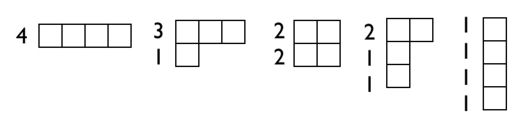
\includegraphics[width=0.6\linewidth]{Immagini/partitions of 4.png}
    \caption{Young diagrams corresponding to the partitions of four.}
    \label{fig: Young diagrams of the partitions of four}
\end{figure}

Permutations reorder the elements of a set $X$ with distinct elements. If one represents the elements of $X$ as letters of the alphabet and each ordering as a word, then each permutation is called an anagram. 
\begin{defn}[multiset]
    A multiset is defined as a set where an element $x_i$ can appear multiple times, specified by its multiplicity $m_i$.
\end{defn}
By this definition, the total number of elements of $X$ is $N = \sum_i m_i$. Different words formed by the elements are the different permutations of the multiset. A priori, $N$ elements can be reordered $N!$ times, but there are $m_1!$ to reorder the elements $x_1$, $m_2!$ ways to reorder the elements $x_2$, and so on. So, the total number of distinct re-orderings of the elements of $X$ is 
\begin{equation}
    \binom{N}{m_1,\dots,m_k} \equiv \frac{N!}{m_1!\cdots m_k!},
\end{equation}
where $k$ is the number of distinct elements of $X$ so that $N = \sum_{i=1}^k m_k$ is a partition of $N$. 

\section{Free groups and presentations}
\begin{defn}[free group]
    Let $G$ be a group and $X = {g_1,\dots,g_n}$ a subset of elements of $G$. If every element $g \in G\setminus\{e\}$ can be uniquely written as a product 
    \begin{equation}
        g = g_{j_1}^{i_1}\cdots g_{j_m}^{i_m},
    \end{equation}
    thus of elements $g_{j_k}$ taken only from the set $X$ with exponents $i_k \in \Z \setminus\{0\}$ such that no two adjacent elements are equal, $G$ is said to be a free group and $X$ is a free set of generators of $G$. 
\end{defn}
In analogy of what was said on multisets, the elements of $X$ are called ``letters'', so that an arbitrary product of letters $g = g_{j_1}^{i_1}\cdots g_{j_m}^{i_m}$ is called a ``word'' where $i_k \in \Z$. If the product satisfies the additional conditions of the previous definition, so $i_k \neq 0$ and $g_{j_i} \neq g_{j_{i+1}}$, the word is said to be a ``reduced word''. One can define a constraint called a ``relation'' and denoted with $r$ by setting a reduced word to be equal to the unit element by an equation
\begin{equation}
    r \equiv g_{j_1}^{i_1} \cdots g_{j_m}^{i_m} = e.
\end{equation}
In general, there can be several independent relations $r_i$ with $i \in \N$. 

A definition of a group $G$ now consists of the sets of generators $X = \{g_1,\dots,g_n\}$ and the complete list of independent relations $r_1,\dots,r_n$, so $G$ can be denoted with the notation
\begin{equation}
    G = \mybraket{g_1,\dots,g_n}{r_1,\dots,r_m},
\end{equation}
which is called a ``presentation'' of the group $G$. 
\begin{ex}
    Some examples of groups and their presentations are the followings:
    \begin{enumerate}
        \item Let $X = \{a\}$ and set $r \equiv a^n = e$. With this relation, the set $X$ generates the cyclic group $\Z_n = \{e,a,\dots,a^n\}$, whose representation is $\Z_n = \mybraket{a}{a^n}$. 
        \item The dihedral group $D_4$ is the group of symmetries of a square. Consider the operations $R$ as the rotation by $\pi/2$ and $f$ as the reflection with respect to the vertical axe passing through the midpoints of opposite sides. It is immediate to see the relations $r_1 \equiv R^4$ and $r_2 \equiv f^2$, but a bit less obvious is the relation $r_3 \equiv RfRf$. So, the dihedral group of order four can be denoted as $D_4 = \mybraket{R,f}{R^4,f^2,RfRf}$. More in general, the dihedral group $D_n$ describes the symmetries of regular polygons with $n$ sides, and can be denoted with the general presentation $D_n = \mybraket{R,f}{R^n,f^2,RfRf}$.
        \item The Pauli group is a finite group of order 16, consisting of the three Pauli matrices $\sigma^1$, $\sigma^2$, $\sigma^3$ and the identity matrix $\MI$ multiplied by the factors $\pm 1$ and $\pm i$, so $G_1$ is
        \begin{equation}
            G_1 = \{\pm\MI,\pm i\MI,\pm\sigma^1,\pm i\sigma^1,\pm\sigma^2,\pm i\sigma^2,\pm\sigma^3,\pm i\sigma^3\}.
        \end{equation}
        Recalling the relations $(\sigma^a)^2 = \MI$ and $\sigma^a\sigma^b = i\epsilon_{abc}\sigma^c$ the Pauli group can be defined through the presentation 
        \begin{equation}
            G_1 = \mybraket{\sigma^1,\sigma^2,\sigma^3}{(\sigma^a)^2,-i\epsilon_{abc}\sigma^a\sigma^b\sigma^c}.
        \end{equation}
    \end{enumerate}
\end{ex}

\section{Braids}
In general, a braid consists of strands which run forward and can pass under or over each other. In Physics, an important related situation is met when one considers word-lines of point particles moving in two dimensional spaces. The particle word-lines then form strands that become entangled, just like knitting strands. This phenomenon gives rise to exotic quantum statistics for quantum particles in two dimension\footnote{The reason why this is not true in three or more space dimension is that there the strands can be untangled} called ``anyons'', which are quasi-particles generalisation of fermions and bosons in three dimension. Here the convention is that the braid is drawn upright with braiding strands beginning from the top and proceeding downwards, the exact opposite of what shown in figure \ref{fig: anyons}. One can imagine that strands are like pieces of string and thus can be moved and deformed continuously. 
\begin{figure}[h]
    \centering
    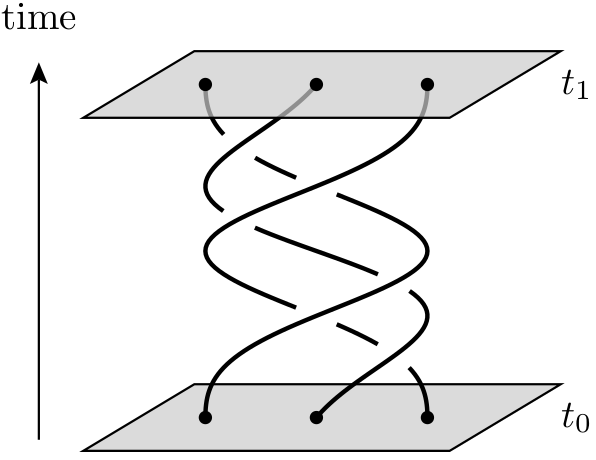
\includegraphics[width=0.4\linewidth]{Immagini/anyons.png}
    \caption{wordlines of three particles moving on a two dimensional plane.}
    \label{fig: anyons}
\end{figure}

In a braid of $n$ strands, the strands can be labelled by an index $i = 1,\dots,n$ running from left to right. A possible way to move strands in a braid is known as the ``Reidermeister move of the second type''\footnote{There exists also the Reidermeister move of the first type which is simply defined as untwisting a strand passing over itself.}, as shown in figure \ref{fig: RM of the II type}. 
\begin{figure}[h]
    \centering
    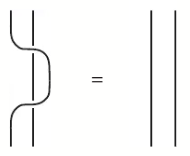
\includegraphics[width=0.3\linewidth]{Immagini/RM of the II type.png}
    \caption{the Reidermeister move of the second type.}
    \label{fig: RM of the II type}
\end{figure}

To form braids, another important basic operation, denoted as $\sigma_i$, consists in the moving of the $i$th strand over the $(i+1)$th strand, as shown in figure \ref{fig: sigma_i and sigma_i^-1 operations}. The inverse operation $\sigma_i^{-1}$ moves the $(i+1)$th strand over the $i$th strand, as shown again in picture \ref{fig: sigma_i and sigma_i^-1 operations}. A crucial rule to note is that after every operation, the strands are indexed again from left to right from 1 to $n$, and next operation is performed one the strands labelled according to the new indexing.
\begin{figure}[h]
    \centering
    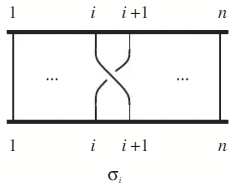
\includegraphics[width=0.35\linewidth]{Immagini/sigma_i operation.png}
    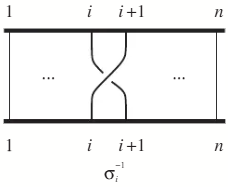
\includegraphics[width=0.335\linewidth]{Immagini/sigma_i^-1 operation.png}
    \caption{the basic operation. (i) $\sigma_i$ which moves $i$th over the $(i + 1)$th strand; (ii) $\sigma_i^{-1}$ which moves $(i + 1)$th over the $i$th strand.}
    \label{fig: sigma_i and sigma_i^-1 operations}
\end{figure}
To illustrate the indexing, consider the sequences of operations $\sigma_i\sigma_i^{-1}$ and $\sigma_i^2 = \sigma_i\sigma_i$. For the first one, after $\sigma_i$, the $i$th strand becomes the $(i+1)$th, and vice versa. With the new indexing, the next operation $\sigma_i^{-1}$ then acts in the opposite way of the first operation, the final result for $\sigma_i\sigma_i^{-1}$ coincides with the initial state, as shown in figure \ref{fig: sigma_i x sigma_i^-1 operation}, so the operation reduces to the trivial one $e$. The same thing happens for $\sigma_i^{-1}\sigma_i$. 
\begin{figure}[h]
    \centering
    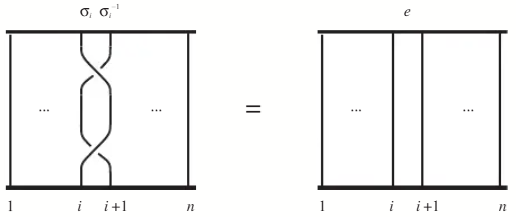
\includegraphics[width=0.7\linewidth]{Immagini/sigma_i x sigma_i^-1 operation.png}
    \caption{equivalence between the identity element $e$ and the sequence of operations $\sigma_i\sigma_i^{-1}$.}
    \label{fig: sigma_i x sigma_i^-1 operation}
\end{figure}

By the same rules, the operation $\sigma_i\sigma_i$ does not reduce to $e$, instead the strands become tangled with a non-trivial final result, as shown in figure \ref{fig: sigma_i^2 operation}. 
\begin{figure}[h]
    \centering
    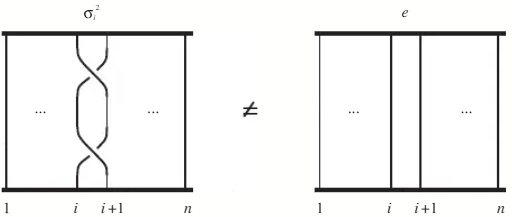
\includegraphics[width=0.7\linewidth]{Immagini/sigma_i^2 operation.png}
    \caption{inequivalence between the identity element $e$ and the sequence of operations $\sigma_i^2$.}
    \label{fig: sigma_i^2 operation}
\end{figure}

After these examples, one can generalise the discussion by moving to more general constructions. For a braid of $n$ strands, the basic operations $\sigma_1,\dots,\sigma_{n-1}$, that can be thought of as the letters of a set $X_{n-1}$, thus, each word is
\begin{equation}
\label{eq: definition of a generic braid}
     \sigma = \sigma_{j_1}^{i_1}\cdots\sigma_{j_m}^{i_m},\quad i_m \in \Z,
\end{equation}
represents a braid. As before, when drawing the braid, one starts from the top, reads the letters of the word from left to right and performs the corresponding operation on the strands, continuing the drawing downwards. The inverse of a generic braid defined in \eqref{eq: definition of a generic braid} is obtained as the product of the inverse operations in the opposite order
\begin{equation}
    \sigma^{-1} = \sigma_{j_m}^{-im}\cdots \sigma_{j_1}^{-i_1}.
\end{equation}
The group generated by $X_{n-1}$ for $n > 2$ is not a free group. There are relations among the generators, because one can move and deform the strands continuously. One relation is due to the fact that the operations of braiding strands that are sufficiently apart from each other are independent operations, so their generators commute
\begin{equation}
\label{eq: commutation relation between braid generators}
    \sigma_i\sigma_j = \sigma_j\sigma_i,\quad |i - j| \ge 2.
\end{equation}
A less obvious relation is the Reidermeister move of the third type
\begin{equation}
\label{eq: Reidermeister move of the III type}
    \sigma_i\sigma_{i+1}\sigma_i = \sigma_{i+1}\sigma_i\sigma_{i+1}.
\end{equation}
It turns out that the diagram in figure \ref{fig: Yang-Baxter relation} also appears in the context of exactly solvable problems in statistical mechanics and quantum field theories, where it is related to a Yang-Baxter relation. This is not an accident, since the conditions that determine the integrability of those models have a connection with the properties of braids. 
\begin{figure}[h]
    \centering
    
\includegraphics[width=0.4\linewidth]{Immagini/Yang-Baxter relation.png}
    \caption{diagram showing the equivalence $\sigma_i\sigma_{i + 1}\sigma_i = \sigma_{i + 1}\sigma_i\sigma_{i + 1}$, namely the Reidermeister move of the third type.}
    \label{fig: Yang-Baxter relation}
\end{figure}

One can show that the relations \eqref{eq: commutation relation between braid generators} and \eqref{eq: Reidermeister move of the III type} are the only relations between the generators $\sigma_i$. This leads up to define the braid group of $n$ strands $B_n$ by its presentation
\begin{equation}
    B_n = \mybraket{\sigma_1,\dots,\sigma_n}{\sigma_i\sigma_j = \sigma_j\sigma_i,\,\sigma_i\sigma_{i+1}\sigma_i = \sigma_{i+1}\sigma_i\sigma_{i+1}},
\end{equation}
where $|i - j| \ge 2$ in the first relation and $1 \le i \le n - 2$ in the second one. In conclusion, some properties of braid groups are the following:
\begin{enumerate}
    \item $B_1$ is the trivial group $\Z_1 = \{e\}$;
    \item $B_2 \simeq (\Z_2,+)$ so it is an Abelian group;
    \item $B_3$ is non-Abelian;
    \item the braid groups form a nested sequence of subgroups $B_n \subset B_{n + 1}$ for every positive real natural number $n$.
\end{enumerate}

\section{Continuous groups}
Continuous groups are groups having an infinite and uncountable number of elements. Since the order of a continuous group is not a meaningful concept, the ``size'' of a continuous group is instead characterized in terms of its dimension.
\begin{defn}[dimension]
    The dimension of a continuos group $G$ denoted with $\dim{G}$ is the minimum number of real parameters needed to uniquely identify its elements.
\end{defn}
The real parameters identifying an element of a continuos group are called its ``coordinates'', where each one may take values within the whole $\R$, or within a real interval. The definition of a group dimension is distinct from, and more general, the definition of dimension of a vector space. Indeed, continuous groups may, but not necessarily have to, be realized in terms of linear vector spaces. As will discussed later, given the product of two elements $g \cdot g' = g''$, where $g,g' \in G$, the coordinates of $g''$ must be continuous functions of the coordinates $g$ and $g'$. This means that the set of coordinates parametrizing a group form a manifold, called the ``group manifold''. The most interesting continuous groups are Lie groups.
\begin{defn}[Lie group]
    A Lie group is a continuous group whose group manifold is differentiable, so it is possible to take smooth derivatives of the group elements with respect to the coordinates.
\end{defn}
Particularly interesting Lie groups are those defined from certain sets of matrices, with the usual matrix multiplication law as the group composition operation.
\paragraph{$\bm{GL(n,\R)}$ group.} The group of general linear transformations with real coefficients denoted as $GL(n, \R)$ is defined as the subset of matrices in $\R^{n,n}$ having a non-vanishing determinant, with the matrix product as the group multiplication:
    \begin{equation}
        GL(n, \R) = \{ A \in \R^{n,n} : \det A \neq 0 \}.
    \end{equation}
    The identity matrix of size $n \times n$ is the unit element of the group, and the existence of the inverse of any element of $GL(n, \R)$ is guaranteed by the condition that the determinant is different from zero. Note that the determinant of a matrix is a continuous function of its entries. The dimension of $GL(n, \R)$ is $\dim GL(n, \R) = n^2$, like that of $\R^{n,n}$. Note that the constraint that the determinant of the elements of $GL(n, \R)$ is different from zero does not reduce the number of independent real parameters of $GL(n, \R)$. While $GL(n, \R)$ and $\R^{n,n}$ have the same dimension, their group manifolds have a different global structure. In particular, in contrast to $\R^{n,n}$, for which the matrix entries are a set of suitable coordinates, in $GL(n, \R)$ the condition $\det A \neq 0$ for a generic group element $A$ implies that the coordinates parametrizing the group elements cannot take arbitrary values in $\R^{n,n}$, but rather in $\R^{n,n}$ with the exclusion of the hypersurface on which the matrix determinant vanishes (this hypersurface is a set of measure zero in $\R^{n,n}$). Thus the group manifold of $GL(n, \R)$ is divided into two disconnected components (in which the determinant of a generic element is either positive or negative).

\paragraph{$\bm{GL(n,\C)}$ group.} The group of general linear transformations can be generalized, by allowing the matrix elements to take values in the complex field; this leads to the group
    \begin{equation}
        GL(n, \mathbb{C}) = \{ A \in\C^{n,n}) : \det A \neq 0 \},
    \end{equation}
    again with matrix product as the group multiplication. As for the group $GL(n, \R)$, the unit element is the identity matrix of size $n \times n$, and the existence of the inverse of any element of the group is guaranteed by the fact that the determinant is non-vanishing. Since each of the $n^2$ entries of a generic matrix $A \in GL(n, \mathbb{C})$ is a complex number, which can be parametrized by two real coordinates, and since the $\det A \neq 0$ constraint does not reduce the number of independent parameters, the dimension of $GL(n, \mathbb{C})$ is $2n^2$. Finally, note that $GL(n, \R)$ is a proper subgroup of $GL(n, \mathbb{C})$. The group $GL(n, \mathbb{C})$ and its subgroups are called matrix Lie groups.

\paragraph{$\bm{SL(n,\R)}$ group.} The set of special linear transformations of degree $n$ with real coefficients is denoted as $SL(n, \R)$ and is defined as
    \begin{equation}
        SL(n, \R) = \{ A \in \R^{n,n} : \det A = 1 \}.
    \end{equation}
    Note that, since $\det A = 1$ is a special case of $\det A \neq 0$, $SL(n, \R)$ is a subset of $GL(n, \R)$. Taking the matrix product as the composition law, and observing that the product of two matrices with determinant $1$ also has determinant $1$, that the inverse of any matrix of determinant $1$ also has determinant $1$, and that the determinant of the identity matrix is $1$, too, it follows that $SL(n, \R)$ is a proper subgroup of $GL(n, \R)$. The dimension of $SL(n, \R)$ is $n^2 - 1$: the condition that the determinant of each element equals $1$ is expressed as an equation, that reduces the number of independent coordinates from $n^2$ down to $n^2 - 1$.

\paragraph{$\bm{O(n,\R)}$ group.} The orthogonal group of degree $n$ is defined as the group of real matrices (orthogonal matrices) whose inverse coincides with their transpose. For a given matrix $A$, the latter is defined as the matrix obtained from $A$ by interchanging its rows with its columns, $(A^T)_{ab} = A_{ba}$:
    \begin{equation}
        O(n, \R) = \{ A \in GL(n, \R) : A^T A = A A^T = \MI \},
    \end{equation}
    where $\MI$ is the identity matrix of size $n \times n$. It is easy to prove that $O(n, \R)$ (with the matrix product as the group multiplication) is a proper subgroup of $GL(n, \R)$, since:
    \begin{enumerate}
        \item the product of two elements of $O(n, \R)$, $A$ and $B$, is also an orthogonal matrix:
        \begin{equation}
            (AB)^T (AB) = B^T A^T A B = B^T B = \MI;
        \end{equation}
        \item the unit element for the matrix product is the identity matrix, which is an orthogonal matrix $(\MI^T \MI = \MI)$;
        \item the inverse of a generic orthogonal matrix $A$ is also orthogonal:
        \begin{equation}
            (A^{-1})^T A^{-1} = (A A^T)^{-1} = \MI^{-1} = \MI.
        \end{equation}
    \end{enumerate}
    Orthogonal matrices can be seen as linear transformations acting on the $n$-dimensional real vector space $\R^n$ and preserve the modulus of vectors in $\R^n$. Indeed, the modulus of a vector $\vv \in \R^n$ is given by $\sqrt{\sum_{a=1}^n v_a^2} = \sqrt{\vv^T \vv}$. Upon a transformation $A \in O(n, \R)$, the vector $\vv$ gets mapped to $A\vv$, whose modulus is $\sqrt{(A\vv)^T (A\vv)} = \sqrt{\vv^T A^T A \vv} = \sqrt{\vv^T \vv}$, namely it is left invariant. As a consequence, the orthogonal group can be interpreted as a group of rotations and reflections in $\R^n$. To determine the dimension of $O(n, \R)$, note that each element is expressed by a matrix with $n^2$ real entries, but they are not all independent, because the orthogonality condition restricts the number of independent coordinates. In particular, the requirement that $A^T A = \MI$ implies that each diagonal entry of $A^T A$ must be equal to $1$; this imposes $n$ equations. In addition, all of the entries above the diagonal must vanish, and this gives further $n(n-1)/2$ independent equations. If the entries above the diagonal vanish, then so do those below the diagonal, because $A^T A$ is a symmetric matrix. The constraints imposed by the $A A^T = \MI$ condition equivalent. Hence, the orthogonality constraint reduces the number of independent real parameters down to $n^2 - n - n(n-1)/2 = n(n-1)/2$. Finally, note that the orthogonality condition (and the fact that the determinant of a matrix and that of its transpose are equal) also implies that the determinant of any element of $O(n, \R)$ is either $1$ or $-1$, because $\det(A^T A) = \det \MI$ implies $(\det A)^2 = 1$, hence $\det A = \pm 1$. The subset of $O(n, \R)$ including the matrices of determinant $1$ is the special orthogonal group of degree $n$:
    \begin{equation}
        SO(n, \R) = \{ A \in GL(n, \R) : A^T A = A A^T = \MI,\ \det A = 1 \}.
    \end{equation}
    The special orthogonal group of degree $n$ is a proper subgroup of $O(n, \R)$ and its dimension is $\dim SO(n, \R) = n(n-1)/2$, like $O(n, \R)$ (because the determinant of elements of $O(n, \R)$ can only take values $\pm 1$, hence the condition that the determinant equals $1$ for $SO(n, \R)$ elements does not reduce the number of independent real coordinates). $SO(n, \R)$ can be interpreted as the subgroup of $O(n, \R)$ which preserves the orientation of a basis of vectors in $\R^n$. So, for example, acting with a matrix of $SO(3, \R)$ on the vectors of a right-handed orthonormal basis of $\R^3$ results into a rotated basis of vectors, which is still right-handed. Note that, by contrast, the subset of $O(n, \R)$ including the matrices with determinant $-1$ is not a subgroup (in fact, it is not even a magma, since $\det A = \det B = -1$ implies $\det(AB) = 1$). Often the orthogonal groups and their special subgroups are denoted as $O(n)$ and $SO(n)$.

\paragraph{$\bm{U(n)}$ group.} The generalization of the orthogonal group of degree $n$ to the complex field is the unitary group of degree $n$, defined as
    \begin{equation}
        U(n) = \{ A \in GL(n, \C) : A^\dg A = A A^\dg = \MI \},
    \end{equation}
    where $A^\dg = (A^*)^T = (A^T)^*$ is the conjugate transpose of $A$: $(A^\dg)_{ij} = (A_{ji})^*,$ with $*$ denoting complex conjugation. Note that $(AB)^\dg = B^\dg A^\dg$. These matrices preserve the modulus of complex vectors $\vv \in \C^n$, defined as $\sqrt{\sum_{a=1}^n z_a^* z_a} = \sqrt{\vv^\dg \vv}$. A generic element $A \in U(n)$ maps a vector $\vv$ to $A\vv$, whose modulus is $\sqrt{(A\vv)^\dg (A\vv)} = \sqrt{\vv^\dg A^\dg A \vv} = \sqrt{\vv^\dg \vv}$, namely is left invariant by the action of $A$. Hence unitary matrices can be interpreted as ``rotations'' in $\C^n$. (More generally, a linear map $A : V \to W$ between two vector spaces $V$ and $W$ that preserves the lengths of vectors is called an isometry.) $U(n)$ is a proper subgroup of $GL(n, \C)$. One can show that $\dim U(n) = n^2$: Starting from the dimension of $GL(n, \C)$, which is $2n^2$ (where the factor $2$ accounts for the fact that each matrix element has a real and an imaginary part), the dimension of $U(n)$ can be obtained by subtracting from it the number of independent constraints that the $U(n)$ matrix entries must obey. From the requirement that $A^\dg A = \MI$ follows, first of all, that each diagonal element of $A^\dg A$ must be equal to $1$:
    \begin{equation}
    \label{eq: unitarity condition of U(n) group I}
        (A^\dg A)_{ii} = \sum_{k=1}^n A^\dg_{ik} A_{ki} = (\MI)_{ii} = \delta_{ii} = 1, \quad \forall i : 1 \le i \le n.
    \end{equation}
    Using the fact that $A^\dg_{ik} = A^*_{ki}$, \eqref{eq: unitarity condition of U(n) group I} can be rewritten as
    \begin{equation}
    \label{eq: unitarity condition of U(n) group II}
        \sum_{k=1}^n A^*_{ki} A_{ki} = \sum_{k=1}^n |A_{ki}|^2 = 1, \quad \forall i : 1 \le i \le n.
    \end{equation}
    Equation \eqref{eq: unitarity condition of U(n) group II} corresponds to $n$ constraints (not $2n$, because a sum of squared moduli of complex numbers is necessarily a real, non-negative number, namely the imaginary part of each sum is already necessarily zero, without imposing any constraint on it). Conversely, for the $n(n-1)/2$ elements above the diagonal of the $A^\dg A$ matrix, the conditions
    \begin{equation}
    \label{eq: above diagonal elements condition of U(n) group}
        (A^\dg A)_{ij} = \sum_{k=1}^{n} A_{ik}^\dg A_{kj} = 0, \quad 1 \le i < j \le n,
    \end{equation}
    enforce the vanishing of the real and of the imaginary part, and thus correspond to two independent constraints for each element. Finally, the constraints on the remaining $n(n-1)/2$ elements below the diagonal of the $A^\dg A$ turn out to be equivalent to those expressed by \eqref{eq: above diagonal elements condition of U(n) group}. Also, one can check that the same constraints arise if one requires $A A^\dg = \MI_n$. To conclude, note that the dimension of the unitary group of degree $n$ is given by $\dim U(n) = 2n^2 - n - 2\, n(n-1)/2 = n^2$. Note that, according to the definition \eqref{eq: unitarity condition of U(n) group I}, $U(1) = \{ a \in \C : a^* a = 1 \}$, so the group manifold of $U(1)$ can be identified with the circle of unit radius on the complex plane. The subset of $U(n)$ containing matrices of determinant equal to $1$ constitutes the special unitary group of degree $n$:
    \begin{equation}
        SU(n) = \{ A \in U(n), \det A = 1 \}.
    \end{equation}
    This is a proper subgroup of $U(n)$, and its dimension can be computed by noting that, in addition to the constraints that every $U(n)$ matrix must satisfy, the requirement $\det A = 1$ imposes one additional condition (not two, because from $A^\dg A = \MI_n$, which holds for every unitary matrix $A$, and from the property that $\det A^\dg = (\det A)^*$, already follows that $\det(A^\dg A) = \det(A^\dg)\det A = (\det A)^* \det A = |\det A|^2 = \det \MI_n = 1$, namely the real and imaginary parts of $\det A$ cannot be arbitrary numbers, since they already satisfy the constraint that $|\det A| = 1$). Thus $\dim SU(n) = (\dim U(n)) - 1 = n^2 - 1$. The subset of $\R^{2n,2n}$ containing the matrices $M$, called ``symplectic matrices,'' that satisfy the property
    \begin{equation}
        M^T \Omega M = \Omega, \quad \Omega =
        \begin{pmatrix}
        0_n & \MI_n \\
        -\MI_n & 0_n
        \end{pmatrix}.
    \end{equation}

\section{Groups acting on a set}
\begin{defn}[left-action]
    Given a group $G$ and a set $X$, a left-action of $G$ on $X$ is a homomorphism
    \begin{equation}
        L : G \to \Perm{X},\quad g \mapsto L_g.
    \end{equation}
\end{defn}
Since a left-action is a group homomorphism, it preserves the group multiplication 
\begin{equation}
    \forall g_1,g_2 \in G,\,\forall x \in X : L_{g_2}(L_{g_1}(x)) = L_{g_2 \cdot g_1}(x).
\end{equation}
\begin{defn}[left group-space]
    Given a group $G$, a set $X$ is called a left group-space of $G$, or a left $G$-space, if there exists a left-action of $G$ on $X$.
\end{defn}
Similarly, one can define a right-action and a right group-space.
\begin{defn}[right-action]
    Given a group $G$ and a set $X$, a right-action of $G$ on $X$ is a homomorphism
    \begin{equation}
        R : G \to \Perm{X},\quad g \mapsto R_g,
    \end{equation}
    such that it preserves the group multiplication
    \begin{equation}
        \forall g_1,g_2 \in G,\,\forall x \in X : R_{g_2}(R_{g_1}(x)) = R_{g_2 \cdot g_1}(x).
    \end{equation}
\end{defn}
\begin{defn}[right group-space]
    Given a group $G$, a set $X$ is called a right group-space of $G$, or a right $G$-space, if there exists a right-action of $G$ on $X$.
\end{defn}
Given a group $G$, two left $G$-spaces $X$ and $X'$ can be identified, if there is a bijection $i : X \to X'$ such that, for any $g \in G$ and for any $x \in X$, one has $i(L_g(x)) = L_g'(i(x))$, where $L$ and $L'$ are the left-actions of $G$ on $X$ and on $X'$, respectively. An analogous definition can be made for right $G$-spaces and right-actions. 
\begin{defn}[orbit]
    Given a left $G$-space $X$ of a group $G$, the orbit of a point $x \in X$ under the left-action $L$ of $G$ on $X$ is the set
    \begin{equation}
        O_x = \{g \in G\ : L_g(x) \}.
    \end{equation}
\end{defn}
In other words, the orbit of a point $x \in X$ is the subset of $X$ containing all points that can be reached from $x$ by acting on it with the left-action of some element of $G$. Given a group $G$, a left-action of $G$ on $X$ is said to be ``transitive'' when all elements of $X$ belong to the same orbit, in other words $X/G$ contains only one element. In practice, a left-action $L$ of a group $G$ on a set $X$ is transitive when for any $x \in X$ and any $y \in Y$, there exists an element $g \in G$, such that $y = L_g(x)$, so a left-action is transitive if it connects evey pair of elements in $X$. 
\begin{defn}[homogeneous space]
    A set $X$ is said to be a homogeneous space under the action of $G$, when the action of $G$ on $X$ is transitive.
\end{defn}
\begin{ex}
    Let $G = \Z_2 = \{e,a\}$ and $X = \R$. Consider the left-action $L$ such that $L_e(x) = x$ and $L_a(x) = -x$. The orbit of a generic point $x \in X$ contains either two distinct elements $O_x = \{x,-x\}$ if $x \neq 0$ or just $x$ itself if $x = 0$. Hence, two generic elements $x,y \in X$ belong to the same orbit only if $x = \pm y$. The action is not transitive, because $X/G$ contains infinitely many orbits, namely one for each non-negative real number.
\end{ex}
\begin{defn}[isotropy group]
    Given a group $G$, a left $G$-space $X$, and an element $x \in X$, the isotropy group of $x$ is the subgroup of $G$ containing all elements that leave $x$ invariant
    \begin{equation}
        G_x = \{g \in G : L_g(x) = x\}.
    \end{equation}
\end{defn}
For some points $x$ it may turn out that $G_x = G$, so $L_g(x) = x$ for any $g \in G$; in this case $x$ is said to be a ``fixed point'' under the action of $G$. One can also be interested in the converse problem, that of finding all the points that are left invariant by the action of a given element $g$ of a group $G$. 
\begin{defn}[isotropy set]
    Let $g$ be an element of a group $G$ acting on a set $X$, the set of points left invariant by the left-action of $g$ is defined as
    \begin{equation}
        X^g = \{x \in X : L_g(x) = x\}.
    \end{equation}
\end{defn}
Note that for the unit element $e$ one have $X^e = X$ since $e$ is always represented by the identity map. A particularly interesting case of group-space is the group itself $X = G$. The simplest left and right-actions are simply the ``translations'', so the actions defined by multiplication by a group element on the left and on the right. The left translation of a group $G$ is the group homomorphism $L : G \to \Perm{G}$, with $g \mapsto L_g$, defined $L_g(g') = g\cdot g'$ for any $g' \in G$. Similarly, the right translation is the group homomorphism $R : G \to \Perm{G}$, with $g \mapsto R_g$, defined as $R_g(g') = g'\cdot g$ for any $g' \in G$. Note that the left, or right, translation is always a transitive action: every group element belongs to the orbit of the unit element $e$, since $L_g(e) = g \cdot e = g$, or $R_g(e) = e \cdot g = g$, in other words $O_e = G$. A more interesting way to define the group action on itself is by conjugation.
\begin{defn}[conjugation]
    The conjugation of a group $G$ is the group homomorphism $L : G \to \Perm{G}$, with $g \mapsto L_g$, defined as
    \begin{equation}
        L_g(g') = g\cdot g' \cdot g^{-1},\quad \forall g' \in G.
    \end{equation}
\end{defn}
\begin{defn}[conjugacy class]
    A conjugacy class of an element of a group $G$ is defined as its orbit under conjugation.
\end{defn}
In other words, the conjugacy class of a generic element $g \in G$ is the subset of $G$ containing all elements $g$ that can be written in the form $g' = x \cdot g \cdot x^{-1}$ for some $x \in G$. Then $g$ and $g'$ are said to be ``conjugate'', and $x$ is called the ``conjugating element''. In general, conjugation is not a transitive action. It is also interesting to consider the action of a subgroup $H \subset G$ on $G$. In particular, the right-action of $H$ on $G$ defined by translation, $R_h(g) = g \cdot h$, is not necessarily transitive if $H$ is a proper subgroup. 
\begin{defn}[left coset]
    Given a group $G$ and a subgroup $H \subset G$, the left coset associated with an element $g \in G$ is the orbit of $g$ under right translation by elements of $H$, so the set 
    \begin{equation}
        gH = \{g' \in G : \exists h \in H : g' = g \cdot h\}.
    \end{equation}
\end{defn}
\begin{defn}[right coset]
    Given a group $G$ and a subgroup $H \subset G$, the right coset associated with an element $g \in G$ is the orbit of $g$ under left translation by elements of $H$, so the set 
    \begin{equation}
        Hg = \{g' \in G : \exists h \in H : g' = h \cdot g\}.
    \end{equation}
\end{defn}
The set of left cosets forms the quotient space $G/H = \{gH : g \in G\}$, while the set of right cosets forms the quotient space $H\setminus G = \{Hg : g \in G\}$. Obviously, when $G$ is an Abelian, left and the right cosets coincide. Note that, if two elements $g,g' \in G$ can be obtained from each other via right translation by an element of the subgroup, so $g' = g\cdot h$ with $h \in H$, then their left and right cosets coincide $gH = Hg$. The inverse is also true: if the left cosets of two elements $g,g'\in G$ coincide, the $g^{-1}\cdot g' \in H$, so it exists a unique $h \in H$ such that $g' = g\cdot h$. Finally, one can prove that the elements of each coset can be put in a one-to-one correspondence with the elements of $H$ itself. 
\begin{proof}
    For a given $g \in G$, the mapping $f_g : H \to gH$, with $h \mapsto g\cdot h$, is surjective, by definition of $gH$. It also is injective, because multiplying $g\cdot h_1 = g\cdot h_2$ by $g^{-1}$ on the left if follows that $h_1 = h_2$. Thus, $f_g$ is a bijection, so it is a one-to-one correspondence between $H$ and the generic coset $gH$.
\end{proof}
In particular, if $H$ is a finite subgroup, then the order of all cosets must equal $|H|$. This leads to the following theorem. 
\begin{teo}[Lagrange's theorem]
\label{teo: Lagrange's theorem}
    The order $|H|$ of any subgroup $H$ of a finite group $G$ must be a divisor of $|G|$.
\end{teo}
\begin{proof}
    Under the right-action of $H$, the group $G$ is partitioned into mutually disjoint orbits $gH$, each having the same order as $H$. Hence, $|G| = n|H|$ for some $n \in \N$.
\end{proof}
\begin{corl}
    If $p$ is a prime number, then $\Z_p$ is the only subgroup of order $p$.
\end{corl}
\begin{proof}
    Consider a generic finite group $G$ of order $p$, and let $g$ be an element of $G$ different from the unit element $e$ of $G$. Let $m$ denote the order of $g$; since $g \neq e$, it follows that $m > 1$. Then $H = \{e,g,\dots,g^{m - 1}\} \simeq \Z_m$ is a subgroup of $G$. Lagrange's theorem implies $p = nm$, but since $p$ is prime and $m  > 1$, then necessarily $n = 1$ and $p = m$, thus $|G| = |H|$. Then $G$ coincides with $H$, which is isomorphic to $\Z_p$. Thus any finite group of order $p$ is isomorphic to $Z_p$, which is the only abstract group of order $p$.
\end{proof}
Note that the quotient space $G/H$ is a $G$-space, if one defines the left-action $L : G \to \Perm{G/H}$, with $g \mapsto L_g$, as
\begin{equation}
    L_g(g'H) = gg'H.
\end{equation}
Note that any two arbitrary elements of $G/H$ always belong to the same orbit defined by $L$, because $y = g_2g_1^{-1} \in G$, and $L_yg_1H = g_2g_1^{-1}g_1H = g_2H$, thus the action is transitive. The inverse statement is also true.
\begin{teo}
\label{teo: correspondence quotient-set}
    Every group $G$ acting transitively on a set $X$ admits a subgroup $H$, such that the quotient space $G/H$ is in one-to-one correspondence with $X$.
\end{teo}
\begin{proof}
    For a given $x \in X$, consider its isotropy group $G_x$ as a subgroup $H$. Consider the map $i : G/H \to X$ defined as $i(gH) = L_g(x)$. Note that $i$ is well defined, so $i(gH)$ does not depend on the representative $(g)$ chosen in $gH$, because the definition of $gH$ implies that for any other representative $g' \in gH$ there exists ah $h \in H$ such that $g = g'h$. Thus $L_g(x) = L_{g'h}(x)$, and, since $L$ is a group homomorphism, this implies $L_g(x) = L_{g'}(L_h(x)$. But $L_h(x) = x$, because $h \in H$ and $H$ is the isotropy group of $x$. As a consequence, $L_g(x) = L_{g'}(x)$. Moreover, $i$ is injective, because $i(gH) = i(g'H)$ means $L_g(x) = L_{g'}(x)$, which implies $x = L_{g^{-1}g'}(x)$, which means that $L_{g^{-1}g'}$ leaves $x$ invariant, so $g^{-1}g' \in H$. This means that $g' = gh$, thus the cosets $gH$ and $g'H$ are equal. Finally, $i$ is also surjective; since $G$ acts transitively, for any $x' \in X$ there exists a $g \in G$ such that $x' = L_g(x)$. But the right-hand side of the latter equation equals $i(gH)$, hence for any $x' \in X$ there exists a $g \in G$ such that $x' = i(gH)$.Thus there exists a bijective correspondence $i$ between $X$ and $G/H$. 
\end{proof}
\begin{corl}
\label{corl: correspondence quotient-set}
    The orbit of a point $x \in X$ can be identified with $G/G_x$.
\end{corl}
\begin{proof}
    Since $G$ acts transitively on its orbit, the statement of the corollary is a consequence of the previous theorem.
\end{proof}
Thus the orbits are determined by the subgroups of $G$; in other words, the action of $G$ on $X$ is determined by its subgroup structure.
\begin{ex}
    Consider the left-action of $G = SO(3,\R)$ on $\R^3$. The orbits are the spheres $|x^2| = x_1^2 + x_2^2 + x_3^2 = r^2$, which can be identified with the $S^2$ sphere for any $r > 0$. Given the point $x = (0,0,r)$ on each orbit $r > 0$, its isotropy group is
    \begin{equation}
        G_x = \bigg\{
        \begin{pmatrix}
            A_{2 \times 2} & 0 \\
            0 & 1 
        \end{pmatrix} : A_{2 \times 2} \in SO(2,\R)
        \bigg\} \simeq SO(2,\R).
    \end{equation}
    By theorem \ref{teo: correspondence quotient-set} and its corollary \ref{corl: correspondence quotient-set}, it follows that $SO(3,\R)/SO(2,\R) \simeq S^2$.
\end{ex}

If $G$ is a finite group acting on a finite set $X$, by a similar argument as the proof of Lagrange's theorem the following one is derived.
\begin{teo}[orbit stabilizer]
    If $G$ is a finite group acting on a finite set $X$, then it is true that
    \begin{equation}
        |G| = |G_x|\cdot |O_x|,\quad \forall x \in X.   
    \end{equation}
\end{teo}
The following lemma is sometimes useful in combinatorial problems.
\begin{lem}[Burnside's lemma]
    Let $G$ be a finite group acting on a finite set $X$. The number of orbits $|X/G|$ is given by
    \begin{equation}
        |X/G| = \frac{1}{|G|}\sum_{g \in G}|X^g|.
    \end{equation}
\end{lem}
Since the quotient space $G/H$ is constructed out of a group and its subgroup, it is natural to ask if it can also be a group. The first guess for a multiplication law would be $(g_1H)(g_2H) = g_1g_2H$. This definition would be meaningful if the right-hand side were independent of the labelling of the cosets, but this is not always the case; the first factor on the left-hand side is such that $g_1H = g_2H$ for any $h \in H$, so one could replace $g_1$ with $g_1h$; however, on the right-hand side it is not necessarily true that $g_1g_2H$ and $g_1hg_2H$ coincide. To endow $G/H$ with a meaningful group multiplication, it is convenient to require $H$ to be a normal subgroup. If that is the case, then the quotient space $G/H$ can be endowed with group structure by defining the group multiplication as
\begin{equation}
\label{eq: group multiplication of G/H}
    (g_1H)(g_2H) = g_1g_2H,\quad \forall g_1H,g_2H \in G/H.
\end{equation}
The fact that $H$ is a normal subgroup makes the right-hand side uniquely defined, in the sense that it makes the definition of the group multiplication meaningful: on the left-hand side, $g_1$ and $g_2$ are defined only up to right translations by elements of $H$, so that the right-hand side of the equation above could be replaced by $g_1h_1g_2h_2H$. This is obviously equal to $g_1h_1g_2H$, so the ambiguity in the definition of $g_2$ is not a problem. If $H$ is a normal subgroup, then there exists an $h \in H$ such that $h_1g_2 = g_2h$; then $g_1h_1g_2H = g_1g_2hH$ which in turn is equal to $g_1g_2H$, so the right-hand side of \eqref{eq: group multiplication of G/H} is unaffected by the ambiguity in the definition of $g_1$ and $g_2$. It is trivial to show that this definition of group multiplication in $G/H$ satisfies associativity that it admits a unit element and that every element $gH \in G/H$ has $g^{-1}H$ as its inverse. With the multiplication defined by \eqref{eq: group multiplication of G/H}, the quotient space $G/H$ becomes a group called the ``quotient group''. Note that, by Lagrange's theorem \ref{teo: Lagrange's theorem}, if $G$ is a finite group then the order of $G/H$, or of $H \setminus G$, is $|G|/|H|$.
\begin{ex}
    Consider the cyclic group $\Z_{2N} = \{e, a, a^2, \ldots, a^{2N-1}\}$, for a generic $N \in \N_0$ and its subset $H = \{e, a^2, a^4, \ldots, a^{2N-2}\}$. It is easy to prove that $H$ is a subgroup of $\Z_{2N}$. Since cyclic groups are Abelian, $H$ is normal. The two cosets are $eH = a^2H = \cdots = a^{2N-2}H$ and $aH = \{a, a^3, a^5, \ldots, a^{2N-1}\} = a^3H = \cdots = a^{2N-1}H$. Since $(eH)^2 = e^2H = eH$, while $(aH)(eH) = aeH = aH$, $(eH)(aH) = eaH = aH$, and $(aH)^2 = a^2H = eH$, the quotient group $\Z_{2N}/H$ is isomorphic to $\Z_2$.
\end{ex}
\begin{ex}
    Let $G = SU(2)$ and $H = \{\MI_2, -\MI_2\} \simeq \Z_2$. Obviously $A \in SU(2)$ satisfies the property $A(\pm \MI_2) = \pm \MI_2 A$, hence $H$ is a normal subgroup. Thus the quotient space $SU(2)/\Z_2$ is a group; in particular, it turns out to be isomorphic to $SO(3, \R)$.
\end{ex}
\begin{defn}[centre]
    The centre of a group $G$, denoted with $\Z(G)$, is the set of elements that commute with every element of $G$
    \begin{equation}
        \Z(G) := \{z \in G : \forall g \in G,\,z \cdot g = g \cdot z\}.
    \end{equation}
\end{defn}
One can prove that the centre of a group is a subgroup and obviously it is Abelian. By the definition of centre definition, a group $G$ is Abelian if and only if $\Z(G) = G$. Moreover, the centre is also normal; hence, the quotient space $G/\Z(G)$ is always a group. If the centre is trivial $\Z(G) = \{e\}$ then $G/\Z(G) \simeq G$. On the other hand, the centres of some non-Abelian groups are as follows:
\begin{enumerate}
    \item $G = S_3$ has a trivial centre: $\Z(G) = \{e\}$;
    \item $G = D_4$ has centre $\Z(G) = \{e, a^2\} \simeq \Z_2$; the quotient group $G/\Z(G)$ is isomorphic to the Klein four-group $\Z_2 \times \Z_2$;
    \item $G = Q_8$ has centre $\Z(G) = \{e, -e\} \simeq \Z_2$; the quotient group $G/\Z(G)$ is isomorphic to the Klein four-group $Z_2 \times Z_2$;
    \item $G = SO(2k+1, \R)$, with $k \geq 1$, has a trivial centre $\Z(G) = \{e\}$;
    \item $G = SO(2k, \R)$, with $k \geq 2$, has centre $\Z(G) = \{e, -e\} \simeq Z_2$;
    \item $G = U(N)$ has centre $\Z(G) = \{\exp(i\theta),\, \theta \in [0,2\pi)\} \simeq U(1)$;
    \item $G = SU(N)$ has centre $\Z(G) = \{\exp(2k\pi i/N)\,\MI_N,$ for $k \in [0,N-1]\}$, which is isomorphic to $\Z_N$;
    \item $G = Sp(2N, \R)$ has centre $\Z(G) = \Z_2$;
    \item $G = \G_2$ has a trivial centre $\Z(G) = \{e\}$;
    \item $G = \F_4$ has a trivial centre $\Z(G) = \{e\}$;
    \item $G = \E_6$ has centre $\Z(G) = \Z_3$;
    \item $G = \E_7$ has centre $\Z(G) = \Z_2$;
    \item $G = \E_8$ has a trivial centre $\Z(G) = \{e\}$.
\end{enumerate}

There is another way of finding normal subgroups and quotient groups that uses the following definitions.
\begin{defn}[kernel of a group homomorphism]
\label{defn: kernel of a group homomorphism}
    Given two groups $G_1$ and $G_2$ and the group homomorphism $\mu : G_1 \to G_2$, the kernel of $\mu$, denoted as $\ker{\mu}$, is the subgroup of $G_1$ containing the elements mapped to the unit element of $G_2$ by $\mu$, thus is the set
    \begin{equation}
        \ker{\mu} = \{g_1 \in G_1 : \mu(g_1) = e_2 \in G_2\} \subseteq G_1.
    \end{equation}
\end{defn}
\begin{defn}[image of a group homomorphism]
\label{defn: image of a group homomorphism}
    Given two groups $G_1$ and $G_2$ and the group homomorphism $\mu : G_1 \to G_2$, the image of $\mu$, denoted as $\im{\mu}$, is the subgroup of $G_2$ containing the elements that can be obtained by applying $\mu$ to some element of $G_1$, thus is the set
    \begin{equation}
        \im{\mu} = \{g_2 \in G_2 : \exists g_1 \in G_1 : g_2 = \mu(g_1)\} \subseteq G_2.
    \end{equation}
\end{defn}
One can prove that $\ker{\mu}$ is a subgroup of $G_1$ and that $\im{\mu}$ is a subgroup of $G_2$. Moreover, $\ker{\mu}$ is a normal subgroup; in fact, for any $k \in \ker{\mu}$ and for any $g \in G_1$, one has
\begin{equation}
    \mu(gkg^{-1}) = \mu(g)\mu(k)\mu(g^{-1}) = \mu(g)e_2\mu(g^{-1}) = \mu(g)\mu(g^{-1}) = e_2,
\end{equation}
hence $gkg^{-1} \in \ker{\mu}$. Since $\ker{\mu}$ is a normal subgroup of $G_1$, it is possible to define the quotient group $G_1/\ker{\mu}$. This quotient group turns out to be isomorphic to $\im{\mu}$. 
\begin{teo}
\label{teo: G/ker - im isomorphic relation}
    Given two groups $G_1$ and $G_2$ and the group homomorphism $\mu : G_1 \to G_2$, the quotient group $G_1/\ker{\mu}$ is isomorphic to $\im{\mu}$.
\end{teo}
\begin{proof}
    To simplify the notation, let $K$ denote $\ker{\mu}$. Consider the homomorphism 
    \begin{equation}
        i : G_1/K \to \im{\mu},\quad g\mapsto i(gK) = \mu(g).
    \end{equation}
    The definition is meaningful, because if $gK = g'K$ then there is a $k \in K$  such that $g' = gk$, then $i(g'K) = \mu(g') = \mu(gk)$. Since $\mu$ is a group homomorphism, this equals $\mu(g)\mu(j)$, and since $k \in K$ one has $\mu(k) = e_2$, so that $i(g'K) = \mu(g) = i(gK)$, so $i$ is well defined. One can prove that $i$ is injective: $i(gK) = i(g'K)$ means $\mu(g) = \mu(g')$; multiply both sides of this equation by $\mu(g)^{-1}$ one the left, one obtains $e_2 = \mu(g)^{-1}\mu(g')$. Since $\mu$ is a group homomorphism, this implies $e_2 = \mu(g^{-1})\mu(g') = \mu(g^{-1}g')$. This means that $g^{-1}g' \in K$, namely that there exists an element $k \in K$ such that $g' = gk$. This implies that $g'K = gkK = gK$. In addition, $i$ is also surjective. Indeed, $\im{\mu}$ contains all elements of $G_2$ which can be written as $\mu(g)$ for some $g \in G_1$. By definition of $i$, each of these elements is also the image of $gK \in G_1/K$. Being a group homomorphism which is simultaneously injective and surjective, $i$ is a group isomorphism. This implies that $G_1/\ker{\mu}$ is isomorphic to $\im{\mu}$.
\end{proof}
\begin{ex}
    One can show that $SU(2)/\Z_2 \simeq SO(3,\R)$ by constructing a surjective group homomorphism $\mu : SU(2) \to SO(3,\R)$ with the property that $\ker{\mu} = \{\MI_2, -\MI_2\} \simeq \Z_2$. One possible homomorphism is the one mapping a generic $SU(2)$ matrix $A$ to the $SO(3,\R)$ matrix of components
    \begin{equation}
        [\mu(A)]_{ab} = \frac{1}{2}\tr{(\sigma^a A \sigma^b A^{-1})},\quad \forall a,b \in \{1,2,3\},
    \end{equation}
    where $\sigma^a$ and $\sigma^b$ are two of the Pauli matrices. The fact that $\mu$ is a group homomorphism can be proved using the properties of the Pauli matrices. Also, $\mu$ is not injective since
    \begin{equation}
        \begin{split}
            [\mu(-A)]_{ab} &= \frac{1}{2}\tr{[\sigma^a(-A)\sigma^b(-A^{-1})]} \\
            &= \frac{1}{2}\tr{(\sigma^a A \sigma^b A^{-1})} \\
            &= [\mu(A)]_{ab}.
        \end{split}
    \end{equation}
    Furthermore, this implies that $\ker{\mu}  = \{\MI_2, -\MI_2\}$, and from theorem \ref{teo: G/ker - im isomorphic relation} one can conclude that $SU(2)/\Z_2 \simeq SO(3)$.
\end{ex}

\chapter{Representation theory}
A complex vector space $V$ can be thought of as an Abelian group, where the group product is denoted by ``$+$'' and called  ``sum'', and the neutral element is denoted as $\vo$, and in which an additional operation, called ``scalar multiplication'' by a complex number $\mu \in \C$ has been defined, such that the following conditions are satisfied:
\begin{enumerate}
    \item $\mu(\vv_1 + \vv_2) = \mu\vv_1 + \mu\vv_2$;
    \item $(\mu_1 + \mu_2)\vv = \mu_1\vv + \mu_2\vv$;
    \item $\mu_1(\mu_2\vv) = (\mu_1\mu_2)\vv$;
    \item $1\vv = \vv$;
    \item $0\vv = \vo$.
\end{enumerate}
One could have also replaced complex numbers with real numbers to define a ``real vector space''. However, the focus on complex vector spaces is justified by their relevance in quantum mechanics.
\begin{defn}[linear independence]
    Given a linear combination of $k$ vectors $\vv_1,\dots,\vv_k \in V$ of the form $\sum_{i=1}^n\mu_i\vv_i$, the set of vectors $\{\vv_1,\dots,\vv_k\}$ is said to be linear independent if $\sum_{i=1}^n\mu_i\vv_i = 0$ only when all coefficients $\mu_i$ are simultaneously zero. 
\end{defn}
The dimension of a vector space $V$, denoted as $\dim{V}$, is the maximum number of vectors of $V$ that are linearly independent; if $\dim{V} = n$ then the set $\{\ve_1,\dots,\ve_n\}$ of linearly independent vectors of $V$ is called a ``basis'' of the vector space. Given a basis, any vector $\vv \in V$ can be written in a form $\vv = \sum_{i=1}^nv_i\ve_i$, where $v_i$ are the ``components'' of the vector and are fixed uniquely. 
\begin{defn}[linear map]
    Given two vector spaces $V_1$ and $V_2$, a map $L : V_1 \to V_2$ is said to be a linear map if it satisfies 
    \begin{equation}
        L(\mu_1\vv_1 + \mu_2\vv_2) = \mu_1L(\vv_1) + \mu_2L(\vv_2),\quad \forall \mu_1,\mu_2 \in \C,\,\forall \vv_1,\vv_2 \in V.
    \end{equation}
\end{defn}
If a linear map is a bijection, then it is called an isomorphism, and the vector spaces $V_1$ and $V_2$ are said to be isomorphic to each other, $V_1 \simeq V_2$. An isomorphism form $V$ to itself is called an automorphism. The set of automorphism of $V$ is denoted ad $Aut(V)$; it is a group, with composition of mapping $L \circ L'$ as the group product. The neutral element in $Aut(V)$ is the identity automorphism; the existence of the inverse of every automorphism is guaranteed, since automorphism, being isomorphism, are bijections. 
\begin{defn}[image of a linear map]
\label{defn: kernel of a linear map}
    Given a linear map $L : V_1 \to V_2$, the image of $L$ is 
    \begin{equation}
        \im{L} = \{L(\vv_1) : \vv_1 \in V_1\} \subseteq V_2.
    \end{equation}
\end{defn}
\begin{defn}[kernel of a linear map]
\label{defn: image of a linear map}
    Given a linear map $L : V_1 \to V_2$, the kernel of $L$ is 
    \begin{equation}
        \ker{L} = \{\vv_1 \in V_1 : L(\vv_1) = \vo_2\} \subseteq V_1.
    \end{equation}
\end{defn}
It is not difficult to see that the image and the kernel of a linear map are vectors spaces. The following theorems are useful.
\begin{teo}
    Given a linear map $L : V_1 \to V_2$, the dimension $\dim{V_1}$ satisfies $\dim{V_1} = \dim{(\ker{L})} + \dim{(\im{L})}$.
\end{teo}
\begin{teo}
    A linear map $L : V_1 \to V_2$ is an automorphism if and only if $\ker{L} = \{\vo\}$.
\end{teo}
Every linear map is defined uniquely by its action on the basis vectors 
\begin{equation}
    L(\vv) = L\bigg(\sum_{i=1}^nv_i\ve_i\bigg) = \sum_{i=1}^nv_iL(\ve_i),
\end{equation}
one can then expand the vectors $L(\ve_i)$ in the basis $\{\ve_i,\dots,\ve_n\}$, denoting the components by $L_{ij}$, to write $L(\ve_i) = \sum_{j=1}^nL_{ji}\ve_j$, thus
\begin{equation}
    L(\vv) = \sum_{i=1}^n\sum_{j=1}^nv_iL_{ji}\ve_j = \sum_{j=1}^n\bigg(\sum_{i=1}^nL_{ji}v_i\bigg)\ve_j,
\end{equation}
and so the image vector $L(\vv)$ has components $L(\vv)_j = \sum_{i=1}^nL_{ji}v_i$. In the case where $\dim{V_1} = \dim{V_2} = n$, then in the matrix notation one have
\begin{equation}
    \begin{pmatrix}
        L(\vv)_1 \\
        \vdots \\
        L(\vv)_n
    \end{pmatrix}
    =
    \begin{pmatrix}
        L_{11} & \cdots & L_{1n} \\
        \vdots & \ddots & \vdots \\
        L_{n1} & \cdots & L_{nn}
    \end{pmatrix}
    \begin{pmatrix}
        v_1 \\
        \vdots \\
        v_n
    \end{pmatrix}.
\end{equation}
From this one can deduce that the group of automorphism of $V$ is isomorphic to the group of invertible $n \times n$ complex matrix.
\begin{equation}
    Aut(V) = \{L : V \to V : L\mathrm{\,is\,an\,automorphism}\} \simeq GL(n,\C),
\end{equation}
where the group multiplication laws are the composition of maps and matrix multiplication. 

Now that the tools are there, it is possible to give a definition of a representation of a group. The idea is to define the action of a group $G$ on a vector space $V$. If $V$ were just a set, one would associate with every group element $g \in G$ a permutation $L_g \in \Perm{V}$. However, the vector space structure of $V$ has to be preserved. So the action is defined just as before, but replace the group $\Perm{V}$ of permutations of $V$ by the group $Aut(V)$ of automorphism of $V$. 
\begin{defn}[linear representation]
    A linear representation of a group $G$ in a vector space $V$ is a homomorphism $D : G \to Aut(V)$, $g\mapsto D(g)$.
\end{defn}
The dimension of the representation coincides with the dimension of the vector space $V$; also, one can observe that
\begin{enumerate}
    \item since the representation $D$ is a homomorphism,  for any $g_1,g_2 \in G$, $D(g_1\cdot g_2) = D(g_1)\cdot D(g_2)$;
    \item given the inverse element $g^{-1} \in G$, one has $D(g^{-1}) = D(g)^{-1}$.
\end{enumerate}
A representation $D$ is said to be ``faithful'' when it is an injective map. Then $g_1 \neq g_2$ implies that $D(g_1) \neq D(g_2)$, and the inverse of $D$ exists. Furthermore, a representation is faithful if and only if $\ker{D} = \{e\}$, where $\ker{D}$ is to be understood as the kernel of the group homomorphism defined in definition \ref{defn: kernel of a group homomorphism}, not as the one in definition \ref{defn: kernel of a linear map}. Also, whatever $\ker{D}$ is, $D$ is always a faithful representation of the quotient group $G/\ker{D}$. 

The next step would be finding and classifying all the possible representations of a group, but first it is necessary to find a criterion to determine whether two representations are the same, or, more precisely, are ``equivalent''. 
\begin{defn}[intertwining operator]
    Let $D_1$ and $D_2$ be two representations of a group $G$ in two vector spaces $V_1$ and $V_2$. An intertwining operator is a linear map $A : V_1 \to V_2$ such that $D_2(g)A = AD_1(g)$ for any $g \in G$.
\end{defn}
\begin{teo}[equivalent representations]
    Given an intertwining operator $A : V_1 \to V_2$, if $A$ is an isomorphism, possible when $\dim{V_1} = \dim{V_2}$, then the representations $D_1$ and $D_2$ are equivalent; which is the same as saying that exists a ``similarity transformation'' defined as
    \begin{equation}
        D_2(g) = AD_1(g)A^{-1},\quad \forall g \in G.
    \end{equation}
\end{teo}
\begin{defn}[scalar product]
    A scalar product in a vector space $V$ is a map $V \times V \to \C$, $(\vv_1,\vv_2) \mapsto \mybraket{\vv_1}{\vv_2} \in \C$ which satisfies the following properties:
    \begin{enumerate}
        \item linearity in the first argument, $\mybraket{\vv}{\mu_1\vv_1 + \mu_2\vv_2} = \mu_1\mybraket{\vv}{\vv_1} + \mu_2\mybraket{\vv_2}{\vv}$;
        \item $\mybraket{\vv}{\vw} = (\mybraket{\vw}{\vv})^*$;
        \item for any $\vv \in V$, one has $\mybraket{\vv}{\vv} = 0$ if and only if $\vv = \vo$.
    \end{enumerate}
\end{defn}
By combining the first and second properties of the previous definition, it follows that the scalar product in anti-linear in the second argument
\begin{equation}
    \mybraket{\mu_1\vv_1 + \mu_2\vv_2}{\vv} = \mu_1^*\mybraket{\vv_1}{\vv} + \mu_2^*\mybraket{\vv_2}{\vv}.
\end{equation}
Given a scalar product, is always possible to make the basis vectors orthogonal to each other to unity, such that $\mybraket{\ve_i}{\ve_j} = \delta_{i,j}$.
\begin{defn}[unitary map]
    A linear map $U : V \to V$ is said to be unitary if it true that
    \begin{equation}
        \mybraket{\vv}{\vw} = \mybraket{U\vv}{U\vw},\quad \forall \vv,\vw \in V.
    \end{equation}
\end{defn}
An equivalent condition to define a unitary map $U : V \to V$ is by imposing that the operator $U$ needs to be such that $U^\dg U$ coincides with the identity operator in $V$. It follows that the corresponding $n \times n$ matrix must be unitary, so an element of $U(n)$. Furthermore, unitary operators form a subgroup $Unit(V) \simeq U(n)$ of $Aut(V) \simeq GL(n,\C)$. 
\begin{defn}[unitary representation]
    A unitary representation of a group $G$ in a vector space $V$ is a homomorphism $D : G \to Unit(V)$, $g\mapsto D(g)$.
\end{defn}
\begin{defn}[unitary equivalent representations]
    Given two unitary representations $U_1$ and $U_2$ of a group $G$ in two vector spaces $V_1$ and $V_2$, and there exists an intertwining isomorphism $A : V_1 \to V_2$ that preserves the scalar product $\mybraket{A\vv}{A\vw} = \mybraket{\vv}{\vw}$ for any $\vv,\vw \in V_1$, the the representations are said to be unitary equivalent.
\end{defn}
The basic problem in group representation theory is to classify all unitary representations of a group, up to unitary equivalences. Before proceeding to this task, however, it is important to see the relevance of transformations and representations in quantum mechanics.

\section{Symmetries in quantum mechanics}
In quantum mechanics, the set of all possible states of a physical system is the Hilbert space $\fH$, a complex vector space endowed with a scalar product, such that with a norm and distance defined by the scalar product it is complete\footnote{This means that every Cauchy sequence of points in $\fH$ also has a limit in $\fH$.}. In quantum mechanics, a state vector is denoted as $\ket{\psi}$ and the scalar product of two vectors $\ket{\psi}$ and $\ket{\chi}$ is written as $\mybraket{\chi}{\psi}$. The norm of a state vector $\mybraket{\psi}{\psi}$ corresponds to the probability density of finding the physical system in that particular state, and, hence, is suitably normalized. More precisely, state vectors differing by a global phase factor correspond to the same physical state of the system, and are thus equivalent, $e^{i\theta}\ket{\psi} \simeq \ket{\psi}$. Thus a pure physical state is represented as a ``ray'' $e^{i\theta}\ket{\psi}$ in the Hilbert space $\fH$: this is called the ``ray representation'' of the physical states. Note that often, the Hilbert space is an infinite-dimensional vector space, whereas previously the focus was on finite-dimensional vector spaces. While the infinite dimension of a vector entrails some subtleties, those are not relevant in this discussion. In fact, in many cases finite-dimensional representations are relevant in quantum mechanics. 

According to quantum mechanics, the time evolution of a state is encoded in the Schr\"odinger equation
\begin{equation}
    i\hbar\frac{\p}{\p t}\ket{\psi} = H\ket{\psi},
\end{equation}
where $H$ is the Hamiltonian operator, which plays the role of the time-evolution operator of the system. A system is said to have symmetries under a group $G$ of transformations, when its properties remain invariant under transformations belonging to $G$. In order to describe this symmetry, one has to specify how it acts one the state vectors of the system, in other words to find its representation in the vector space of the states, so the Hilbert space. If the system is invariant under the group of symmetries $G$, then the density of probability of finding the system in a state descried by a certain state vector should remain invariant under the application of a transformation in $G$. This means that every transformation in $G$ must leave $\mybraket{\psi}{\psi}$ invariant, for all vector states $\ket{\psi}$. This is the case for all unitary representations of $G$, as they preserve the scalar product of the Hilbert space. Moreover, the probability should be preserved under the time evolution. Thus, unitarity of the representations must also be preserved under time evolution. This can be summarized in a more formal way: if $g \mapsto U(g)$ is a faithful unitary representation of a group $G$ in the Hilbert space of a quantum mechanical system, such that
\begin{equation}
    U(g)HU(g)^{-1} = H,\quad \forall g \in G,
\end{equation}
then the group $G$ is a symmetry group of the symmetry. Consider now the eigenstates of the Hamiltonian, or energy eigenstates, $\ket{\phi_n}$ associated with the energy levels $E_n$, they are defined by the condition
\begin{equation}
    H\ket{\phi_n} = E_n\ket{\phi_n}.
\end{equation}
In generals, the energy eigenstates $\ket{\phi_n}$ may be degenerate, say with $k$ linearly independent energy eigenstates $\{\ket{\phi_1},\dots,\ket{\phi_k}\}$. The set of linear combinations of these eigenstates $\fH_n$ is called an ``eigenspace'': it is a subspace of the full Hilbert space $\fH$, and a $k$-dimensional vector space. If the system has a symmetry group $G$, then 
\begin{equation}
    HU(g) = U(g)H\ket{\phi_n} = E_nU(g)\ket{\phi_n},
\end{equation}
so all states $U(g)\ket{\phi_n}$ are eigenstates associated with the same energy level $E_n$. Thus, the representation $D : g \to U(g)$ maps the eigenspace $\fH_n$ in to itself. In other words, the representation can be thought of a $k$-dimensional representation of $G$ acting on $\fH_n$. 

\section{Reducibility of representations}
Before introducing the notion of reducibility of reducible and irreducible representations of groups at a formal level, there is the need to give some prior definitions.
\begin{defn}[subset vector space]
    A subset $W$ of a vector space $V$ is a vector subspace if it contains all possible linear combinations of its elements; if $\vv,\vw \in W$, then $\lambda\vv + \mu\vw \in W$ for $\lambda,\mu \in \C$. 
\end{defn}
Let $D$ be representation of a group $G$ in a vector space $V$. The representation space $V$ is also called a ``$G$-module''. Similarly, a subspace $W$ of $V$ is also said to be a ``submodule'' if it is closed under the action of the group $G$, namely if $\vw \in W$ implies that $D(g)\vw \in W$ for any $g \in G$. If $W$ is a submodule, then the restriction of $D(g)$ to $W$ is an automorphism $D(g)|_W : W \to W$. For every group $G$, every representation $D$, and every vector space $V$, the sets $\{\vo\}$ and $V$ itself are always submodules. However, they are called ``trivial submodules''. This fact is fundamental to define a irreducible representation.
\begin{defn}[irreducible representation]
    A representation $D : G \to Aut(V)$ is said to be irreducible if the only submodules are the trivial ones, $\{\vo\}$ and $V$ itself. 
\end{defn}
Otherwise, the representation is said to be reducible. 
\begin{ex}
    Let $V$ be a vector space with dimension $\dim{V} = n$ and a basis $\{\ve_1,\dots,\ve_n\}$. Suppose that, for every $g \in G$, the matrix $D(g)$ with elements $D(g)_{ij} = \mybrakett{\ve_i}{D(g)}{\ve_j}$ has the form 
    \begin{equation}
        D(g) = 
        \begin{pmatrix}
            M(g) & S(g) \\
            \vo & T(g)
        \end{pmatrix},
    \end{equation}
    where $\dim{M(g)} = n_1 \times n_1$, $\dim{T(g)} = n_2 \times n_2$, and $\dim{S(g)} = n_1 \times n_2$, with $n_1 + n_2 = n$. Then the representation is reducible, since the subspace of $V$ defined as 
    \begin{equation}
        W = \left\{
        \begin{pmatrix}
            \vv \\
            \vo
        \end{pmatrix} : \vv = 
        \begin{pmatrix}
            v_1 \\
            \vdots \\
            v_{n_1}
        \end{pmatrix},\, v_1,\dots,v_{n_1} \in \C \right\}
    \end{equation}
    is a submodule, since
    \begin{equation}
        D(g)\begin{pmatrix}
            \vv \\
            \vo
        \end{pmatrix} = 
        \begin{pmatrix}
            M(g)\vv + S(g)\vo \\
            T(g)\vo
        \end{pmatrix} =
        \begin{pmatrix}
            M(g)\vv \\
            \vo
        \end{pmatrix} \in W.
    \end{equation}
    If, in addition, $S(g) = 0$ for any $g \in G$, the representation is manifestly built up by simply combining two representations $M(g)$ and $T(g)$, and is then an example of a class of representations that will be later denoted as the ``completely reducible representations''. 
\end{ex}

\begin{defn}[direct sum of vector spaces]
    Given two vector spaces $V_1$ and $V_2$, the direct sum of vectors spaces $V_1 \op V_2$ is the vector space having as its elements all pairs $(\vv_1,\vv_2)$ with $\vv_1 \in V_1$ and $\vv_2 \in V_2$, and with the addition of vectors and multiplication by a scalar respectively defined as
    \begin{align}
        (\vv_1,\vv_2) + (\vu_1,\vu_2) &= (\vv_1 + \vu_1, \vv_2 + \vu_2), \\
        \mu(\vv_1,\vv_2) &= (\mu \vv_1, \mu \vv_2),
    \end{align}
    for every $(\vv_1,\vu_1) \in V_1$ and $(\vv_2,\vu_2) \in V_2$.
\end{defn}
From this definition, one can intuitively deduce that the dimension of $V_1 \op V_2$ is given by $\dim{(V_1 \op V_2)} = \dim{(V_1)} + \dim{(V_2)}$. A possible basis for $V_1 \op V_2$ can be 
\begin{equation}
    \basis_{V_1 \op V_2} = \{(\ve_1,\vo),\dots,(\ve_{\dim{V_1}},\vo),(\vo,\vf_1),\dots,(\vo,\vf_{\dim{V_2}})\},
\end{equation}
where $\basis_{V_1} = \{\ve_1,\dots,\ve_{\dim{V_1}}\}$ is a basis for $V_1$ and $\basis_{V_2} = \{\vf_1,\dots,\vf_{\dim{V_2}}\}$ is a basis for $V_2$. Also, if a scalar product has been defined in $V_1$ and $V_2$, one can define a scalar product in $V_1 \op V_2$ by 
\begin{equation}
    \mybraket{(\vv_1,\vv_2)}{(\vu_1,\vu_2)} = \mybraket{\vv_1}{\vu_1} + \mybraket{\vv_2}{\vu_2},\quad \forall (\vv_1,\vv_2) \in V_1,\,\forall (\vu_1,\vu_2) \in V_2.
\end{equation}
The scalar product $\mybraket{\vv_1}{\vu_1}$ can also be seen in terms of the vectors components 
\begin{equation}
    \mybraket{\vv_1}{\vu_1} = 
    \begin{pmatrix}
        v_1^* & \cdots & v_{\dim{V_1}}^*
    \end{pmatrix}
    \begin{pmatrix}
        u_1 \\
        \vdots \\
        u_{\dim{V_1}}
    \end{pmatrix}.
\end{equation}
Now the direct sum representation can be defined.
\begin{defn}[direct sum representation]
    Let $D_1$ be a representation of a group $G$ in a vector space $V_1$ and $D_2$ be a representation of $G$ in a vector space $V_2$. The direct sum representation $D_1 \op D_2 : G \to Aut(V_1 \op V_2)$, $g \mapsto (D_1 \op D_2)(g)$, is defined as
    \begin{equation}
        (D_1 \op D_2)(g)(\vv_1,\vv_2) = (D(g)\vv_1,D(g)\vv_2),\quad \forall g \in G,\,\forall \vv_1 \in V_1,\,\forall \vv_2 \in V_2.
    \end{equation}
\end{defn}
In this case it is useful to adopt the notation 
\begin{equation}
    V_1 = \bigg\{
    \begin{pmatrix}
        \vv_1 \\
        \vo
    \end{pmatrix}
    \bigg\},\quad 
    V_2 = \bigg\{
    \begin{pmatrix}
        \vo \\
        \vv_2
    \end{pmatrix}
    \bigg\},
\end{equation}
so that the direct sum of these two spaces is denoted as
\begin{equation}
    V_1 \op V_2 = \bigg\{
    \begin{pmatrix}
        \vv_1 \\
        \vv_2
    \end{pmatrix}
    \bigg\};
\end{equation}
then, the matrices associated with group elements in the direct sum representation are in block-diagonal form
\begin{equation}
    (D_1 \op D_2)(g) = 
    \begin{pmatrix}
        D_1(g) & \MO \\
        \MO & D_2(g)
    \end{pmatrix}.
\end{equation}
\begin{defn}[completely reducible representation]
    A representation $D : G \to Aut(V)$ of a group $G$ in a vector space $V$ is said to be completely reducible if for every non-trivial submodule $W \subset V$, such that $W \neq V$ and $W \neq \{\vo\}$, there exists a complementary submodule $W_\perp$, such that $V = W \op W_\perp$ and $D \simeq D_W \op D_{W_\perp}$. 
\end{defn}
Note that, according to the definition, to show that a representation $D$ is completely reducible one has to prove that $D$ is equivalent to the direct sum representation $D_W \op D_{W_\perp}$, this means that there must be a similarity transformation which makes all the $D(g)$ matrices block-diagonal
\begin{equation}
    AD(g)A^{-1} = 
    \begin{pmatrix}
        D_W(g) & \MO \\
        \MO & D_{W_\perp}(g)
    \end{pmatrix},\quad \forall g \in G,
\end{equation}
where $A$ does not depend on which element $g$ of the group is considered. Moreover, the direct sum of matrices is an operation that can be used to describe the case of two transformations acting separately on two independent vectors. Let $A$ be a $N \times N$ matrix and $B$ an $M \times M$ matrix. Their direct sum $A \op B$ is a matrix of size $(N + M) \times (N + M)$ that is defined as
\begin{equation}
    A \op B = 
    \begin{pmatrix}
        A & \MO \\
        \MO & B
    \end{pmatrix} =
    \begin{pmatrix}
        a_{11} & \cdots & a_{1N} & 0 & \cdots & 0 \\
        \vdots & \ddots & \vdots & \vdots & \ddots & \vdots \\
        a_{1N} & \cdots & a_{NN} & 0 & \cdots & 0 \\
        0 & \cdots & 0 & b_{11} & \cdots & b_{1M} \\
        \vdots & \ddots & \vdots & \vdots & \ddots & \vdots \\
        0 & \cdots & 0 & b_{M1} & \cdots & b_{MM} \\
    \end{pmatrix}.
\end{equation}
It is fairly immediate to see that the direct sum of matrices is not a commutative operation, $A \op B \neq B \op A$, also the following properties are pretty obvious
\begin{align}
    \tr{(A \op B)} &= \tr{(A)} + \tr{(B)}, \\
    \det{(A \op B)} &= \det{(A)} + \det{(B)}.
\end{align}
\begin{defn}[reduction of a completely reducible representation]
    Let $D$ be a completely reducible representation. The reduction of $D$ is defined as the decomposition into the direct sum of $n$ irreducible representations $D_i$, such that
    \begin{equation}
        D \simeq \bigoplus_{i = 1}^nD_i.
    \end{equation}
\end{defn}
From this definition it is easy to see that $\dim{D} = \sum_{i=1}^n\dim{(D_i)}$. A reduction is possible if and only if the representation is completely reducible. It turns out that the representations relevant in quantum mechanics are always completely reducible.
\begin{teo}
\label{teo: reducibility of unitary representations}
    Unitary representations are completely reducible.
\end{teo}
\begin{proof}
    Since the representation is unitary, it is implied that the representation space $V$ is endowed of a scalar product. Let $W$ be a submodule, let $W_\perp = \{\vv \in V : \mybraket{\vv}{\vw} = 0,\,\forall \vw \in W\}$ be its orthogonal complement and let $\basis_{W_\perp} = \{\vf_1,\dots,\vf_n\}$ be an orthonormal basis of $W_\perp$ where $\dim W_\perp = n$, now given an arbitrary $\vv \in V$, the one can define
    \begin{equation}
        \vu = \vv - \sum_{i=1}^n\alpha_i\vf_i,\quad \alpha_i := \mybraket{\vf_i}{\vv}.
    \end{equation}
    By this definition, $\vu$ is orthogonal to $\vf_i$ for any $i \in \{1,\dots,n\}$, so $\mybraket{\vf_i}{\vu} = 0$; in fact
    \begin{equation}
        \begin{split}
            \mybraket{\vf_j}{\vu} = \mybraket{\vf_j}{\vv} - \sum_{i=1}^n\mybrakett{\vf_j}{\alpha_i}{\vf_i} &= \alpha_j - \sum_{i=1}^n\alpha_i\mybraket{\vf_j}{\vf_i} \\
            &= \alpha_j - \alpha_j \\
            &= 0,
        \end{split}
    \end{equation}
    where it was used the fact that $\basis_{W_\perp}$ is orthonormal. Furthermore, from the same definition it follows that 
    \begin{equation}
        \vv = \vu + \sum_{i=1}^n\alpha_i\vf_i,
    \end{equation}
    where $\vu \in W_\perp$ and $\sum_{i=1}^n\alpha_i\vf_i \in W$, thus, since $\vv$ is arbitrary, the relation holds for any $\vv$ and it follows that $V \simeq W \op W_\perp$. Now, let's consider the arbitrary vectors $\vw \in W$ and $\vu \in W_\perp$, since representation $U : G \to Aut(V)$ is unitary then for any $g \in G$ one has
    \begin{equation}
        \mybraket{U(g)\vu}{\vw} = \mybraket{\vu}{U^\dg(g)\vw} = \mybraket{\vu}{U(g)^{-1}\vw} = \mybraket{\vu}{U(g^{-1})\vw},\quad \forall \vw \in W.
    \end{equation}
    Hence, since $\vw \in W$ and $W$ is an invariant submodule of $U$, it follows that $U(g^{-1})\vw \equiv \vw' \in W$ and that
    \begin{equation}
        \mybraket{U(g)\vu}{\vw} = \mybraket{\vu}{\vw'} = 0,
    \end{equation}
    since $\vu \in W_\perp$ and $\vw' \in W$ are orthogonal with respect to each other. So finally $U(g)\vu \in W_\perp$, thus $W_\perp$ is also an invariant submodule of $U$ and, because of that, the representation $U$ is completely reducible.
\end{proof}
If $G$ is a finite group, one can say more.
\begin{teo}
\label{eq: unitarity of a representation}
    Let $D : G \to Aut(V)$ be a finite-dimensional representation of a finite group $G$ in a vector space $V$. There exists a scalar product in $V$, such that $D$ is a unitary representation.
\end{teo}
\begin{proof}
    In a finite-dimensional vector space it is always possible to define a scalar product by choosing a basis and defining $\mybraket{\vv}{\vw} = \sum_{i=1}^n v_i^*w_i$ where $v_i$ and $w_i$ are the components of the vectors $\vv$ and $\vw$, respectively, in the chosen basis. Given the scalar product, one can introduce the ``group-averaged'' scalar product as 
    \begin{equation}
    \label{eq: group-averaged scalar product}
        \gasp{\vv}{\vw} := \frac{1}{|G|}\sum_{g \in G}\mybraket{D(g')\vv}{D(g)\vw},\quad \forall \vv,\vw \in V.
    \end{equation}
    It is straightforward to show that this scalar product satisfies the requirements of a scalar product. Furthermore, one can show that 
    \begin{equation}
        \begin{split}
            \gasp{D(g)\vv}{D(g)\vw} &= \frac{1}{|G|}\sum_{g' \in G}\mybraket{D(g')D(g)\vv}{D(g')D(g)\vw} \\
            &= \frac{1}{|G|}\sum_{g' \in G}\mybraket{D(g' \cdot g)\vv}{D(g' \cdot g)\vw} \\
            &= \frac{1}{|G|}\sum_{g'' \in G}\mybraket{D(g'')\vv}{D(g'')\vw} \\
            &= \gasp{\vv}{\vw},
        \end{split}
    \end{equation}
    where $g'' \equiv g' \cdot g$. In other words, the representation $D$ is unitary with respect to the scalar product defined in \eqref{eq: group-averaged scalar product}.
\end{proof}
\begin{teo}[Maschke's theorem]
\label{teo: Maschke's theorem}
    Every finite-dimensional representation of a finite group is completely reducible.
\end{teo}
\begin{proof}
    According to theorem \ref{eq: unitarity of a representation}, every finite-dimensional representation $D$ of a finite group $G$ is unitary. From theorem \ref{teo: reducibility of unitary representations}, it follows that $D$ is completely reducible.
\end{proof}

\section{Irreducible representations}
As discussed previously, many representations of interest are completely reducible, can can be decomposed into direct sum of irreducible representations. Now the goal is to develop methods to identify inequivalent irreducible representations, that allow one to classify the latter. For this purpose, it is necessary to discuss some general theorems, starting from the following one. 
\begin{lem}[Schur's lemma]
    Given two irreducible representations $D_1$ and $D_2$ of a group $G$, every intertwining operator between them is either the null map or an isomorphism. In the latter case, the representations are equivalent and $D_1 \simeq D_2$.
\end{lem}
\begin{proof}
    Let's consider an intertwining operator $A$ between the representations such that $D_2(g)A = AD_1(g)$, for any $g \in G$. First, one should determine if $A$ can be an injection. If $\ker{A} = \{\vv \in V_1 : A\vv = \vo_2\} = \{\vo_1\}$, then $A$ is an injection, because id $A\vv = A\vw$, then $A(\vv - \vw) = 0$, which implies that $\vv - \vw \in \ker{A} = \{\vo_1\}$, namely $\vv = \vw$. So to find $\ker{A}$, recall that it is a subspace of $V_1$. In addition, it is also a submodule, namely it is closed under the action of $G$. In fact, id $\vv$ is an arbitrary element of $\ker{A}$, then for any $g \in G$ one has $AD_1(g)\vv = D_2(g)A\vv$ because $A$ is an intertwining operator and $D_2(g)A\vv = \vo_2$ because $\vv \in \ker{A}$. Hence, $D_1(g)\vv \in \ker{A}$, thus $\ker{A}$ is a submodule. But since $D_1$ is an irreducible representation, it does not admit non-trivial submodules; as a consequence, either $\ker{A} = V_1$ or $\ker{A} = \{\vo_1\}$. In the former case all vectors of $V_1$ map to the null vector of $V_2$, so $A$ is a null map $A = 0$. In the latter case, $A$ is an injection. By similar reasoning, one can determine if $A$ is also a surjection. Given an arbitrary vector $\vw \in \im{A}$, by definition of $\im{A}$ there exists a $\vv \in V_1$ such that $\vw = A\vv$. Then $D_2(g)\vw = D_2(g)A\vv$ and, since $A$ is an intertwining operator, the latter expression equals $AD_1(g)\vv$. Hence, $D_2(g)\vw = AD_1(g)\vv$, which means that also $D_2(g)\vw \in \im{A}$. Thus, $\im{A}$ is a submodule of $V_2$. But since $D_2$ is an irreducible representations, either $\im{A} = \{\vo_2\}$ or $\im{A} = V_2$, namely $A$ is a surjection. Finally, one can deduce that either $A$ is the null map, or $A$ is a linear operator which is a bijection, so an isomorphism.
\end{proof}
\begin{teo}[fundamental orthogonality theorem]
    Given a finite group $G$, let $U_\alpha$ denote a generic unitary irreducible representation acting on a vector space $V_\alpha$, assuming that $\alpha$ labels inequivalent irreducible representations uniquely, namely that given two unitary irreducible representations $U_\alpha$ and $U_\beta$, $\alpha = \beta$ if and only if $U_\alpha$ and $U_\beta$ are the same representation, up to isomorphism. Let $U_\alpha$ act on the vector space $V_\alpha$ and let $U_\beta$ act on the vector space $V_\beta$. Then, for any $\vv,\vw \in V_\alpha$ and for any $\vu,\vt \in V_\beta$ it is true that
    \begin{equation}
        \sum_{g \in G}(\mybraket{\vw}{U_\alpha(g)\vv}_{V_\alpha})^*\mybraket{\vu}{U_\beta(g)\vt}_{V_\beta} = \frac{|G|}{\dim{V_\alpha}}\delta_{\alpha\beta}(\mybraket{\vw}{\vt})^*\mybraket{\vv}{\vu}.
    \end{equation}
\end{teo}
\begin{teo}[Burnside's theorem]
\label{teo: Burnside's theorem}
    Given a finite group $G$, its inequivalent irreducible representations $U_\alpha$, acting on vector spaces $V_\alpha$, satisfy
    \begin{equation}
        \nsum_\alpha(\dim{V_\alpha})^2 = |G|.
    \end{equation}
\end{teo}
Burnside's theorem restricts the possible dimensions of irreducible representations.

\section{Characters}
Characters provide a convenient tool to classify inequivalent irreducible representations. Let $\{\ve_1,\dots,\ve_n\}$ be an orthonormal basis in an $n$-dimensional vector space $V$ with respect to the scalar product $\mybraket{\dots}{\dots}$. The trace of a linear operator $A$ is defined as
\begin{equation}
    \tr{A} = \sum_{i=1}^n\mybraket{\ve_i}{A\ve_i}.
\end{equation}
Note that the trace is well defined, since it is independent of the chosen basis; in fact, if $\{\vf_1,\dots,\vf_n\}$ is another basis, then
\begin{equation}
    \begin{split}
        \tr{A} = \sum_{i=1}^n\mybraket{\ve_i}{A\ve_i} = \sum_{i,j=1}^n\mybraket{\ve_i}{\vf_j}\mybraket{\vf_j}{A\ve_i} &= \sum_{i,j=1}^n\mybraket{A^\dg\vf_j}{\ve_i}\mybraket{\ve_i}{\vf_j} \\
        &= \sum_{i,j=1}^n\mybraket{A^\dg\vf_j}{\vf_j} \\
        &= \sum_{j=1}^n\mybraket{\vf_j}{A\vf_j}.
    \end{split}
\end{equation}
As the operator $A$ is associated with the $n \times n$ matrix with components $A_{ij} = \mybraket{\ve_i}{A\ve_j}$, the trace $\tr{A}$ is equal to the trace of the matrix. 
\begin{defn}[character of a representation]
    Let $U_\alpha$ be a unitary representation in $V$ of a finite group $G$; the character of the representation $U_\alpha$ is defined as the map
    \begin{equation}
        \chi_\alpha : G \to \C,\quad g\mapsto\chi_\alpha(g) = \tr{[U_\alpha(g)]}.
    \end{equation}
\end{defn}
Note that equivalent representations have the same characters; if the unitary representation $U_2$ is equivalent to $U_1$, then there exists an isomorphism $A$ such that $U_2 = AU_1A^{-1}$. Then, the character of $U_2$ maps every element $g \in G$ to 
\begin{equation}
    \tr{[U_2(g)]} = \tr{[AU_1(g)A^{-1}]} = \tr{[U_1(g)A^{-1}A]} = \tr{[U_1(g)]},
\end{equation}
where it was used the fact that any product of matrices is invariant under cyclic permutations of the factors. 

Recall now that previously conjugation was introduced as a way a group can act on itself. More precisely, the conjugation of a group $G$ was defined as a group homomorphism $L : G \to \Perm{G}$, mapping each element $g \in G$ to a permutation defined as $L_g : G \to G$, where $g_0 \mapsto L_g(g_0) = g\cdot g_0 \cdot g^{-1}$. The orbits $\{g\cdot g_0 \cdot g^{-1} : g \in G\}$ defined by conjugation were called conjugacy classes. Then, the invariance of the trace of products of matrices under cyclic permutations of its factors implies that group elements related to each other by conjugation have the same characters. Hence, characters can be interpreted as mappings
\begin{equation}
    \chi_\alpha : \{\mathrm{conjugacy\,classes\,of}\,G\} \to \C.
\end{equation}
Note also that the character of the identity element equals the dimension of the representation $\chi_\alpha(e) = \tr{[U_\alpha(e)]} =\tr{[\MI_{V_\alpha}]} = \dim{V_\alpha}$, which is the dimension of the representation $U_\alpha$. Moreover, characters satisfy the orthogonality relation
\begin{equation}
\label{eq: orthogonality relation for characters}
    \sum_{g \in G}\chi_\alpha^*(g)\chi_\beta(g) = |G|\delta_{\alpha\beta},
\end{equation}
which can be used for the reduction of a representation into its irreducible components. If an irreducible representation $U_\alpha$ appears multiple times in the direct sum of its components, for example $U = U_1 \op U_1 \op U_1 \op U_2$, then one can shorten the notation and multiply each irreducible representation by an integer $n_\alpha$ to account for how many times $U_\alpha$ appears, in this example $U = 3U_1 \op U_2$. In general, $U$ can be written as
\begin{equation}
    U = \bigoplus\nolimits_\alpha n_\alpha U_\alpha.
\end{equation}
Since the trace is a linear operation, the character $\chi$ of the representation satisfies 
\begin{equation}
    \chi = \nsum_\alpha n_\alpha\chi_\alpha,
\end{equation}
with the same coefficient $n_\alpha$. If one knows the character $\chi$ of the reducible representation $U$ and the characters $\chi_\alpha$ of all irreducible representations, then the multiplicities of each irreducible representation in the decomposition of $U$ can be computed using equation \eqref{eq: orthogonality relation for characters} as
\begin{equation}
\label{eq: multiplicity of irreducible representations}
    n_\alpha = \frac{1}{|G|}\sum_{g \in G}\chi_\alpha^*(g)\chi(g).
\end{equation}
Thus, knowing all the multiplicities, the decomposition of the representation $U$ is known. Note that if $G$ has $k$ conjugacy classes $C_i$, with $i \in \{1,\dots,k\}$, and $|C_i|$ is the number of group elements in $C_i$ for any $i$, then equation \eqref{eq: multiplicity of irreducible representations} can be rewritten as
\begin{equation}
\label{eq: multiplicity of irreducible representations in terms of conjugacy classes}
    n_\alpha = \frac{1}{|G|}\sum_{i = 1}^k|C_i|\chi_\alpha^*(C_i)\chi(C_i).
\end{equation}
In practice, characters of finite groups can be looked up from character tables. The orthogonality of characters of the irreducible representations of finite groups can be interpreted as a useful orthogonality relation for certain vectors.
\begin{defn}[character vector]
    Given the conjugacy classes $C_i$, with $i \in \{1,\dots,k\}$, of unitary representations $U_\alpha$ of a group $G$, a character vector $\vchi_\alpha$ is defined as 
    \begin{equation}
    \label{eq: character vector}
        \vchi_\alpha = 
        \begin{pmatrix}
            \sqrt{|C_1|}\chi_\alpha(C_1) & \cdots & \sqrt{|C_k|}\chi_\alpha(C_k)
        \end{pmatrix} 
        \in \C^k.
    \end{equation}
\end{defn}
The definition of character vectors comes from the fact that equation \eqref{eq: orthogonality relation for characters}, given the conjugacy classes $C_i$, implies 
\begin{equation}
\label{eq: orthogonality relation for characters in terms of conjugacy classes}
    \sum_{i=1}^k|C_i|\chi_\alpha^*(C_i)\chi_\beta(C_i) = |G|\delta_{\alpha\beta}.
\end{equation}
The left-hand side of this equation is then the complex scalar product $\mybraket{\vchi_\alpha}{\vchi_\beta} \in \C^k$. The number of vectors $\vchi_\alpha$ is the same as the number of irreducible representations. Moreover, the same equation means that these vectors are mutually orthogonal, hence their number cannot be larger then the dimension of the vector space $k$, the number of conjugacy classes. Again, it can be shown that the numbers are actually the same.
\begin{teo}
\label{teo: relation between the number of irrep and conjugacy classes}
    The number of unitary irreducible representations of a finite group is the same as the number of its conjugacy classes.
\end{teo}
Then, it is possible to show the following theorem.
\begin{teo}
    If $G$ is a finite Abelian group, then all of its unitary irreducible representations have dimension one.
\end{teo}
\begin{proof}
    If the group is Abelian, then the conjugacy class of each element contains only the element itself. This is because, for every $g_0,g \in G$, the fact that the group is Abelian implies $g \cdot g_0 \cdot g^{-1} = g_0 \cdot g \cdot g^{-1} = g_0$. Hence the number of conjugacy classes of a finite Abelian group is the same as the order $|G|$ of the group, and, according to theorem \ref{teo: relation between the number of irrep and conjugacy classes}, this is then also the number of unitary irreducible representations. Furthermore, theorem \ref{teo: Burnside's theorem} implies 
    \begin{equation}
        \sum_{\alpha=1}^{|G|}(\dim{U_\alpha})^2 = |G|,
    \end{equation}
    and since the number of addends on the left-hand side of this equation is $|G|$, and each of them, being the dimension of a representation, is a positive number, it must be that $\dim{U_\alpha} = 1$ for any $\alpha$.
\end{proof}
\begin{ex}
    An example of characters usage is the construction of the character table for the $S_3$ group. In this character table, different rows correspond to different irreducible representation, and different columns correspond to different conjugacy classes. At their crossings, the values of the characters for each conjugacy class in each irreducible representation is inserted. Conjugacy classes of the permutation groups consist of permutations of the same cycle type. For $S_3$, they are represented as the following:
    \begin{itemize}
        \item the identity permutation $e$, which can be described by three cycles of length one as $(1)(2)(3)$;
        \item The permutations of type $(12)(3)$, which interchange the first two elements leaving the third unchanged, described by one cycle length two and by one cycle of length one;
        \item cyclic permutations of type $(123)$, which maps the first element to the second, the second to the third and the third to the first, described by one cycle of length three.
    \end{itemize}
    The only element in the first conjugacy class is the identity permutation, while the second conjugacy class contains three elements (the transpositions interchanging the three possible pairs out of three elements), and the last conjugacy class contains two elements, namely $(123)$ and $(132)$. The three conjugacy classes are labelled as $1e$, $3(12)$, and $2(123)$, with the numbers in front denoting the number of elements in the conjugacy class. According to theorem \ref{teo: relation between the number of irrep and conjugacy classes}, $S_3$ has then three irreducible representations. From the discussion in the example of application of Burnside's theorem \ref{teo: Burnside's theorem}, one knows that $S_3$ could either have three irreducible representations, of which two of dimension 1 and one of dimension 2, or six irreducible representations all of dimension 1. The latter can be ruled out and deduce that the dimensions of the irreducible representations must be 1, 1 and 2; thus, one can denote them as $\bm{1}$, $\bm{1'}$, and $\bm{2}$. In general, it is known that for every group $G$, one of the one-dimensional representations is always the trivial representation, whereby all group elements are represented by the number 1. Also, the identity element of every group is always represented by the identity matrix of the corresponding dimension. For $G = S_3$, this information allows one to fill the first row and the first column of the character table, as seen in table \ref{tab: incomplete character table of S3}, where the remaining entries are denoted by $a$, $b$, $c$, and $d$.
    \begin{table}[h]
        \centering
        \begin{tabular}{|c|ccc|}
             \hline 
             & $1e$ & $3(12)$ & $2(123)$ \\ \hline 
             $\bm{1}$ & 1 & 1 & 1 \\
             $\bm{1'}$ & 1 & $a$ & $b$ \\
             $\bm{2}$ & 2 & $c$ & $d$ \\ \hline 
        \end{tabular}
        \caption{incomplete character table of $S_3$.}
        \label{tab: incomplete character table of S3}
    \end{table}
    
    Let's then introduce the character vectors, which, according to equation \eqref{eq: character vector}, are defined starting from the rows of the character table, and multiplying each entry by the square root of the number of group elements in the corresponding conjugacy class, namely
    \begin{equation}
        \vchi_{\bm{1}} = (1, \sqrt{3}, \sqrt{2}),\quad \vchi_{\bm{1'}} = (1, \sqrt{3}a, \sqrt{2}b),\quad \vchi_{\bm{2}} = (2, \sqrt{3}c, \sqrt{2}d).
    \end{equation}
    Then, the orthogonality relation for characters expressed in equation \eqref{eq: orthogonality relation for characters in terms of conjugacy classes} yields the equations
    \begin{equation}
        \begin{cases}
            \vchi_{\bm{1}} \cdot \vchi_{\bm{1'}} = 1 + 3a + 2b = 0 \\
            \vchi_{\bm{1}} \cdot \vchi_{\bm{2}} = 2 + 3c + 2d = 0 \\
            \vchi_{\bm{1'}} \cdot \vchi_{\bm{2}} = 2 + 3ac + 2bd = 0
        \end{cases}
    \end{equation}
    In order to solve this system of equations in four unknown, a priori, complex numbers, one would need further independent equations: for example, by imposing the normalization of the character vectors to $|G|$, according to equation \eqref{eq: orthogonality relation for characters in terms of conjugacy classes}. Instead, note that for the $S_3$ group, the non-trivial one-dimensional representation $\bm{1'}$ can be defined as the one assigning $\pm 1$ to each permutation, according to the parity of the permutation. Of the three conjugacy classes, $3(12)$ is the one containing the odd permutations, while the other ones have the even permutations. Thus, $a$ and $b$ can be set as $a = -1$ and $b = 1$, which is a solution of the first equation above. The remaining two equations become
    \begin{equation}
        \begin{cases}
            2 + 3c + 2d = 0 \\
            2 - 3c + 2d = 0
        \end{cases}
    \end{equation}
    with solution $c = 0$ and $d = -1$. Finally, the end result for the character table is achieved, as shown in table \ref{tab: character table of S3}. It is easy to verify that the character vectors are correctly normalized, according to \eqref{eq: orthogonality relation for characters in terms of conjugacy classes}; in fact
    \begin{equation}
        \begin{cases}
            \vchi_{\bm{1}} \cdot \vchi_{\bm{1}} = 1^2 + (\sqrt{3})^2 + (\sqrt{2})^2 = 6 \\
            \vchi_{\bm{1'}} \cdot \vchi_{\bm{1'}} = 1^2 + (-\sqrt{3})^2 + (\sqrt{2})^2 = 6 \\
            \vchi_{\bm{2}} \cdot \vchi_{\bm{2}} = 2^2 + 0^2 + (-\sqrt{2})^2 = 6 
        \end{cases}.
    \end{equation}
        \begin{table}[h]
        \centering
        \begin{tabular}{|c|ccc|}
             \hline 
             & $1e$ & $3(12)$ & $2(123)$ \\ \hline 
             $\bm{1}$ & 1 & 1 & 1 \\
             $\bm{1'}$ & 1 & $-1$ & $1$ \\
             $\bm{2}$ & 2 & $0$ & $-1$ \\ \hline 
        \end{tabular}
        \caption{character table of $S_3$.}
        \label{tab: character table of S3}
    \end{table}
    
    Finally, one can show how to use the characters to solve the reduction problem for a representation. Consider the following three-dimensional representation $U$ of $S_3$, given by
    \begin{gather}
        U(e) = 
        \begin{pmatrix} 
            1 & 0 & 0 \\
            0 & 1 & 0 \\
            0 & 0 & 1 
        \end{pmatrix}, \quad U(12) = 
        \begin{pmatrix} 
            0 & 1 & 0 \\
            1 & 0 & 0 \\
            0 & 0 & 1 
        \end{pmatrix}, \\
        U(13) = 
        \begin{pmatrix}
            0 & 0 & 1 \\
            0 & 1 & 0 \\
            1 & 0 & 0 
        \end{pmatrix}, 
        \quad U(23) = 
        \begin{pmatrix} 
            1 & 0 & 0 \\
            0 & 0 & 1 \\
            0 & 1 & 0 
        \end{pmatrix}, \\
        U(132) = 
        \begin{pmatrix} 
            0 & 1 & 0 \\
            0 & 0 & 1 \\
            1 & 0 & 0 
        \end{pmatrix}, \quad U(123) = 
        \begin{pmatrix}
            0 & 0 & 1 \\
            1 & 0 & 0 \\
            0 & 1 & 0 
        \end{pmatrix}.
    \end{gather}
    This representation is unitary, hence completely reducible. On the other hand, since it has dimension three, it cannot be irreducible. One way to find the irreducible representations into which it can be decomposed, is by searching for a basis in which the matrices become block-diagonal. This could be tedious. However, the reduction problem can be dramatically simplified by means of characters. Calculating the traces of a representative for each of the three conjugacy classes yields the character vector $\vchi_U = (3, \sqrt{3}, 0)$, in which the components are in the same order as before (namely $e$, $(12)$, and $(123)$), and the $\sqrt{C_i}$ factor for each component has been taken into account, according to \eqref{eq: character vector}. The decomposition of $U$ into fundamental irreducible representations can then be obtained by means of \eqref{eq: multiplicity of irreducible representations in terms of conjugacy classes}, which yields
    \begin{equation}
        \begin{cases}
            n_{\bm{1}} = \dfrac{1}{6} \displaystyle\sum_{i=1}^3 |C_i| \chi_{\bm{1}}^*(C_i) \chi_U(C_i) = 1 \\[2ex]
            n_{\bm{1'}} = \dfrac{1}{6} \displaystyle\sum_{i=1}^3 |C_i| \chi_{\bm{1'}}^*(C_i) \chi_U(C_i) = 0 \\[2ex]
            n_{\bm{2}} = \dfrac{1}{6} \displaystyle\sum_{i=1}^3 |C_i| \chi_{\bm{2}}^*(C_i) \chi_U(C_i) = 1
        \end{cases},
    \end{equation}
    or, equivalently, by noting that
    \begin{equation}
        \vchi_U = (3, \sqrt{3}, 0) = (1, \sqrt{3}, \sqrt{2}) + (2, 0, -\sqrt{2}) = \vchi_{\bm{1}} + \vchi_{\bm{2}},
    \end{equation}
    so that the representation $U$ decomposes into the direct sum of the trivial and the two-dimensional irreducible representation as $U = \bm{1} \oplus \bm{2}$.
\end{ex}

\section{Regular representation}
Given a group $G$, a particularly interesting representation is the regular representation. It is defined as the linear representation of the group that is induced by the action of the group on itself by a left or right translation. In the former case, one talks about a left-regular representation, while the latter defines the right-regular representation. 

Let's consider a finite group $G$ of order $|G|$ and let $V \simeq \C^{|G|}$ be a $|G|$-dimensional complex vector space, on which the regular representation will act. Given a basis in $V$, one can label the vectors of a basis by the elements of $G$, namely $\{\ve_g : g \in G\}$. Thus every element of $G$ is unambiguously associated with a basis vector of $V$. Now suppose that the group $G$ acts on itself by the left translation $L : G \to \Perm{G}$; every element $g \in G$ is associated with a permutation $L_g \in \Perm{G}$ acting on $G$ as $L_g : G \to G$ with $h \mapsto L_g(h) = g\cdot h$. Now one can define a $|G|$-dimensional representation in $V$. A group element $g \in G$ is represented by an automorphism $D(g) \in Aut(V)$ defined first by its action on the basis vectors $\ve_h$ labelled by elements $h \in G$ such as
\begin{equation}
\label{eq: representation of a group element by automorphism}
    D(g) : V \to V,\quad \ve_h \mapsto D(g)\ve_h = \ve_{gh},
\end{equation}
and then extending linearly, so that 
\begin{equation}
    D(g)(\vv) = D(g)\bigg(\sum_{h \in G}v_h\ve_h\bigg) = \sum_{h \in G}v_hD(g)\ve_h = \sum_{h \in G}v_h\ve_{gh}.
\end{equation}
From equation \eqref{eq: representation of a group element by automorphism}, one can find the $|G| \times |G|$ matrix $D(g)$ that represents the element $g$. Using the fact that entry of $D(g)$ in the row labelled by $g'$ and in the column labelled by $h$ written as
\begin{equation}
    D(g)_{g',h} = (\ve_{g'})^TD(g)\ve_h = (\ve_{g'})^T\ve_{gh},
\end{equation}
and using the fact that $\ve_i$ vectors are orthonormal with respect to each other, one obtain
\begin{equation}
    D(g)_{g',h} =
    \begin{cases}
        1,\quad g' = g \cdot h \\
        0,\quad g' \neq g \cdot h \\
    \end{cases}.
\end{equation}
Thus, in the regular representation, the elements $g \in G$ are represented by matrices where every element is $1$ or $0$. Note also that each row of the $D(g)$ matrix has exactly one non-vanishing entry, which is equal to $1$. When $g = e$, the unit element of the group, the only entries of $D(e)$ that are equal to $1$ are those for $g' = h$, namely the diagonal ones. The unit element $e$ is thus represented by the $|G|$-dimensional identity matrix, whose trace is $|G|$. 

On the other hand, when $g$ is not the unit element of $G$, $g' = g \cdot h$ is always different from $h$, otherwise, by multiplying both sides of the equality $g \cdot h = h$ by $h^{-1}$, one would have $g = g \cdot h \cdot h^{-1} = h \cdot h^{-1} = e$, in contradiction with the assumption. Therefore, in this case all diagonal elements of $D(g)$ vanish, hence $D(g)$ is traceless. Thus the characters $\chi(g) = \tr{[D(g)]}$ of the regular representation has property 
\begin{equation}
    \chi(g) = |G|\delta_{g,e}.
\end{equation}
It is easy to check that the matrices of the left-regular representation obey the group multiplication law, namely $D(g)D(g') = D(g \cdot g')$ for any $g,g' \in G$.

\section{Dual vectors and tensors}
The first step is to define the dual vector space.
\begin{defn}[dual vector space]
    Given a complex vector space $V$ of dimension $n$, the dual vector space $V^*$ is defined as the set of linear functions from $V$ to $\C$, namely
    \begin{equation}
        V^* := \{f : V \to \C : f(\alpha\vv + \beta\vw) = \alpha f(\vv) + \beta f(\vw),\,\forall \vv,\vw \in V,\,\forall \alpha,\beta \in \C\}.
    \end{equation}
\end{defn}
The set $V^*$ is itself a vector space, with the sum given by the sum of functions, and the multiplication by a complex number simply as the multiplication of a function by a complex number. Each element of $V^*$ is called a dual vector and the null vector $V^*$ is the null function:
\begin{enumerate}
    \item for any $f_1,f_2 \in V^*$ and for any $\vv \in V$, $(f_1 + f_2)(\vv) = f_1(\vv) + f_2(\vv)$;
    \item for any $f \in V^*$, for any $\mu \in \C$ and for any $\vv \in V$, $(\mu f)(\vv) = \mu f(\vv)$;
    \item for any $\vv \in V$, $\vo_{V^*}(\vv) = 0$.
\end{enumerate}
Given a basis $\basis_V = \{\ve_1,\dots,\ve_n\}$ of $V$, each vector $\vv \in V$ can be written as $\vv = \sum_{i=1}^nv_i\ve_i$. Analogously, one can define a dual vector basis as the set $\basis_{V^*} = \{\ve_1^*,\dots,\ve_n^*\}$ of linear functions from $V$ to $\C$ such that
\begin{equation}
    \ve_i^*(\ve_j) = \delta_{ij}.
\end{equation}
\begin{lem}
    The vectors $\{\ve_1^*,\dots,\ve_n^*\}$ are linearly independent.
\end{lem}
\begin{lem}
    Every dual vector $f \in V^*$ can be expanded in the $\{\ve_1^*,\dots,\ve_n^*\}$ basis as
    \begin{equation}
        f = \sum_{j=1}^nf_j\ve^*_j,
    \end{equation}
    with uniquely defined coefficients $f_j = f_j(e_j)$.
\end{lem}
The above lemmas establish that $\{\ve_1^*,\dots,\ve_n^*\}$ is a basis for $V^*$, called the dual basis, and that $\dim{V} = \dim{V^*}$. 
\begin{ex}
    An electron is a spin $j = 1/2$ particle, with spin quantum numbers $m = \pm1/2$. In general, the state of an electron can be a superposition of the two basis states, which can be denoted as
    \begin{equation}
        \ket{\psi} = a\ket{j= 1/2, m = 1/2} + b\ket{j = 1/2, m = - 1/2},
    \end{equation}
    where $a$ and $b$ are complex numbers satisfying the unit normalisation condition $|a|^2 + |b|^2 = 1$. Except for the normalisation condition, the state is thus a vector in the two dimensional complex vector space $V = \C^2$. One can also write the state as a vector $\vv = (v_1,v_2) = (a,b) \in C^2$, and denote the basis vectors as
    \begin{equation}
        \ve_1 \equiv \ket{j= 1/2, m = 1/2},\quad \ve_2 \equiv \ket{j= 1/2, m = -1/2},
    \end{equation}
    thus the state is 
    \begin{equation}
        \ket{\psi} \equiv \vv = a\ve_1 + b\ve_2.
    \end{equation}
    Instead of an electron, in the context of quantum information theory, each unit normalised vector is called a qubit. A classical bit is a state that has two possible values, 0 and 1. If one introduces yet another notation for the two basis vectors of $\C^2$ such as $\ket{0} \equiv \ve_1$ and $\ket{1} \equiv \ve_2$, inspired by the two states of a classical bit, then a qubit is a linear combination 
    \begin{equation}
        \ket{\psi} \equiv \vv = a\ket{0} + b\ket{1}
    \end{equation}
    with infinite possibilities for the components $a$ and $b$ satisfying the unit normalisation condition $|a|^2 + |b|^2 = 1$. The dual basis vectors of $\C^{2*}$ are the bra states $\ve_1^* \equiv \bra{0}$ and $\ve_2^* \equiv \bra{1}$, and the dual vector $\bra{\psi}$ has the expression
    \begin{equation}
        \bra{\psi} = a^*\ve_1^* + b^*\ve_2^* = a^*\bra{0} + b^*\bra{1}.
    \end{equation}
    The unit normalisation condition is then
    \begin{equation}
        \begin{split}
            1 = \mybraket{\psi}{\psi} &= a^*a\ve_1^*(\ve_1) + a^*b\ve_1^*(\ve_2) + b^*a\ve_1^*(\ve_2) + b^*b\ve_2^*(\ve_2) \\
            &= |a|^2 + |b|^2 \\
            &= \Re{(a)}^2 + \Im{(a)}^2 + \Re{(b)}^2 + \Im{(b)}^2.
        \end{split}
    \end{equation}
    Two complex numbers correspond to four real parameters, but the normalisation condition reduces the number of the independent real parameters down to three, parametrising a three-sphere $S^3$. One possible convention to parametrise the normalized unit vector is 
    \begin{equation}
        \ket{\psi} \equiv \vv = e^{i\gamma}\bigg[\cos{\bigg(\frac{\theta}{2}\bigg)}\ket{0} + e^{i\phi}\sin{\bigg(\frac{\theta}{2}\bigg)}\ket{1}\bigg],
    \end{equation}
    where $\gamma$, $\theta$ and $\phi$ are real numbers. However, it is possible to use an even more economical parametrization, since the overall phase of a physical state in quantum mechanics is not observable, and all states $e^{i\gamma}\ket{\psi}$ are equivalent descriptions of the same physical state. Therefore, the overall phase factor $e^{i\gamma}$ can be ignored and the normalised state can be parametrised as
    \begin{equation}
        \ket{\psi} \equiv \vv = \cos{\bigg(\frac{\theta}{2}\bigg)}\ket{0} + e^{i\phi}\sin{\bigg(\frac{\theta}{2}\bigg)}\ket{1}.
    \end{equation}
    It turns out that $\theta \in [0,\pi$ and $\phi \in [0,2\pi]$ are the two angles that customarily are used to parametrise the two-sphere $S^2$. In this context, $S^2$ is called the Bloch sphere, shown in figure \ref{fig: Bloch sphere}.
    \begin{figure}[h]
        \centering
        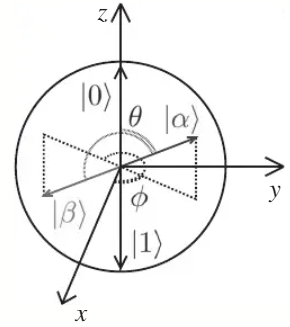
\includegraphics[width=0.3\linewidth]{Immagini - Capitolo 2/Bloch sphere.png}
        \caption{Bloch sphere.}
        \label{fig: Bloch sphere}
    \end{figure}
    Parametrising the states in terms that opposite points on the Bloch sphere correspond to orthogonal states. In general, given a generic qubit state $\ket{\alpha}$, described by parameters $\theta$ and $\phi$, the antipodal point of the corresponding Bloch vector corresponds to angles $(\pi - \theta)$ and $(\phi + \pi)$, respectively, and is associated with the qubit 
    \begin{equation}
        \begin{split}
            \ket{\beta} &= \cos{\bigg(\frac{\pi - \theta}{2}\bigg)}\ket{0} + e^{i(\phi + \pi)}\cos{\bigg(\frac{\pi - \theta}{2}\bigg)}\ket{1} \\
            &= \sin{\bigg(\frac{\theta}{2}\bigg)}\ket{0} - e^{i\phi}\cos{\bigg(\frac{\theta}{2}\bigg)}\ket{1},
        \end{split}
    \end{equation}
    and it is then straightforward to show that 
    \begin{equation}
        \begin{split}
            \mybraket{\beta}{\alpha} &= \bigg[\sin{\bigg(\frac{\theta}{2}\bigg)}\bra{0} - e^{-i\phi}\cos{\bigg(\frac{\theta}{2}\bigg)}\bra{1}\bigg]\bigg[\cos{\bigg(\frac{\theta}{2}\bigg)}\ket{0} + e^{i\phi}\sin{\bigg(\frac{\theta}{2}\bigg)}\ket{1}\bigg] \\
            &= 0.
        \end{split}
    \end{equation}
    Thus, moving from one orthonormal basis to another orthonormal one corresponds to a rotation on the Bloch sphere.
\end{ex}
The expression 
\begin{equation}
    f(\vv) = \sum_{i,j = 1}^n f_i\ve_i^*(v_j\ve_j) = \sum_{i,j = 1}^n f_iv_j\ve_i^*(\ve_j) = \sum_{i=1}^n f_iv_i
\end{equation}
can be interpreted as an inner product defined as
\begin{equation}
\label{eq: inner product}
    \inner{\cdot}{\cdot} : V^* \times V \to \C,\quad (f,\vv) \mapsto \inner{f}{\vv} = f(\vv) = \sum_{i=1}^n f_iv_i.
\end{equation}
It is important to note that the inner product defined in equation \eqref{eq: inner product} is formally different from the scalar product $\mybraket{\cdot}{\cdot} : V \times V \to \C$. Whereas the scalar product receives as its arguments an ordered pair of vectors $(\vv,\vw)$, the arguments of the inner product are a dual vector $f$ and vector $\vv$. 

Consider now two vector spaces $V$ and $W$, and the linear map $f : V \to W$; furthermore, let $g$ be a linear function $g : W \to \C$, namely $g \in W^*$. Then, also the composition map $g \circ f : V \to \C$ is linear, namely $g \circ f \in V^*$. This can be rephrased by saying that the linear map $f : V \to W$ induces a map $f^*$ from the dual vector spaces of $W$ and $V$ that is defined as
\begin{equation}
    f^* : W^* \to V^*,\quad g \mapsto g \circ f,
\end{equation}
where $f^*$ is called the pull-back of $g$. Note that for every $\vv \in V$, one can use the inner product defined in equation \eqref{eq: inner product} to define a linear function such as
\begin{equation}
    \omega_{\vv} : V^* \to \C,\quad f \mapsto \omega_{\vv}(f) = \inner{f}{\vv}.
\end{equation}
The bilinearity of the inner product implies that $\omega_{\vv}$ is an element of $V^{**}$, the dual of the dual of the vector space $V$. In fact, it is instructive to prove that every element of $V^{**}$, namely every linear function from $V^*$ to $\C$ can be constructed in this way, meaning associated with a vector $\vv \in V$. Thus, $V^{**}$ can be identified with the vector space $V$ itself, so $V^{**} \equiv V$. One can then define an action of a vector $\vv$ on a dual vector $f$ by
\begin{equation}
    \vv : V \to \C,\quad f \mapsto \vv(f) = \inner{f}{\vv} = f(\vv).
\end{equation}
Given a complex vector space $V$, one can generalise the notion of vector and dual vector and introduce a tensor of type $(p,q)$, also called a $(p,q)$-tensor defined as the following. 
\begin{defn}[$(p,q)$-tensor]
    Given a complex vector space $V$, a tensor $T$ of type $(p,q)$ is defined as a function of $p$ dual vectors and $q$ vectors that is multilinear, namely that is linear in each of its arguments, such that 
    \begin{equation}
        T : V^* \times \underbrace{\cdots}_{p\,\mathrm{times}} \times V^* \times V \times \underbrace{\cdots}_{q\,\mathrm{times}} \times V \to \C.
    \end{equation}
\end{defn}
Every linear combination $aT + bU$ of $(p,q)$-tensors $T$ and $U$ is also a $(p,q)$-tensor, hence tensors of type $(p,q)$ form a vector space; this follows from the fact that linear combinations preserve the multilinearity of the $(p,q)$-tensor. In general, the components of a $(p,q)$-tensor are defined as
\begin{equation}
    T^{i_1\cdots i_p}_{j_1\cdots j_q} = T(\ve_{i_1}^*,\dots,\ve_{i_p}^*,\ve_{j_1},\dots,\ve_{j_q}),
\end{equation}
and have $p$ upper indices and $q$ lower indices. Note also that the components of a tensor form a multidimensional array, generalising the two-dimensional array of a matrix. Tensors with more indices can be constructed from tensors with fewer indices through the tensor product operation defined as the following.
\begin{defn}[tensor product]
    Let $R$ be a tensor of type $(p,q)$ and let $S$ be a tensor of type $(l,m)$. Their tensor product $T = R \ot S$ is defined as the tensor of type $(p + l, q + m)$ such that 
    \begin{multline}
    \label{eq: tensor product of tensors}
        T(f_1,\dots,f_p,f_{p + 1},\dots,f_{p + l},\vv_1,\dots,\vv_q,\vv_{q + 1},\dots,\vv_{q+m}) = \\
        =R(f_1,\dots,f_p,\vv_1,\dots,\vv_q)S(f_{p + 1},\dots,f_{p + l},\vv_{q + 1},\dots,\vv_{q+m}).
    \end{multline}
\end{defn}
Note that the tensor product is a bilinear operation 
\begin{multline}
    (a_1R_1 + a_2R_2) \ot (b_1S_1 + b_2S_2) = \\
    = a_1b_1(R_1 \ot S_1) + a_1b_2(R_1 \ot S_2) + a_2b_1(R_2 \ot S_1) + a_2b_2(R_2 \ot S_2),
\end{multline}
for all coefficients $a_1,a_2,b_1,b_2 \in \C$. In terms of components the tensor product can be written as
\begin{equation}
\label{eq: tensor product of tensors in terms of components}
    T^{i_1\cdots i_pi_{p + 1}\cdots i_{p + l}}_{j_1\cdots j_qj_{q+1}\cdots j_{q+m}} = R^{i_1\cdots i_p}_{j_1\cdots j_q}S^{i_{p + 1}\cdots i_{p + l}}_{j_{q + 1}\cdots j_{q + m}}.
\end{equation}
One can perform repeated tensor products; the tensor product is associative 
\begin{equation}
    R \ot S \ot T = (R \ot S) \ot T = R \ot (S \ot T).
\end{equation}
Finally, one can define the operation of contraction of a tensor. This is an operation that, when applied to a $(p,q)$-tensor $T$ produces a tensor of type $(p - 1,q - 1)$denoted as $T_{c(ij)}$ and defined as
\begin{multline}
    T_{c(ij)}(f_1,\dots,f_{p - 1},\vv_1,\dots,\vv_{q - 1}) = \\ 
    = \nsum_{k}T(f_1,\dots,\underbrace{\ve_k^*}_{i\mathrm{th}},\dots,f_{p - 1},\vv_1,\dots,\underbrace{\ve_k}_{j\mathrm{th}},\dots,\vv_{q - 1}).
\end{multline}
Note that the sum over $k$ on the right-hand side of the previous expression can be rewritten in component form as 
\begin{equation}
    T_{c(ij)\,m_1\cdots m_{q - 1}}^{l_1\cdots l_{p - 1}} = \nsum_k T^{l_1\cdots l_{i - 1}l_kl_i\cdots l_{p - 1}}_{m_1\cdots m_{j - 1}m_km_j\cdots m_{q - 1}}.
\end{equation}
Thus, in contraction one chooses the $i$th upper index and the $j$th lower index to be the same label $k$, which is then summed over. 

\subsection{Tensor product of vector spaces}
As stated above, $(p,q)$-tensors form a vector space. One can arrive at this conclusion from another point of view.
\begin{defn}[tensor product of vector spaces]
    Let $V$ and $W$ be vector spaces, with $\dim{V} = n$ and $\dim{W} = m$, denoted as $V \ot W$, is the set of all finite linear combinations of tensor products $\vv \ot \vw$ with $\vv \in V$ and $\vw \in W$. If $\{\ve_i\}$ is a basis of $V$ and $\{\vf_j\}$ is a basis of $W$, then 
    \begin{equation}
        V \ot W = \sum_{i=1}^n\sum_{j=1}^m\lambda^{ij}(\ve_i \ot \vf_j),\quad \lambda^{ij} \in \C.
    \end{equation}
\end{defn}
From the tensor product definition one can see that
\begin{equation}
    \dim{(V \ot W)} = nm.
\end{equation}
An element of $V \ot W$ that can be written as $\vv \ot \vw$ for some $\vv \in V$ and $\vw \in W$ is called a ``pure tensor'' or a ``simple tensor''. Note that not all elements of $V \ot W$ are simple.
\begin{ex}
    The state 
    \begin{equation}
        \ket{\psi} = \frac{1}{\sqrt{2}}\ket{0}\ket{0} + \frac{1}{\sqrt{2}}\ket{1}\ket{1}
    \end{equation}
    is not a pure tensor, since it cannot be written as a tensor product 
    \begin{equation}
        (a\ket{0} + b\ket{1})(c\ket{0} + d\ket{1})
    \end{equation}
    for any choice of complex coefficients $a$, $b$, $c$ and $d$. Indeed this tensor product can be rewritten as
    \begin{equation}
        ac\ket{0}\ket{0} + ad\ket{0}\ket{1} + bc\ket{1}\ket{0} + bd\ket{1}\ket{1}
    \end{equation}
    and, if this expression were equal to the state $\ket{\psi}$, then the following conditions should hold
    \begin{equation}
        \begin{cases}
            ac = bd = \dfrac{1}{\sqrt{2}} \\[1.5ex]
            ad = bc = 0 \\
        \end{cases}.
    \end{equation}
    It is easy to see that there exists no solution to this system of equations: the first equation implies that neither $a$ nor $c$ can be zero; since $a$ is different from zero, $ad = 0$ implies that $d = 0$, but then $bd = 1/\sqrt{2}$ does not have any solution. 
\end{ex}
Note that, in general, $V \ot W \neq W \ot V$. However, they are isomorphism vector spaces. This follows from both having the same dimension, or by constructing an explicit isomorphic. In a similar fashion, one can construct the tensor products of dual vector spaces $V^* \ot W^*$ and of a vector space and a dual vector space $V \ot W^*$. This is easiest using a basis and a dual basis
\begin{align}
    V^* \ot W^* &= \sum_{i=1}^n\sum_{j=1}^m\lambda_{ij}(\ve^{*i} \ot \vf^{*j}),\quad \lambda_{ij} \in \C, \\
    V \ot W^* &= \sum_{i=1}^n\sum_{j=1}^m\lambda_j^i(\ve_i \ot \vf^{*j}),\quad \lambda_i^j \in \C.
\end{align}
Note that elements $L = \sum_{i=1}^n\sum_{j=1}^m\lambda_j^i(\ve_i \ot \vf^{*j})$ of $V \ot W^*$ are linear operators $L : W \to V$. This can be seen by denoting 
\begin{equation}
    L = \sum_{i=1}^n\sum_{j=1}^m\lambda_j^i\ket{i}\bra{j}
\end{equation}
and by expanding a vector $\ket{\chi} \in W$ in the basis $\ket{j}$ such that $\ket{\chi} = \sum_{k=1}^m\chi_k\ket{k}$, then $L$ acts on it by 
\begin{equation}
    L\ket{\chi} = \sum_{i=1}^n\sum_{j=1}^m\sum_{k=1}^n\lambda^i_j\chi_k\ket{i}\mybraket{j}{k} = \sum_{i=1}^n\sum_{j=1}^m\lambda^i_j\chi_j\ket{i},
\end{equation}
so $L\ket{\chi}$ is a vector in $V$ with components $\sum_{j=1}^m\lambda^i_j\chi_j$, indexed by the free index $i$. Since the tensor product space is a vector space, one can perform a tensor product of that with another vector space. The tensor product is associative, in the sense that is a natural isomorphism $(V_1 \ot V_2) \ot V_3 \simeq V_1 \ot (V_2 \ot V_3)$, so that one can write $V_1 \ot V_2 \ot V_3$ for short. Now, $(p,q)$-tensors can be defined in an alternative way by first defining a vector space
\begin{equation}
    T^p_q(V) = V \ot \underbrace{\cdots}_{p\,\mathrm{times}} \ot V \ot V^* \ot \underbrace{\cdots}_{q\,\mathrm{times}} \ot V^*.
\end{equation}
Using the basis, elements $T \in T^p_q(V)$ can be expanded as
\begin{equation}
    T = \sum_{\substack{i_1,\dots,i_p \\ j_1,\dots,j_q}}T^{i_1\cdots i_p}_{j_1\cdots j_q}(\ve_{j_1} \ot \cdots \ot \ve_{i_p} \ot \ve_{*j_1} \ot \cdots \ot \ve_{*j_q}).
\end{equation}
Hence, the elements $T \in T^p_q(V)$ can be recognised as $(p,q)$-tensors; this can be taken as their alternative definition. Acting with $T$ on the basis vectors projects out its components $T^{i_1\cdots i_p}_{j_1\cdots j_q}$. 
\begin{notz}
    At this point the Einstein summation convention will be used: repeated indices are understood to be summed over, and the explicit summation symbols $\Sigma$ are not shown. Thus, for example one has
    \begin{equation}
        T = T^{i_1\cdots i_p}_{j_1\cdots j_q}(\ve_{j_1} \ot \cdots \ot \ve_{i_p} \ot \ve^{*j_1} \ot \cdots \ot \ve^{*j_q}).
    \end{equation}
\end{notz}
The tensor components satisfy a characteristic transformation rule under a change of basis. For notational brevity, consider only a $(1,2)$-tensor. Let $\ve_k' = R_k^l\ve_l$ and $\vf^{*i} = S^i_j\ve^{*j}$ be the transformation between two orthonormal bases $\{\ve_i\}$ and $\{\ve_i'\}$. Since $\vf^{*i}(\vf_k) = \ve^{*i}(\ve_k) = \delta^i_k$, one must have
\begin{equation}
    \delta^i_k = \vf^{*i}(\ve_k') = S^i_jR^l_ke^{*j}(\ve_l) = S^i_jR^l_K\delta^j_l = S^i_jR^j_k,
\end{equation}
which means that $S$ is the inverse of $R$, namely $S^i_j = (R^{-1})^i_j$. Denoting the components of a $(1,2)$-tensor in the two bases as $T^i_{jk}$ and $T'^{i}_{jk}$, one gets
\begin{equation}
    \begin{split}
        T &= T'^i_{jk}(\vf_i \ot \vf^{*j} \ot \vf^{*k}) \\
        &= T'^i_{jk}R^l_i(R^{-1})^j_m(R^{-1})^k_n(\ve_l \ot \ve^{*m} \ot \ve^{*n}) \\
        &= T^l_{mn}(\ve_l \ot \ve^{*m} \ot \ve^{*n}),
    \end{split}
\end{equation}
so that the components transform as
\begin{equation}
    T^l_{mn} = R^l_i(R^{-1})^j_m(R^{-1})^k_nT'^i_{jk}.
\end{equation}
Transformation rules for other $(p,q)$-tensors can be derived in a similar manner. 
\begin{notz}
    It is convenient to introduce a tensor power notation; given a non-negative integer $n$, one can write
    \begin{equation}
        V^{\ot n} = V \ot \underbrace{\cdots}_{n\,\mathrm{times}} \ot V,
    \end{equation}
    which can be used to write $T^p_q(V) = V^{\ot p} \ot V^{*\ot q}$.
\end{notz}
Let's now consider the tensor product defined in equation \eqref{eq: tensor product of tensors}. It should correspond to the product map $T^p_q(V) \ot T^m_n(V) \to T^{p + m}_{q + n}(v)$. There is one subtlety in making contact with equation \eqref{eq: tensor product of tensors}. Consider, for example, the tensor product of a $(1,1)$-tensor $R$ with a $(1,0)$-tensor $S$. At first one can attempt 
\begin{equation}
    R \ot S = (R^i_j\ve_i \ot \ve^{*j}) \ot (S^k\ve_k) = R^i_jS^k\ve_i \ot \ve^{*j} \ot \ve_k.
\end{equation}
However, the expansion of a $(2,1)$-tensor involves the basis vectors $\ve_i \ot \ve_j \ot \ve^{*k}$ rather than $\ve_i \ot \ve^{*j} \ot \ve_k$, and the tensor product is not commutative. One has to define the tensor product $R \ot S$ in such a way that all basis vectors of $V$ and dual basis vectors of $V^*$ are grouped together. That is, instead what first attempted one defines
\begin{equation}
    R \ot S = R^i_kS^j(\ve_i \ot \ve_j \ot \ve^{*k}).
\end{equation}
Now, consider again a $(p,q)$-tensor $R$ and a $(m,n)$-tensor $S$. Expanding both
\begin{align}
    R &= R^{i_1\cdots i_p}_{j_1\cdots j_q}(\ve_{i_1} \ot \cdots \ot \ve_{i_p} \ot \ve^{*j_1} \ot \cdots \ot \ve^{*j_q}), \\
    S &= S^{k_1\cdots k_p}_{l_1\cdots l_q}(\ve_{k_1} \ot \cdots \ot \ve_{k_p} \ot \ve^{*l_1} \ot \cdots \ot \ve^{*l_q}),
\end{align}
the tensor product $T = R \ot S$ can be built as
\begin{equation}
    \begin{split}
        T &= R^{i_1\cdots i_p}_{j_1\cdots j_q}S^{k_1\cdots k_m}_{l_1\cdots l_n}(\ve_{i_1} \ot \cdots \ot \ve_{i_p} \ot \ve_{k_1} \ot \cdots \ot \ve_{k_m} \\
        &\ot \ve^{*j_1} \ot \cdots \ot \ve^{*j_q} \ot \ve^{*l_1} \ot \cdots \ve^{*l_n}) \\
        &= R^{i_1\cdots i_p}_{j_1\cdots j_q}S^{i_{p + 1}\cdots i_{p + m}}_{j_{q + 1}\cdots j_{q + n}}(\ve_{i_1} \ot \cdots \ot \ve_{i_p} \ot \ve_{i_{p + 1}} \ot \cdots \ot \ve_{i_{p + m}} \\
        &\ot \ve^{*j_1} \ot \cdots \ot \ve^{*j_q} \ot \ve^{*j_{q + 1}} \ot \cdots \ve^{*j_{q + m}}),
    \end{split}
\end{equation}
in agreement with equation \eqref{eq: tensor product of tensors in terms of components}.

\subsection{Tensor product of linear operators}
Since elements $L \in W \ot V^*$ are linear operators $L : V \to W$, conversely one can represent every linear operator from $V$ to $W$ in a tensor product basis. Let $\{\ve_i\}$ be an orthonormal basis in $V$ and let $\{\vf_k\}$ be an orthonormal basis of $W$. Every linear operator $A : V \to W$ is then uniquely determined by its components with respect to the two bases. One can then identify the linear operator with the matrix having these components as its entries, $A = (A)^i_j$. One way to explicitly extract the components is to use the scalar product in $W$ and let $A$ act on the basis vector of $V$ by
\begin{equation}
    A^i_j = \mybraket{\vf_i}{A\ve_j}.
\end{equation}
Another way to extract the components of $A$ is to use the dual basis $\{\vf^{*i}\}$ of $W^*$ and compute the inner products
\begin{equation}
    A^i_j = \mybraket{\vf^{*i}}{A\ve_j}.
\end{equation}
When acting on a vector $\vv = v^k\ve_k \in V$, it gives
\begin{equation}
    A\vv = A^i_J\vf_i\ve^{*j}(v^k\ve_k) = A^i_jv^k\vf_i\ve^{*j}(\ve_k) = A^i_jv^k\delta^j_k\vf_i = A^i_j\ve^j\vf_i,
\end{equation}
which is a vector of $W$ with components $A^i_jv^j$, as expected. Note the product of the matrix $(A)^i_j$ and the vector $\vv^j$. In quantum mechanics it is often very useful to construct tensor products of linear operators. 
\begin{defn}[tensor product of linear operators]
    Let $A : V_1 \to V_2$ and $W : W_1 \to W_2$ be two linear operators. The tensor product of linear operators is defined by first imposing the action on the simple tensor of $V_1 \ot W_1$ as
    \begin{equation}
        (A \ot B)(\vv \ot \vw) = A(\vv) \ot B(\vw),\quad \forall \vv \ot \vw \in V_1 \ot W_1;
    \end{equation}
    next, choosing a basis $\basis_{V_1} = \{\ve_i\}$ and $\basis_{W_1} = \{\vf_j\}$, by imposing the action of $(A \ot B)$ on a generic $(2,0)$-tensor $T = T^{ij}(\ve_i \ot \vf_j)$ in $V_1 \ot W_1$ as
    \begin{equation}
        A \ot B : V_1 \ot W_1 \to V_2 \ot W_2,\quad T \mapsto (A \ot B)(T) = T^{ij}A(\ve_i) \ot B(\vf_j);
    \end{equation}
    thus, expanding the linear operators in a basis, the expansion of their tensor product becomes
    \begin{equation}
        A \ot B = A^i_jB^k_l(\ve_i \ot \ve_k \ot \vf^{*j} \ot \vf^{*l})
    \end{equation}
\end{defn}
As before, the next step is to generalise this definition to multiple tensor products of linear operators. Let $T \in V_1 \ot \cdots \ot V_n$, then 
\begin{equation}
    (A_1 \ot \cdots \ot A_n)(T) = T^{i_1\cdots i_n}A_1(\ve_{i_1}) \ot \cdots \ot A_n(\ve_{i_n}),
\end{equation}
where $A_k$ are linear operators $A_k : V_k \to W_k$. Generalising further, one can then form linear combinations of tensor products of linear operators, to construct more general linear operators acting on $V_1 \ot \cdots \ot V_n$. Let $\{A_k^{(r)}\}$, with $r = 1,\dots,s$, be a collection of linear operators from $V_k$ to $W_k$, then the operator $A$ is defined a 
\begin{equation}
    A = \sum_{r=1}^sc_r(A_1^{(r)} \ot \cdots \ot A_n^{(r)}),\quad c_r \in \C,
\end{equation}
is a linear operator $A : V_1 \ot \cdots \ot V_n \to W_1 \ot \cdots \ot W_n$. For this type of generic operator $A$ acting on a tensor product of vectors spaces, there is no reason to try to break up its components into a sum of products; instead, one can use the generic tensor component notation and write
\begin{equation}
    A = A^{i_1\cdots i_n}_{j_1\cdots j_n}\ket{i_1,\dots,i_n}\bra{j_1,\dots,j_n}.
\end{equation}
The tensor product is closely related to the Kronecker product of matrices, defined as the following.
\begin{defn}[Kronecker product]
    Let $A$ be an $N \times N$ matrix with components $a_{ij}$ and let $B$ be an $M \times M$ matrix with components $b_{ij}$. The Kronecker product $A \ot B$ of the matrices is defined to be an $NM \times NM$ matrix with the structure
    \begin{equation}
        \begin{split}
            A \ot B &= 
            \begin{pmatrix}
                a_{11} & \cdots & a_{1N} \\
                \vdots & \ddots & \vdots \\
                a_{N1} & \cdots & a_{NN}
            \end{pmatrix} \ot
            \begin{pmatrix}
                b_{11} & \cdots & b_{1M} \\
                \vdots & \ddots & \vdots \\
                b_{M1} & \cdots & b_{MM}
            \end{pmatrix} \\
            &= 
            \begin{pmatrix}
                a_{11}B & \cdots & a_{1N}B \\
                \vdots & \ddots & \vdots \\
                a_{N1}B & \cdots & a_{NN}B
            \end{pmatrix} \\
            &= 
            \begin{pmatrix}
                a_{11}b_{11} & \cdots & a_{11}b_{1M} & a_{12}b_{11} & \cdots & a_{1N}b_{1M} \\
                \vdots & \ddots & \vdots & \vdots & \ddots & \vdots \\
                a_{N1}b_{M1} & \cdots & a_{N1}b_{MM} & a_{N2}b_{M1} & \cdots & a_{NN}b_{MM}
            \end{pmatrix}.
        \end{split}
    \end{equation}
\end{defn}
The Kronecker product of two matrices in not commutative, namely $A \ot B \neq B \ot A$, but the two resulting matrices can be mapped into each other by a permutation of rows and columns. Furthermore, the Kronecker $\vv \ot f$ between a vector and a dual vector yields an $N \times N$ matrix
\begin{equation}
    \vv \to f =
    \begin{pmatrix}
        v^1 \\
        \vdots \\
        v^N
    \end{pmatrix} \ot
    \begin{pmatrix}
        f_1,\dots,f_N
    \end{pmatrix} = 
    \begin{pmatrix}
        v^1f_1 & \cdots & v^1 \\
        \vdots & \ddots & \vdots \\
        v^Nf_1 & \cdots & v^Nf_N
    \end{pmatrix}.
\end{equation}
In a similar way, the Kronecker product of a vector $\vv$ with $N$ components and a vector $\vw$ with $M$ components is a vector with $NM$ components
\begin{equation}
    \vv \ot \vw = 
    \begin{pmatrix}
        v^1 \\
        \vdots \\
        v^N
    \end{pmatrix} \ot 
    \begin{pmatrix}
        w^1 \\
        \vdots \\
        w^M
    \end{pmatrix} =
    \begin{pmatrix}
        v^1\vw \\
        \vdots \\
        v^N\vw
    \end{pmatrix} = 
    \begin{pmatrix}
        v^1w^1 \\
        \vdots \\
        v^1w^M \\
        \vdots \\
        v^Nw^1 \\
        \vdots \\
        v^Nw^M
    \end{pmatrix}.
\end{equation}
Likewise, a product of a dual row vector $f$ with $N$ components and a dual row vector $g$ with $M$ components is a dual row vector with $NM$ components. Now, let $A$ be a linear operator on $V$ with $\dim{V} = N$ and $B$ a linear operation on $W$ with $\dim{W} = M$. Given a basis in $V$ and one in $W$, the operators can be identified with the matrices of their coefficients and their tensor product $A \ot B$ becomes the Kronecker product of the matrices, resulting in an $NM\times NM$ matrix. The trace of this matrix is taken over the tensor product basis $\{\ket{i},\ket{j}\}$, with $1 \le i \le N$ and $1 \le j \le M$, of $V \ot W$ as
\begin{equation}
    \begin{split}
        \tr{(A \ot B)} = \sum_{i=1}^N\sum_{j=1}^M\mybrakett{i}{\mybrakett{i}{(A \ot B)}{j}}{j} &= \sum_{i=1}^N\sum_{j=1}^M\mybrakett{i}{A}{i}\mybrakett{j}{B}{j} \\
        &= \sum_{i=1^N}\mybrakett{i}{A}{i}\sum_{j=1}^M\mybrakett{j}{B}{j},
    \end{split}
\end{equation}
from where it is immediate to see the property of the trace
\begin{equation}
    \tr{(A \ot B)} = \tr{(A)}\tr{(B)}.
\end{equation}
A similar property holds for the determinant of said matrix, in particular
\begin{equation}
    \det{(A \ot B)} = (\det{A})^M(\det{B})^N.
\end{equation}

\subsection{Heisenberg spin chain}
The quantum Heisenberg spin chain is an elementary model of magnets. A ferromagnetic material can be thought of as consisting particles with a magnetic moment. When the alignment of the elementary magnets has a preferred direction, which is observable on a macroscopic scale the material appears to be magnetic. At the microscopic level, the existence of the magnetic moments can be interpreted in terms of the spin of particles; for example, an electron acts like a tiny bar magnet with a dipole magnetic field, associated with a magnetic moment $\vmu = -g_s\mu_Bm\vs$, where $g_s$ is called the spin $g$-factor, $\mu_B$ is the Bohr magneton and $m = \pm1/2$ is the spin quantum number. Quantum Heisenberg spin chains are models of one-dimensional lattices of elementary magnetic moments, with nearest-neighbour interactions that tend to make neighbouring magnetic moments aligned an parallel, or aligned and oppositely oriented, resulting in a net magnetisation. Start by considering linear operation of the form 
\begin{equation}
\label{eq: linear operator (Heisenberg spin chain)}
    \MI_2 \ot \cdots \ot \MI_2 \ot \sigma^a_k \ot \sigma^b_{k + 1} \ot \MI_2 \cdots \ot \MI_2,
\end{equation}
where the subscripts $k$ and $k + 1$ have been to the Pauli matrices to emphasize that they act on the electrons at the $k$th site and the $(k + 1)$th site, respectively. Acting on a basis state
\begin{equation}
    \ket{i_1\cdots i_{k-1}i_ki_{k+1}\cdots i_N} = \ket{i_1} \ot \cdots \ot \ket{i_{k-1}} \ot \ket{i_k} \ot \ket{i_{k+1}} \ot \cdots \ot \ket{i_N}
\end{equation}
the operator defined in equation \eqref{eq: linear operator (Heisenberg spin chain)} produces the state
\begin{equation}
    \ket{i_1} \ot \cdots \ot \ket{i_{k-1}} \ot \sigma^a\ket{i_k} \ot \sigma^b\ket{i_{k+1}} \ot \cdots \ot \ket{i_N}.
\end{equation}
Suppressing the unit matrices in the definition of the operator introduced in equation \eqref{eq: linear operator (Heisenberg spin chain)} for a shorter notation, one can define a set of local operators, labelled by $k$, of the form
\begin{equation}
\label{eq: set of local linear operators (Heisenberg spin chain)}
    \hatH_{k,k + 1} = \frac{\lambda}{2}\bigg(\MI_k \ot \MI_{k + 1} - \sum_{a=1}^3\sigma^a_k \ot \sigma^a_{k + 1}\bigg),
\end{equation}
where $\lambda \in \R$ is a parameter controlling the strength and alignment of the nearest-neighbour interactions. Finally, by summing over the sites, one constructs the Hamiltonian operator as
\begin{equation}
    \hatH = \sum_{k=1}^{N-1}\hatH_{k,k + 1}.
\end{equation}
This is the Heisenberg XXX quantum spin chain. Note that there exist other variants of Heisenberg spin chains, with different Hamiltonian operators. Also, one can either assume the sites to be arranged in a periodic chain, identifying the first and the $N$th site, and letting the sum run up to $N$, which yields a closed spin chain, or having an infinite lattice with the sum running over all integers, which corresponds to an infinite chain. The Hamiltonian has a discrete set of degenerate eigenvalues $E_n$ and eigenstates $\ket{\psi_n}$, which satisfy 
\begin{equation}
    \hatH\ket{\psi_n} = E_n\ket{\psi_n}.
\end{equation}
When $\lambda > 0$, the interaction defined in equation \eqref{eq: set of local linear operators (Heisenberg spin chain)} tends to align the neighbouring spins: in that case, the interaction and the resulting ground state, with energy $E_0$, are said to be ferromagnetic; conversely, for $\lambda < 0$, the interaction and the ground state are called anti-ferromagnetic. The model has a $SU(2)$ symmetry which helps in finding and organising the eigenstates. Defining
\begin{equation}
    J^a = \frac{1}{2}\sum_{k=1}^N\sigma^a_k,
\end{equation}
it is easy to see that $J^a$ operators satisfy the commutation relations of the generators of the $SU(2)$ Lie group $\comm{J^a}{J^b} = i\epsilon^{abc}J^c$. Moreover, one can show that they commute with the Hamiltonian, $\comm{J^a}{H} = 0$ for any $a \in \{1,2,3\}$. This means that the Heisenberg XXX spin chain has an $SU(2)$ symmetry, then the energy eigenstates for every $E_n$ correspond to irreducible spin-$j$ representations of the $SU(2)$ group. Note that the discussion started with the smallest irreducible two-dimensional representation for a single electron, but as a result of taking $N$ copies it ended with a $2^N$-dimensional vector space $V$. The action of $SU(2)$ on $V$ is reducible. Since every state can be expressed in the basis of energy eigenstates, which belong to irreducible representations, studying the energy eigenstates of this system corresponds to solving the reduction problem.

\chapter{Lie groups and Lie algebras}
In this chapter, there will be introduced some general concepts about properties of Lie algebras and groups, and their unitary representations, while on the other hand there will be a special focus on the irreducible representations of the $\sua(N)$ Lie algebras and of the corresponding $SU(N)$ Lie groups. This is motivated in part by particle physics, since the Standard Model is based on the $U(1) \times SU(2) \times SU(3)$ gauge symmetry with various proposed extension involving higher-dimensional $SU(N)$ groups. In addition, $SU(N)$ Lie groups also have important applications in condensed matter theory and other areas of physics. 

First, the definition of a Lie group is recalled, though in a more precise way.
\begin{defn}[Lie group]
    A Lie group $G$ is a differentiable manifold with a group internal operation $\cdot : G \times G \to G$, $(g,g') \mapsto g'' \in G$ for any $g,g' \in G$, such that:
    \begin{enumerate}
        \item is associative, namely $g\cdot(g'\cdot g'') = (g\cdot g')\cdot g''$, for any $g,g',g'' \in G$;
        \item there exists a unit element $e \in G$ such that $e\cdot g = g\cdot e = g$ for every $g \in G$;
        \item there exists an inverse element $g^{-1} \in G$ such that $g^{-1}\cdot g = g\cdot g^{-1} = e$ for every $g \in G$;
        \item is smooth to guarantee that the multiplication and inverse operation are also smooth, namely that requires the smoothness of the map $(g,g') \mapsto g^{-1}g'$ for any $g,g' \in G$.
    \end{enumerate}
\end{defn}
\begin{defn}[Lie subgroup]
    A subgroup $H$ of a Lie group $G$ is a Lie subgroup if the inclusion map $i : H \to G$, $i(h) = h$ is an injective immersion, namely an embedding of $H$ into $G$ as a submanifold, and a group homomorphism.
\end{defn}
Examples of Lie groups were already previously encountered, namely the matrix Lie groups $GL(n,\R)$ and $GL(n,\C)$, and their subgroups $SL(n,\R)$, $SL(n,\C)$, $O(n)$, $U(n)$, $SO(n,\R)$ and $SU(n)$. However, the focus will be narrowed to compact Lie groups, whose set contains the $U(1)$, $O(n)$, $SO(n)$, $U(n)$, $SU(n)$ and $Sp(n)$ groups, the compact forms of the exceptional Lie groups $\G_2$, $\F_4$, $\E_6$, $\E_7$ and $\E_8$, and all of their finite direct product groups. For clearness, a compact Lie group is one that is closed and limited. To define a Lie algebra it is necessary to first define what is an algebra. 
\begin{defn}[algebra]
    An algebra is a vector space $V$ over a field $K$ which also has an internal operation $\cdot : V \times V \to V$ that for every element $X,Y,Z \in V$ and $a,b,c \in K$ satisfies the following properties:
    \begin{enumerate}
        \item left distributivity, namely $(aX + bY)\cdot Z = a(X \cdot Z) + b(Y\cdot Z)$;
        \item right distributivity, namely $X \cdot (aY + bZ) = a(X\cdot Y) + b(X \cdot Z)$;
        \item compatibility with scalars, namely $(aX)\cdot(bY) = (ab)(X \cdot Y)$.
    \end{enumerate}
\end{defn}
Then, a Lie algebra is an algebra that satisfies some additional requirements.
\begin{defn}[Lie algebra]
    A Lie algebra is an algebra over a field $K$ equipped with the internal operation $\comm{\dots}{\dots} : V \times V \to V$, called the Lie bracket, which for every element $X,Y,Z \in V$ and $a,b,c \in K$ satisfies the following properties:
    \begin{enumerate}
        \item linearity in the first argument, namely $\comm{aX + bY}{Z} = a\comm{X}{Z} + b\comm{Y}{Z}$;
        \item antisymmetric, namely $\comm{X}{Y} = - \comm{Y}{X}$;
        \item it satisfies the Jacobi identity $\comm{X}{\comm{Y}{Z}} + \comm{Y}{\comm{Z}{C}} + \comm{Z}{\comm{X}{Y}} = 0$.
    \end{enumerate}
\end{defn}
Note that the first two statements of the Lie algebra definition imply linearity also in the second argument, making the Lie algebra bilinear just like the general definition of an algebra require.
\begin{defn}[Abelian Lie algebra]
    A Lie algebra is said to be Abelian if the Lie bracket is commutative, namely if $\comm{X}{Y} = 0$ for any $X,Y \in V$.
\end{defn}
There are other useful definitions that regard subspaces of the vector space $V$.
\begin{defn}[Lie subalgebra]
    If a subspace $W \subset V$ is closed under the Lie bracket, namely if $\comm{X}{Y} \in W$ for any $X,Y \in W$, it is a Lie subalgebra of $V$.
\end{defn}
\begin{defn}[ideal]
    If $\comm{X}{Y} \in W$ for every element $X \in W \subseteq V$ and every element $Y \in V$, then $W \subseteq V$ is called an ideal, or an invariant Lie subalgebra.
\end{defn}
Note that $W = V$ and $W = \{\vo\}$ are always ideals, for this they are called trivial ideals. Conversely, a non-trivial ideal is an ideal that is a proper subset of $V$. The possible existence of non-trivial ideals leads to the introduction of the two following definitions.
\begin{defn}[simple Lie algebra]
    A Lie algebra is said to be simple if it has no non-trivial ideals.
\end{defn}
\begin{defn}[semi-simple Lie algebra]
    A Lie algebra is said to be semi-simple if it has no non-trivial Abelian ideals.
\end{defn}
From these definitions, it follows that all simple Lie algebras are also semi-simple, while the converse statement is not true. In general, semi-simple algebras are direct sums of simple ones. 

To define a Lie algebra, a vector space is first needed. Since a Lie group $G$ is a smooth manifold, one can use the space of vector fields on $G$. However, it will be added one powerful requirement and restrict to a specific set of vector fields. Consider now a manifold $M$ and curve $\curve$ on said manifold, defined as $\curve(t) : (a,b) \to M$ with $t \in (a,b) \subseteq \R$ where it assumed that $0 \in (a,b)$. 
\begin{figure}[h]
    \centering
    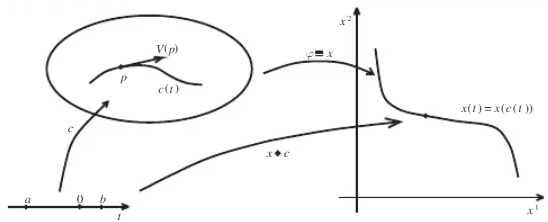
\includegraphics[width=0.7\linewidth]{Immagini - Capitolo 3/curve on manifold.png}
    \caption{a curve $\curve(t)$ on and a tangent vector $v_P$ at $P = \curve(0)$.}
    \label{fig: curve on manifold}
\end{figure}
Let $P \in M$ be a point on the manifold set to be $P \equiv \curve(0)$, and define the vector $v_P$ that is tangent to the curve $\curve$ in the point $P$, namely the tangent vector in a point $P$ of a manifold $M$, as
\begin{equation}
\label{eq: tangent vector on a manifold}
    v_P := v^\mu(P)\frac{\p}{\p x^\mu} = \frac{d}{dt}x^\mu[\curve(t)]\bigg|_{t = 0}\frac{\p}{\p x^\mu}.
\end{equation}
If one defines the function $f : M \to \R$, then, with the previous definition in \eqref{eq: tangent vector on a manifold}, the change in $f$ along the curve $\curve$ can be expressed as
\begin{equation}
    \frac{df}{dt} \equiv v_P[f] = \frac{d}{dt}x^\mu[\curve(t)]\bigg|_{t = 0}\frac{\p f}{\p x^\mu},
\end{equation}
which is precisely the total derivative of $f$ computed along the curve $\curve$. From the definition in \eqref{eq: tangent vector on a manifold}, it follows the next definition.
\begin{defn}[tangent vector space]
    The tangent vectors space $T_PM$ is defined as the set of all tangent vectors $v_P$, and all the possible linear combinations, in a point $P$ of a manifold $M$.
\end{defn}
Since the notion of a dual vector space is understood, it is possible to give the following definition.
\begin{defn}[dual tangent vectors space]
    The dual tangent vectors space $T^*_PM$, also called the cotangent vector space, is the dual vector space of $T_PM$ and it is defined as the set of all linear functions from $T_PM$ to $\R$.
\end{defn}
Consider now two manifolds $M$ and $N$, define a function $f : M \to N$ and let $P$ be a point on $M$, with image $f(P)$ as a point on $N$, as shown in figure \ref{fig: pushforward}, one can define the vector spaces $T_PM$ and $T_{f(P)}M$. Furthermore, given a function $g : N \to \R$, one can construct the composite function $g \circ f : M \to \R$ and ask how this function changes along a curve having $v$ as the tangent vector in $P \in M$. The answer is given by defining the push-forward of $f$ of said tangent vector as 
\begin{equation}
    (f_*v)[g] = v[g \circ f].
\end{equation}
In other words, if $v$ is a tangent vector of a curve $\curve(t)$, so that $v[g \circ f]$ characterises the rate of change of a function $g \circ f$ along the curve $\curve(t)$, then $f_*v$ characterises the rate of change of the function $g$ along the image curve $f(\curve(t))$. The components of the push-forward are
\begin{equation}
    (f_*v)^\nu = v^\mu\frac{\p y(x^\nu)}{\p x^\mu},\quad y^\mu(x^\nu) \equiv f(x^\nu(\curve(t))).
\end{equation}
\begin{figure}[h]
    \centering
    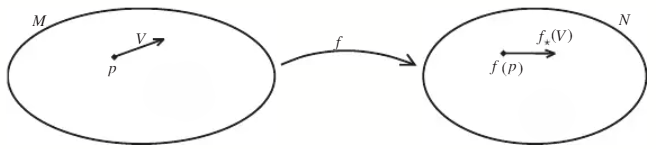
\includegraphics[width=0.7\linewidth]{Immagini - Capitolo 3/pushforward.png}
    \caption{push-forward $f_*v$ of a tangent vector $v \in T_PM$.}
    \label{fig: pushforward}
\end{figure}

Given an element $a \in G$ of a Lie group $G$, one can define the left action as the left translation $L_a : G \to G$, $g \mapsto L_a(g) = a\cdot g$, which is a diffeomorphism\footnote{Since the product must be a smooth map and one of its elements is fixed.}. Then one is going to use the associated push-forward $(L_a)_*$, which maps a tangent vector at $g$ to a tangent vector at $a \cdot g$. In general, given a vector field $X$ on $G$, one could look at its values at points $g$ and $a \cdot g$ to obtain two tangent vectors, however in general these two have no simple relation. Requiring that $X|_g$ is related to $X|_{a\cdot g}$ by the push-forward map, the following definition can be stated.
\begin{defn}[invariant vector field]
    A vector field $X$ on a group $G$ is left-invariant if $(L_a)_* : T_gG \to T_{a\cdot g}G$ satisfies the following condition 
    \begin{equation}
        (L_a)_*X|_g = X|_{a\cdot g}.
    \end{equation}
\end{defn}
This definition can be extended to Lie algebras.
\begin{defn}[invariant Lie algebra]
    A Lie algebra is defined as the set of left-invariant vector fields $\algebra$ on the group $G$ with the commutator defined as 
    \begin{equation}
        \comm{X}{Y} := XY - YX,
    \end{equation}
    where $X$ and $Y$ are vector fields on $G$.
\end{defn}
The set $\algebra$ is a vector space, since the push-forward $(L_g)_*$ is a linear map, and is isomorphic to $T_eG$, hence its dimension is $\dim{\algebra} = \dim{G}$. Since $\algebra$ is also a collector of fields, their commutators can be computed; the result is again left-invariant
\begin{equation}
    (L_a)_*\comm{X}{Y}|_g = \comm{(L_a)_*X|g}{(L_a)_*Y|_g}.
\end{equation}
In turn, using left-invariance, one has $\comm{(L_a)_*X|g}{(L_a)_*Y|_g} = \comm{X|_{a\cdot g}}{Y|_{a\cdot g}}$, hence 
\begin{equation}
    (L_a)_*\comm{X}{Y}|_g = \comm{X|_{a\cdot g}}{Y|_{a\cdot g}} \equiv \comm{X}{Y}|_{a\cdot g}.
\end{equation}
Thus, if $X$ and $Y$ are two arbitrary elements of $\algebra$, then also $\comm{X}{Y}$ is an element of $\algebra$. It is now justified to define a Lie algebra in the following way.
\begin{defn}[Lie algebra]
    A Lie algebra of a Lie group $G$ is the set of left-invariant vector fields $\algebra$ with the commutator $\comm{\dots}{\dots} : \algebra \times \algebra \to \algebra$, $(X,Y) \mapsto \comm{X}{Y}$.
\end{defn}
Note that since $\algebra$ is isomorphic to the tangent space of the Lie group at the identity $T_eG$, it is also justified to consider the latter as the Lie algebra associated with the Lie group. Recall also that in equation \eqref{eq: tangent vector on a manifold} the tangent vector $v$ was defined as an operator associated with a curve $\curve(t)$, or an equivalence class of curves giving the same tangent vector, at a point $P \equiv \curve(0)$, and there was a one-to-one correspondence between equivalence classes of curves and tangent vectors. This definition is useful to find the Lie algebras associated with some matrix Lie groups. For this purpose, it is useful to introduce the following identity 
\begin{equation}
\label{eq: positive matrix identity}
    \det{M} = \exp{(\tr{\ln{M}})},
\end{equation}
for a positive definite matrix $M$, so 
\begin{equation}
    \begin{split}
        \det{(\MI_n + A)} = \exp{[\tr{\ln{(\MI_n + A)}}]} &\simeq \exp{\bigg[\tr{\bigg(A - \frac{A^2}{2} + \cdots \bigg)}\bigg]} \\
        &\simeq 1 + \tr{A} + \cdots.
    \end{split}
\end{equation}
\begin{ex}
    If the Lie algebra is identified with the tangent space at unity, one can construct the Lie algebras of common matrix groups:
    \begin{enumerate}
        \item for $\gla(n,\R)$, it is immediate to get $\gla(n,\R) = \{A \in \R^{n,n}\} \equiv \R^{n,n}$;
        \item for $\sla(n,\R)$, consider a curve $\curve(t)$ that passes through the unit element $e = \MI_n \in SL(n,\R)$ with $e \equiv \curve(0)$ and derive the tangent vector at $t = 0$, thus for small $t$ the curve can be approximated as $\curve(t) \simeq \MI_n + tA + \cdots$, so the tangent vector is found to be
        \begin{equation}
            \frac{d\curve(t)}{dt}\bigg|_{t = 0} = A \in T_eSL(n,\R),
        \end{equation}
        so now by using the relation \eqref{eq: positive matrix identity} and the unit determinant condition one can write
        \begin{equation}
            1 = \det{\curve(t)} = \det{(\MI_n + A)} \simeq 1 + t\tr{A} + \cdots,
        \end{equation}
        thus resulting in $\tr{A} = 0$ and identifying 
        \begin{equation}
            \sla(n,\R) = \{A \in \R^{n,n} : \tr{A} = 0\};
        \end{equation}
        \item for $\soa(n)$, consider a curve $\curve(t) = \MI_n + tA$ and require it to be orthogonal 
        \begin{equation}
            \MI_n = \curve(t)\curve(t)^T = (\MI_n + tA)(\MI_n + tA)^T = \MI + t(A + A^T) + o(t^2),
        \end{equation}
        thus resulting in $A = -A^T$, so one can identify the $\soa(n)$ algebra as the set of antisymmetric real matrices
        \begin{equation}
            \soa(n) = \{A \in \R^{n,n} : A = -A^T\};
        \end{equation}
        \item for $\ua(n)$, consider the curve $\curve(t) = \MI_n + tA$ and impose the unitarity condition
        \begin{equation}
            \MI_n = \curve(t)\curve(t)^\dg = (\MI_n + tA)(\MI_n + tA)^\dg = \MI + t(A + A^\dg) + o(t^2),
        \end{equation}
        to find the constraint $A = -A^\dg$, hence $\ua(n)$ can be identified with the set of anti-Hermitian complex matrices; however in Physics, since in quantum mechanics the observable correspond to Hermitian operators, is more frequent to use the convention in which $t$ is multiplied by the imaginary unit, so by using the curve $\curve(t) = \MI_n + itA$ that leads to the constraint $A = A^\dg$, resulting in the identification
        \begin{equation}
            \ua(n) = \{A \in \C^{n,n} : A = A^\dg\};
        \end{equation}
        \item for $\sua(n)$, imposing the unitarity and the unit determinant conditions, using physics conventions, results in the identification
        \begin{equation}
            \sua(n) = \{A \in \C^{n,n} : A = A^\dg,\,\tr{A} = 0\}.
        \end{equation}
    \end{enumerate}
\end{ex}
Conversely, one can construct elements of the group from elements of the associated algebra using the exponential map, defined as the mapping from a Lie algebra $\algebra$ to the associated Lie group $G$ through
\begin{equation}
    \exp : \algebra \to G,\quad X \mapsto \exp{(X)} \equiv e^X.
\end{equation}
Let $\dim{\algebra} = \dim{G} = n$. Since the Lie algebra is also a vector space, one can choose a basis $\basis_\algebra = \{X_1,\dots,X_n\}$ and expand any element $X \in \algebra$ in this basis as $X = \alpha_aX^a$, where $\alpha_a \in \R$, then using the exponential map 
\begin{equation}
    \exp{(X)} = e^{\alpha_aX^a},
\end{equation}
and varying the parameters $\alpha_a$ a subset $U$ of elements of the Lie group around the unit element $e \in U$ is clearly obtained. Moreover, within $U$, one can use the Baker-Campbell-Hausdorff relation, which states that
\begin{equation}
    e^Xe^Y = \exp{\bigg(X + Y + \frac{1}{2}\comm{X}{Y} + \frac{1}{2}(\comm{X}{\comm{X}{Y}} + \comm{Y}{\comm{Y}{X}}) + \cdots\bigg)},
\end{equation}
to construct the product of two group elements $X$ and $Y$. Note that in Physics conventions, one often includes a factor $i$ in the exponent of the exponential map, writing the group elements as $e^{iX} = e^{i\alpha_aX^a}$.

In general, the image $\im(\algebra)$ of the Lie algebra under the exponentiation may be a proper subset of $G$, namely the exponential map may not be a surjection. However, it is a surjection at least in the following two important cases:
\begin{enumerate}
    \item the Lie group $G$ is compact and connected;
    \item the Lie group is $G \equiv GL(n,\R)$.
\end{enumerate}
Now, consider again the basis $\basis_\algebra = \{X_1,\dots,X_n\}$. The elements $X_a$ of said basis are called the generators of the Lie algebra; in fact, if the Lie algebra is thought of as the tangent space $T_eG$ and its elements as vectors, one can expand the commutator of a pair of basis vectors in the same basis, namely
\begin{equation}
\label{eq: Lie algebra commutator}
    \comm{X_a}{X_b} = f_{ab}^cX_c,
\end{equation}
with coefficients $f_{ab}^c$. If instead one thinks of the Lie algebra as the space of left-invariant vectors fields, there also exists a basis $\{X_a\}$ and one can expand a commutator in the same basis as in equation \eqref{eq: Lie algebra commutator}. However, now a potential ambiguity could arise. For the vector fields, the $f_{ab}^c$ do not need to be constant numbers. In general, one would expect them to be some smooth functions on the group manifold. If that was the case, there would exists two conflicting interpretations of the Lie algebra. In reality, however, the $f_{ab}^c$ turn out to be constants known as ``structure constants'' of the Lie algebra. Note that the structure constants really define the Lie algebra. Consider the commutator $\comm{Y}{Z}$ of any pair elements of the algebra, expanding in the basis $\{X_a\}$ the elements $Y = Y^aX_a$ and $Z = Z^aX_a$, where $Y^a$ and $Z^a$ are the components, one gets
\begin{equation}
    \comm{Y}{Z} = Y^aZ^b\comm{X_a}{X_b} = f_{ab}^cY^aZ^aX_c,
\end{equation}
which determines the commutator uniquely, by determining its coefficients. Let $\{V_1,\dots,V_n\}$ be a basis of $T_eG$, assuming $\dim{G} = n < \infty$. Then $\{X_a|_g = (L_g)_*V_a\}$ for $a = 1,\dots,n$, is basis of $T_gG$. Since the vectors $\{V_1,\dots,V_n\}$ are linearly independent, $\{X_1|_g,\dots,X_n|_g\}$ are also linearly independent. The push-forward $(L_g)_*$ is an isomorphism between $T_eG$ and $T_gG$, and $(L_g)_*^{-1} = (L_{g^{-1}})_*$. Since $V_a$ are basis vectors of $T_eG$, one can expand the commutator 
\begin{equation}
    \comm{V_a}{V_b} = f_{ab}^cV_c.
\end{equation}
Let's then push this to $T_gG$; one the one hand
\begin{equation}
    (L_g)_*\comm{V_a}{V_b} = \comm{(L_g)_*V_a}{(L_g)_*V_b} = \comm{X_a|_g}{X_b|_g};
\end{equation}
on the other hand
\begin{equation}
    (L_g)_*(f_{ab}^cV_c) = f_{ab}^cX_c|_g.
\end{equation}
Thus, one obtains 
\begin{equation}
    \comm{X_a|_g}{X_b|_g} = f_{ab}^cX_c|_g.
\end{equation}
Letting $g$ vary over all $G$, one get the same equation everywhere on $G$ with the same numbers $f_{ab}^c$. Thus one can write 
\begin{equation}
    \comm{X_a}{X_b} = f_{ab}^cX_c.
\end{equation}
Note that the antisimmetry of the commutator $\comm{X_a}{X_b} = -\comm{X_b}{X_a}$ implies that the structure constants have the antisimmetry property
\begin{equation}
    f_{ab}^c = -f_{ba}^c.
\end{equation}
Moreover, from the Jacobi identity for the commutator one can also derive the following identity for the structure constants 
\begin{equation}
    f_{ab}^cf_{cd}^e + f_{bd}^cf_{ca}^e + f_{da}^cf_{cb}^e = 0.
\end{equation}
Note that both upper and lower indices have been used, so it is legitimate to ask if one can raise or lower them. It turns out that there is a metric to use for this purpose. However, in the case of semi-simple Lie algebras the metric is the flat Euclidean metric $\delta_{ab}$. Consequently, the placement of the indices does not matter, namely they can be raised and lowered freely. Hence, one can write $f_{ab}^c \equiv f_{abc}$, thus having the structure constants identity written as
\begin{equation}
    f_{abc}f_{cde} + f_{bdc}f_{cae} + f_{dac}f_{cbe} = 0.
\end{equation}

\section{Irreducible representations of Lie algebras}
For finite groups, theorem \ref{teo: reducibility of unitary representations} showed that every finite-dimensional representation is unitary, and theorem \ref{teo: Maschke's theorem} said that all unitary representations are completely reducible. The corresponding statements for compact Lie groups are found in the following two theorems.
\begin{teo}
    All of the finite-dimensional representations of a compact Lie group are equivalent to unitary representations.
\end{teo}
Then, the complete reducibility of unitary representations is stated by the second part of the Peter-Weyl theorem, which is composed of three parts.
\begin{teo}[Peter-Weyl theorem, II part]
    Every unitary representation of a compact group $G$ on a complex Hilbert space is completely reducible, namely it can be fully decomposed into a direct sum of irreducible finite-dimensional unitary representations of $G$.
\end{teo}
There are two important irreducible representations that need to be discussed first. The first one is the defining representation, which is a representation of the underlying abstract group structure using matrices. For example, in the case of the $SU(2)$ Lie group, the three generators $J_a$ are represented by $2 \times 2$ matrices, proportional to the Pauli matrices
\begin{equation}
\label{eq: generators of the SU(2) defining rep}
    \bigg\{J_1 = \frac{1}{2}
    \begin{pmatrix}
        0 & 1 \\
        1 & 0
    \end{pmatrix},\,
    J_2 = \frac{1}{2}
    \begin{pmatrix}
        0 & -i \\
        i & 0
    \end{pmatrix},\,
    J_1 = \frac{1}{2}
    \begin{pmatrix}
        1 & 0 \\
        0 & -1
    \end{pmatrix}\bigg\}.
\end{equation}
It should be remarked that there is an arbitrariness involved in the choice of the normalisation of the generators, so the defining representation is not unique. The choice made in \eqref{eq: generators of the SU(2) defining rep} is the choice of a defining representation of $\sua(2)$ for which the structure constants are defined as $f_{abc} = \epsilon_{abc}$. The dimension $m$ of the defining representation is usually not the same as the dimension $N$ of the Lie group and Lie algebra. However, that is the case for the second important irreducible representation, the adjoint representation. Given a basis $\basis_\algebra = \{X_a\}$ of $\algebra$, the group elements $g$ are represented in the adjoint representation $D^{adj}$, with $\dim{D^{adj}} = \dim{\algebra}$, by the matrices $D^{adj}(g)$ whose action from the right is defined as
\begin{equation}
    gX_ag^{-1} = X_b[D^{adj}(g)]^b_a.
\end{equation}
Furthermore, using the structure constants $f_{abc}$ one has
\begin{equation}
  \comm{X_a}{X_b} = if_{abc}X_c,
\end{equation}
so from the comparison of the latter two equations, one can introduce a matrix $D^{adj}(X_a)$ with the components $[D^{adj}(X_a)]_{bc} = -if_{abc}$. In the end the adjoint representation of the Lie algebra means simply representing the generators $X_a$ with the $N \times N$ matrices $D^{adj}(X_a)$. Note also that since the matrix elements are defined by the structure constants, which depends on the choice of basis, there is some ambiguity and in particular there exists a preferred choice of basis, but in this context is not really relevant.

\subsection{Dynkin index, Casimir operators and anomalies}
Assume that $D$ is a finite-dimensional representation of an algebra $\algebra$ with $\dim{\algebra} = N$, where the $N$ generators $X_a$ are matrices. 
\begin{notz}
    From now on, it is used $X_a$ in place of $D(X_a)$ for a shorter notation.
\end{notz}
One can define a $N \times N$ matrix $M$ with elements $M_{ab} = \tr{(X_aX_b)}$. Said matrix is symmetric and real, so one can diagonalise it by an orthogonal matrix $O$ such that 
\begin{equation}
    M' = OMO^T,
\end{equation}
where $M'$ is indeed diagonal, and move to a new basis of generators $X_a' = (OX)_a$. The eigenvalues of $M'$ are real. For the non-zero ones, one can do a further rescaling of the corresponding generator $X_a' \to rX_a'$ with $r \in \R\setminus\{0\}$; this will rescale $\lambda_a \to r^2\lambda_a$ without changing its sign. In the case of semi-simple Lie groups and algebras, all $\lambda_a$ will be positive, so by rescaling the generators it possible to adjust them to the same positive value $\lambda_D$. In other words, one can choose a basis of generators where
\begin{equation}
    \tr{(X_aX_b)} = \lambda_D\delta_{ab},\quad \lambda_D > 0.
\end{equation}
An important note, is that the numerical value of $\lambda_D$ is not independent on the particular representation $D$, as different representations involve different matrices of different size, which has an effect on the trace, and the basis of generators together with the possibility to rescale them are already fixed. The number $\lambda_D$ is called the ``Dynkin index'' of the representation $D$. For the direct-sum representation $D_1 \op D_2$ the Dynkin index satisfies the relation
\begin{equation}
\label{eq: Dynkin index of direct sum}
    \lambda_{D_1 \op D_2} = \lambda_{D_1} + \lambda_{D_2},
\end{equation}
while the tensor-product representation $D_1 \ot D_2$ it satisfies
\begin{equation}
\label{eq: Dynkin index of tensor product}
    \lambda_{D_1 \ot D_2} = (\dim{D_1})\lambda_{D_2} + (\dim{D_2})\lambda_{D_1}.
\end{equation}
Another important quantity is the second-order Casimir operator $C^{(2)}$ defined as
\begin{equation}
    C^{(2)} = \sum_{a=1}^NX_aX_a \equiv X_aX^a = X_1^2 + \cdots + X_N^2,
\end{equation}
that has the property to commute with all the generators, namely
\begin{equation}
    \comm{C^{(2)}}{X_a} = 0,\quad \forall a = \{1,\dots,N\},
\end{equation}
and hence with all the elements of the Lie algebra. It turns out that $C^{(2)}$ must be proportional to the identity operator, in particular the proportionality depends on the representation. So, let $D$ be an irreducible representation with $\dim{D} = n$, then in $D$ one has
\begin{equation}
    C^{(2)} = C_2(D)\MI_n,
\end{equation}
where $C_2(D)$ is called the ``quadratic Casimir'' of the representation $D$. Moreover, there exists a relation between the second-order Casimir operator and the Dynkin index, derived as follows
\begin{equation}
    \begin{split}
        \lambda_D\dim{\algebra} = \lambda_D\sum_{a=1}^{\dim{\algebra}}\delta_{aa} &= \sum_{a=1}^{\dim{\algebra}}\tr{(X_aX_a)} \\
        &= \tr{[C^{(2)}]} \\
        &= C_2(D)\tr{(\MI_n)} \\
        &= nC_2(D),
    \end{split}
\end{equation}
thus 
\begin{equation}
    \lambda_D = \frac{\dim{D}}{\dim{\algebra}}C_2(D).
\end{equation}
As the name suggests, the definition of a Casimir operator can be generalized to the $n$th order. However, Casimir operator of higher order may be not unique. Nonetheless, it is worthwhile looking at third-order Casimir operator. Let $X_a$ be the generators represented in a choice of defining representation. Define a $(3,0)$-tensor $d_{abc}$ as
\begin{equation}
    d_{abc} = \tr{(\acomm{X_a}{X_b}X_c)},\quad \acomm{X_a}{X_b} = X_aX_b + X_bX_a.
\end{equation}
One can check that $d_{abc}$ is completely symmetric. Then, moving to generators in a generic representation $D$, one finds that
\begin{equation}
\label{eq: anomaly of a representation}
    \tr{[\acomm{D(X_a)}{D(X_b)}D(X_c)]} = A(D)d_{abc}.
\end{equation}
The coefficient $A(D)$ is called the ``anomaly'' of the representation $D$ and it depends on said representation. 
\begin{obs}
    The name ``anomaly'' derives from gauge field theories. Those are theories that are constructed starting from a classical symmetry transformation described by a Lie group, which is ``gauged'' by making the symmetry transformation parameters space-time dependent, namely promoting them to functions. Elementary particles are then described as excitations of quantum fields, which are chose from the irreducible representations of the symmetry group. The invariance of the theory under the symmetry is valid at the classical level, but may be destroyed in the quantisation of the theory, by the regularisation and renormalization processes that are involved. If that happens, then the symmetry is said to be anomalous. For the quantum theory to be well-behaved and consistent, it is crucial that the gauge symmetry holds at the quantum level and does not become anomalous. Typically, checking for the absence of an anomaly can be done by calculations involving equation \eqref{eq: anomaly of a representation}, and it becomes a simple algebraic task to check if an anomaly can be avoided by computing the sum of anomalies of all the involved representations, ans verifying if the total anomaly is zero.  
\end{obs}
Given two representations $D_1$ and $D_2$, the anomaly of their direct sum and tensor product are respectively given by
\begin{align}
    A(D_1 \op D_2) &= A(D_1) + A(D_2), \\
    A(D_1 \ot D_2) &= (\dim{D_1})A(D_2) + (\dim{D_2})A(D_1). 
\end{align}
which are analogous to those of the Dynkin index equations \eqref{eq: Dynkin index of direct sum} and \eqref{eq: Dynkin index of tensor product}. Moreover, anticipating the definition of the complex-conjugate representation $\bar{D}$ of a generic representation $D$ as the one where the generators are represented by the matrices $-X_a^*$, where $X_a$ are the generators of $D$, the anomaly follows the property
\begin{equation}
    A(\bar{D}) = -A(D).
\end{equation}

\section{Roots and weights}
The focus now is on the classification of unitary irreducible representations for a simple or semi-simple Lie algebra $\algebra$ of dimension $\dim{\algebra} = N$. In general, one can find a set of mutually commuting and hence simultaneously diagonalisable generators $\{H_1,\dots,H_m\}$ and classify the irreducible representations by a ``highest'' $m$-component eigenvalue vector $(\mu_1,\dots,\mu_m)$. Then, among all the eigenvalue vectors of the representations, called ``weights'', one can move by ladder operators $E_{\pm\valpha}$, which come in pairs and form the remaining set of generators. The vectors $\pm\valpha$ are called ``roots'' and the operators $E_{\pm\valpha}$ are called ``root generators''. 

Consider a unitary irreducible representation $D$ of $\algebra$. Let $\{X_a\}$ denote the generators of $\algebra$ in the representation $D$. In the vector space spanned by these generators, one searches for the largest set of linear combinations $H_i = \sum_ar_{ia}X_a$, with real coefficients $r_{ia}$, such that $\comm{H_i}{H_j} = 0$ for any $i,j \in \{1,\dots,n\}$. Note that it is always possible to find at least one $H_i$, since it commutes with itself. The reality of the $r_{ia}$ coefficients and the Hermiticity of the $X_a$ generators implies that the $H_i$ are Hermitian too. By a suitable choice of linear combinations and rescalings, one can diagonalise the matrix $\tr{(H_iH_j)}$ and adjust all the eigenvalues to be the same, to arrive at
\begin{equation}
\label{eq: Cartan generators}
    \tr{(H_iH_j)} = k_D\delta_{ij},
\end{equation}
where the coefficient $k_D$ depends on the representations $D$. The $H_i$ generators, satisfying equation \eqref{eq: Cartan generators}, are called the ``Cartan generators'' of the Lie algebra, and their maximal number, often denoted as $m$, is called the ``rank'' of the Lie algebra, or of the associated Lie group. Note that said equation implies that Cartan generators form an Abelian subalgebra of $\algebra$. As a consequence of again equation \eqref{eq: Cartan generators}, the $m$ independent Cartan generators in the given representation $D$ can be diagonalised simultaneously. Since the $H_i$ are Hermitian, their eigenvalues are real numbers noted as $\mu_i$. The corresponding eigenvectors are denoted as $\ket{\vmu,D}$ and are representation specific. The $m$-component vector $\vmu$ is called a ``weight vector'' for that representation. In particular, for the adjoint representation, the weight vectors are also called ``root vectors''. 

Let's choose a basis for $\algebra$, in which the first $m$ basis vectors are precisely the $H_i$ generators, that is, $X_i = H_i$ for $i = \{1,\dots,m\}$. Now consider the adjoint representation, as its dimension is equal to $\dim{\algebra}$, it is possible to build a one-to-one mapping between the generators $X_a$ and the basis vectors of the adjoint representation. The one can use the generators as labels of the basis vectors and denote the latter by $\ket{X_a}$. Furthermore, one can define a scalar product in this space via the Hilbert-Schmidt inner product 
\begin{equation}
    \mybraket{X_a}{X_b} \equiv \tr{(X_a^\dg X_b)} = \tr{(X_a X_b)}.
\end{equation}
Moreover, one can choose the basis such that the generators satisfy 
\begin{equation}
    X_a\ket{X_b} = if_{abc}\ket{X_c},
\end{equation}
where the coefficients $f_{abc}$ are the Lie algebra structure constants. One can adopt a more concise notation
\begin{equation}
    \ket{\comm{X_a}{X_b}} \equiv if_{abc}\ket{X_c},
\end{equation}
so that it is possible to use the commutator as the label of the vector $f_{abc}\ket{X_c}$, and the using the notation
\begin{equation}
    X_a\ket{X_b} = \ket{\comm{X_a}{X_b}}.
\end{equation}
Thus, as a consequence of the condition $\comm{H_i}{H_j} = 0$ one has
\begin{equation}
    H_i\ket{H_j} = 0,\quad \forall i,j \in \{1,\dots,m\}.
\end{equation}
The remaining $n - m$ vectors for $\algebra$ can then be chosen as the other eigenvectors of the $H_i$ generators, denoting them as $\ket{E_{\valpha}}$, where their label $\valpha$ is the list of eigenvalues
\begin{equation}
\label{eq eigenvalue equation of Cartan generators}
    H_i\ket{E_{\valpha}} = \alpha_i\ket{E_{\valpha}}.
\end{equation}
Note that no $\valpha$ can be a null vector, otherwise the corresponding $E_{\valpha}$ would be a Cartan generator itself, in contradiction with the assumption that it is not. Also note that since the Cartan generators are Hermitian, all $\valpha$ are real-component vectors. Now applying $X_a\ket{X_b} = \ket{\comm{X_a}{X_b}}$ to equation \eqref{eq eigenvalue equation of Cartan generators} one has
\begin{equation}
    H_i\ket{E_{\valpha}} = \ket{\comm{H_i}{E_{\valpha}}}.
\end{equation}
In turn, by linearity one can rewrite the right-hand side as $\ket{\alpha_i E_{\valpha}}$, thus one obtains $\ket{\comm{H_i}{E_{\valpha}}} = \ket{\alpha_iE_{\valpha}}$. Equivalently, the latter equation can be rewritten as an equality 
\begin{equation}
    \comm{H_i}{E_{\valpha}} = \alpha_i E_{\valpha},
\end{equation}
which is an algebraic relation, and thus must hold true in all representations. In addition to the fact that all $\valpha$ are real-component vectors, the latter equation implies that the operators $E_{\valpha}$ are non-Hermitian, and that they appear in pairs with opposite eigenvalues $E_{\pm\valpha}$, with $E_{\valpha}^\dg = E_{-\valpha}$.

Now it is interesting to study the effect of the eigenvectors of the Cartan generators $\ket{\vmu,D}$ with one of the $E_{\valpha}$. One can prove that this yields an eigenvector of the Cartan generators with a different eigenvalue
\begin{equation}
    \begin{split}
        H_iE_{\valpha}\ket{\vmu,D} &= \comm{H_i}{E_{\valpha}}\ket{\vmu,D} + E_{\valpha}H_i\ket{\vmu,D} \\
        &= \alpha_iE_{\valpha}\ket{\vmu,D} + \mu_iE_{\valpha}\ket{\vmu,D} \\
        &= (\mu_i + \alpha_i)E_{\valpha}\ket{\vmu,D},
    \end{split}
\end{equation}
which means that $E_{\valpha}\ket{\vmu,D}$ is proportional to the eigenvector of $H_i$ with eigenvalue $(\mu_i + \alpha_i)$, namely
\begin{equation}
\label{eq: Ea on an eigenvector of Hi}
    E_{\valpha}\ket{\vmu,D} = N_{\valpha,\vmu}\ket{\vmu + \valpha,D},
\end{equation}
which holds for every representation $D$, but $N_{\valpha,\vmu}$ depends on $D$. Before determining $N_{\valpha,\vmu}$, consider the adjoint representation, and use the mapping between elements of the algebra and vector states, which implies that $E_{\valpha}\ket{E_{-\valpha}}$ has weight zero, because
\begin{equation}
    \begin{split}
        H_iE_{\valpha}\ket{E_{-\valpha}} &= \comm{H_i}{E_{\valpha}}\ket{E_{-\valpha}} + E_{\valpha}H_i\ket{E_{-\valpha}} \\
        &= \alpha_iE_{\valpha}\ket{E_{-\valpha}} - \alpha_iE_{\valpha}\ket{E_{-\valpha}} \\
        &= 0.
    \end{split}
\end{equation}
This implies that $E_{\valpha}\ket{E_{-\valpha}}$ is a linear combination of the zero-eigenvalue vectors associated with the Cartan subalgebra
\begin{equation}
    E_{\valpha}\ket{E_{-\valpha}} = \sum_{i=1}^m c_i\ket{H_i}.
\end{equation}
It turns out, since in the adjoint representation the generators are normalised as $\tr{(X_aX_b)} = \lambda\delta_{ab}$, that $c_i = \alpha_i$, thus $E_{\valpha}\ket{E_{-\valpha}} = \sum_{i=1}^m \alpha_i\ket{H_i}$, or equivalently
\begin{equation}
    \ket{\comm{E_{\valpha}}{E_{-\valpha}}} = \sum_{i=1}^m \alpha_i\ket{H_i}.
\end{equation}
From this latter result, it is then straightforward to derive the value of the coefficient $N_{\valpha,\vmu}$; for a generic representation $D$, one has
\begin{equation}
    \mybrakett{\vmu,D}{\comm{E_{\valpha}}{E_{-\valpha}}}{\vmu,D} = \alpha_i\mybrakett{\vmu,D}{H_i}{\vmu,D} = \valpha \cdot \vmu.
\end{equation}
On the other hand, this quantity is also equal to
\begin{equation}
    \begin{split}
        \mybrakett{\vmu,D}{\comm{E_{\valpha}}{E_{-\valpha}}}{\vmu,D} &= \mybrakett{\vmu,D}{E_{\valpha}E_{-\valpha}}{\vmu,D} - \mybrakett{\vmu,D}{E_{-\valpha}E_{\valpha}}{\vmu,D} \\
        &= |N_{-\valpha,\vmu}|^2 - |N_{\valpha,\vmu}|^2,
    \end{split}
\end{equation}
where $N_{-\valpha,\vmu} = N^*_{\valpha,\vmu - \valpha}$, so that 
\begin{equation}
    |N_{-\valpha,\vmu}|^2 - |N_{\valpha,\vmu}|^2 = \valpha \cdot \vmu.
\end{equation}
As remarked above, applying $E_{\valpha}$ to a generic vector $\ket{\vmu,D}$ turns it into a new vector, which is linearly independent from $\ket{\vmu,D}$. If the representation $D$ is finite-dimensional, iterating the procedure cannot generate arbitrarily many linearly independent vectors: there must exist a finite maximum natural number $p$ such that $E_{\valpha}^p\ket{\vmu,D} \propto \ket{\vmu + p\valpha,D}$, but $E_{\valpha}\ket{\vmu + p\valpha,D} = 0$. Thus, $p$ represents the maximum number of times that the raising operator $E_{\valpha}$ can be applied to the vector $\ket{\vmu,D}$, obtaining a linearly independent vector. Note that, in view of equation \eqref{eq: Ea on an eigenvector of Hi}, this means that $N_{\valpha,\vmu + p\valpha} = 0$. Similarly, for the lowering operator $E_{-\valpha}$, there must exist a finite maximum natural number $q$ such that $E_{-\valpha}^q\ket{\vmu,D} \propto \ket{\vmu - q\valpha,D}$, but $E_{-\valpha}\ket{\vmu - q\valpha,D} = 0$, namely $N_{-\valpha,\vmu - q\valpha} = 0$. 

Now consider the relation $|N_{-\valpha,\vmu}|^2 - |N_{\valpha,\vmu}|^2 = \valpha \cdot \vmu$ for $D$, as well for all vectors obtained by applying the $E_{\valpha}$ operator on it once, twice, and so on until the $p$th time, and for those applying the $E_{-\valpha}$ operator once, twice, and so on until the $q$th time. Summing all of these equations together, one obtains
\begin{equation}
    \sum_{k=-q}^p(|N_{\valpha,\vmu + (k - 1)\valpha}|^2 - |N_{\valpha,\vmu + k\valpha}|^2) = \sum_{k=-q}^p\valpha \cdot (\vmu + k\valpha).
\end{equation}
On the left-hand side of the latter equation, the second term of each summand cancels against the first term of the next summand. Thus, the sum reduces to the difference of the first term in the first summand, minus the second term in the last summand, namely to $|N_{\valpha,\vmu - (q + 1)\valpha}|^2 - |N_{\valpha,\vmu + p\valpha}|^2$. As remarked before, however, both of these quantities vanish, so the left-hand of said equation is zero. The right hand side however can be rewritten as
\begin{equation}
    \begin{split}
        \sum_{k=-q}^p\valpha\cdot(\vmu + k\valpha) &= \sum_{k=-q}^p(\valpha\cdot\vmu) + (\valpha \cdot \valpha)\sum_{k=-q}^pk \\
        &= (\valpha \cdot \vmu)(q + p + 1) + (\valpha \cdot \valpha)\frac{(p + q + 1)(p - q)}{2}.
    \end{split}
\end{equation}
Thus, the equation is now 
\begin{equation}
    (\valpha \cdot \vmu)(q + p + 1) + (\valpha \cdot \valpha)\frac{(p + q + 1)(p - q)}{2} = 0,
\end{equation}
by using the fact that $(q + p + 1) > 0$ since both $q$ and $p$ are natural numbers, defining the integer $M \equiv q - p$ and considering that $\valpha \neq \vo$, one remains with
\begin{equation}
    \frac{\valpha \cdot \vbeta}{\alpha^2} = \frac{M}{2},\quad \alpha^2 \equiv  \valpha \cdot \valpha.
\end{equation}
When considering the adjoint representation, the latter equation must hold for any pair of different roots $E_{\valpha}$ and $E_{\vbeta}$, namely equations
\begin{equation}
    \begin{cases}
        \dfrac{\valpha \cdot \vbeta}{\alpha^2} = \dfrac{M}{2} \\[2ex]
        \dfrac{\vbeta \cdot \valpha}{\beta^2} = \dfrac{M'}{2}
    \end{cases},\quad M,M' \in \N.
\end{equation}
must hold simultaneously. Multiplying those two equations together one obtains
\begin{equation}
    \frac{(\valpha \cdot \vbeta)^2}{\alpha^2\beta^2} = \frac{MM'}{4},
\end{equation}
namely, denoting the angle between $\valpha$ and $\vbeta$ as $\theta_{\valpha\vbeta}$, the equation
\begin{equation}
\label{eq: roots Diophantine equation}
    4\cos^2{\theta_{\valpha\vbeta}} = MM'.
\end{equation}
The equation found in \eqref{eq: roots Diophantine equation} is a polynomial equation for which only integer solutions are considered. An equation of this type is called a Diophantine equation. Note that since both $M$ and $M'$ are integers, their product $MM'$ must be an integer itself, moreover $0 \le \cos^2{\theta_{\valpha\vbeta}} \le 1$, so the left-hand side is non-negative and never larger than four. These conditions imply that the only admissible solutions are:
\begin{enumerate}
    \item $MM' = 0$, corresponding to $\theta_{\valpha\vbeta} = \pi/2$;
    \item $MM' = 1$, corresponding to $\theta_{\valpha\vbeta} = \pi/3$ or $\theta_{\valpha\vbeta} = 2\pi/3$;
    \item $MM' = 2$, corresponding to $\theta_{\valpha\vbeta} = \pi/4$ or $\theta_{\valpha\vbeta} = 3\pi/4$;
    \item $MM' = 3$, corresponding to $\theta_{\valpha\vbeta} = \pi/6$ or $\theta_{\valpha\vbeta} = 5\pi/6$;
    \item $MM' = 4$, corresponding to $\theta_{\valpha\vbeta} = 0$ or $\theta_{\valpha\vbeta} = \pi$.
\end{enumerate}
The last case however can be discarded as it would imply that $\valpha$ and $\vbeta$ are proportional to each other, in which case they could not be linearly independent. 
\begin{notz}
    From now on, the notation will be simplified by dropping the bold font for vectors.
\end{notz}

\subsection{Weyl reflections and root systems}
Since the weight $\mu$ and the root $\alpha$ initially chose were arbitrary, one can define a map $s_\alpha$ that associate a weight $\mu$ with a new weight $s_\alpha(\mu)$ as
\begin{equation}
\label{eq: Weyl reflection}
    s_\alpha : \mu \mapsto s_\alpha(\mu) \equiv \mu - \frac{2(\alpha \cdot \mu)}{\alpha^2}\alpha.
\end{equation}
The map defined in \eqref{eq: Weyl reflection} is called a ``Weyl reflection''. The name reflections is not completely unjustified; in fact, in general a reflection of a vector $\vv \in \R^m$ with respect to the hyperplane through the origin perpendicular to the vector $\va$ is defined through the function
\begin{equation}
    s_a(v) := v - \frac{2(a \cdot v)}{a^2}a.
\end{equation}
Thus, equation \eqref{eq: Weyl reflection} defines the reflection of the weight $\mu$ with respect to the hyperplane orthogonal to the root $\alpha$. In particular, since the roots are the non-zero weights in the adjoint representation, one can apply the Weyl reflection map a root to another root, leading to the following definition.
\begin{defn}[root system]
    A root system $\Phi$ is defined as the set of all roots $\alpha$ with the following properties:
    \begin{enumerate}
        \item the roots span the Euclidean vector space $\R^m$;
        \item if $\alpha \in \Phi$, then also $-\alpha \in \Phi$;
        \item the set $\Phi$ is closed under the Weyl reflection map $s_\alpha$ for any $\alpha \in \Phi$;
        \item for all pairs of roots $\alpha,\beta \in \Phi$, the number $2(\alpha \cdot \beta)/\alpha^2$ is an integer.
    \end{enumerate}
\end{defn}
Weyl reflections generate a finite group, which acts faithfully in the root system $\Phi$, called the Weyl group. Furthermore, for every root $\alpha \in \Phi$ one can define a ``coroot'' $\alpha^\vee$ as
\begin{equation}
\label{eq: coroot definition}
    \alpha^\vee := \frac{2\alpha}{\alpha^2}.
\end{equation}
Thus, the number
\begin{equation}
    (\alpha^\vee,\beta) \equiv \frac{2(\alpha \cdot \beta)}{\alpha^2}
\end{equation}
is an integer for every coroot-root pair. Moreover, the coroots form a root system $\Phi^\vee$ called the dual root system.

Consider now a basis $\{H_1,\dots,H_m\}$ for the Cartan subalgebra, and let $\{\mu_1,\dots,\mu_m\}$ be the corresponding weights. For the weight vector $\mu = (\mu_1,\dots,\mu_m)$ there are two common alternative definitions. One may define $\mu$ as a positive weight vector when its first non-zero entry is positive. Conversely, $\mu$ is said to be a negative weight vector when its first entry is negative. Finally, $\mu$ is said to be a zero weight vector if all of its entries are zero. Then one defines a strict order among vectors by introducing an order relation, denoted by $>$, that is defined as follows.
\begin{defn}[order relation]
    Given two weight vectors $\mu$ and $\mu'$, when $\mu - \mu'$ is a positive weight vector the order relation states that $\mu > \mu'$.
\end{defn}
The order relation defined allows one to order all states $\ket{\mu,D}$. For a finite representation, it is then possible to identify the highest weight vector, which is the weight vector that is greater than all others. The highest weight vector is unique and does not depend on the chosen basis $\{H_1,\dots,H_m\}$ for the Cartan subalgebra.

As mentioned above, the non-zero weight vectors of the adjoint representation are called root vectors. The $m$ weight vectors corresponding to the Cartan generators are zero vectors. Thus, there are $\dim{(\algebra)} - m$ root vectors, coming in pairs of opposite elements $\pm \alpha$.
\begin{defn}[simple root]
    A simple root is a positive root vector that can not be written as the sum of two positive roots.
\end{defn}
The latter definition leads to the following lemma.
\begin{lem}[difference of simple roots]
    The difference of any two distinct simple roots is not a root.
\end{lem}
\begin{proof}
    Let $\alpha$ and $\beta$ be two distinct simple roots, $\alpha - \beta$ can not be zero, otherwise one would have $\alpha = \beta$, in contradiction with the assumption stated before. If $\alpha - \beta$ is positive, then $\alpha$ can be written as the sum of two positive roots, $\alpha = (\alpha - \beta) + \beta$, in contradiction with the assumption that $\alpha$ is a simple root. Conversely, if $\beta - \alpha$ id positive, then $\beta$ can be written as the sum of two positive roots, $\beta = (\beta - \alpha) + \alpha$, in contradiction with the assumption that $\beta$ is a simple root.  
\end{proof}
Consider two simple roots $\alpha$ and $\beta$ in the adjoint representation; the previous lemma implies that $\beta - \alpha$ is not a root, thus $E_{-\alpha}\ket{\beta} = 0$. This means that, for this representation and for this choice of roots, one has $q = 0$. Similarly, by interchanging $\alpha$ and $\beta$ one obtains that also the $q$ corresponding to this case vanishes. Accordingly, from equation $(\alpha \cdot \beta)/\alpha^2 = M/2$, one obtains that 
\begin{equation}
    \frac{2(\alpha \cdot \beta)}{\alpha^2} = \frac{2|\alpha||\beta|\cos{\theta_{\alpha\beta}}}{\alpha^2} = \frac{2|\beta|\cos{\theta_{\alpha\beta}}}{|\alpha|} = -p \le 0. 
\end{equation}
As both $|\alpha|$ and $|\beta|$ are positive, this implies that the angle between any pair of simple roots is in the range $\theta_{\alpha\beta} \in [\pi/2, \pi)$. 
\begin{lem}
    Every positive root $\phi$ can be written as a linear combination of simple roots $\alpha$ with non-negative integer coefficients $k_\alpha$, namely
    \begin{equation}
        \phi = \sum_{\substack{all\,simple \\
        roots\,\alpha}} k_\alpha\alpha,\quad k_\alpha \in \N.
    \end{equation}
\end{lem}
The properties of simple roots can be encoded into a matrix called the Cartan matrix. Given a Lie algebra $\algebra$ of rank $m$, the elements of the Cartan matrix $A$ are defined as
\begin{equation}
    A^{ij} = \frac{2(\alpha^i \cdot \alpha^j)}{|\alpha^j|^2}.
\end{equation}
Recalling equation \eqref{eq: coroot definition}, introducing the coroots of simple roots as
\begin{equation}
    a^{j\vee} = \frac{2\alpha^j}{|\alpha^j|^2},
\end{equation}
the elements of the Cartan matrix can be written in a more concise way
\begin{equation}
    A^{ij} = (\alpha^i,\alpha^{j\vee}),
\end{equation}
where $(\dots,\dots)$ denote the scalar product. Without giving a detailed proof, the Cartan matrix has the following properties:
\begin{enumerate}
    \item $A^{ij} \in \Z$, with $A^{ij} < 0$ for any $i \neq j$;
    \item $\det{A} \neq 0$, so $A$ is invertible;
    \item $A^{ii} = 2$ for any $i$;
    \item $A$ is generally not symmetric, but if $A^{ij} = 0$ for any $i$ and $j$, then $A^{ji} = 0$;
    \item the product of two off-diagonal entries that are symmetric under reflection with respect to the main diagonal is a natural number less than four, namely $A^{ij}A^{ji} = \{0,1,2,3\}$ for any $i$ and $j$.
\end{enumerate}
There is also a diagrammatic way to encode the information of the Cartan matrix provided by the Dynkin diagram. Such diagram can be constructed from the Cartan matrix through a set of rules, which are the following:
\begin{enumerate}
    \item draw $m$ open circles, one for each simple root $\alpha^i$;
    \item connect the pair of circles representing the simple roots $\alpha^i$ and $\alpha^j$ with the number of lines given by the corresponding product $A^{ij}A^{ji}$, and to this to all pairs;
    \item in the cases where $A^{ij}A^{ji} = 2$ or $A^{ij}A^{ji} = 3$, if $A^{ij} > A^{ji}$ then fill the circle corresponding to $\alpha^i$ (equivalently, draw an arrow pointing from the circle corresponding to $\alpha^i$ to the one corresponding to $\alpha^j$), while if $A^{ij} > A^{ij}$ fill the circle corresponding to $\alpha^j$ (equivalently, draw an arrow pointing from the circle corresponding to $\alpha^j$ to the one corresponding to $\alpha^i$).
\end{enumerate}
In a Dynkin diagram, the number of lines between two circles is related to the angle between the roots to which the circles correspond; in particular, the number of lines is increasing with the angle. More precisely, one has the cases shown in figure \ref{fig: lines rule Dynkin diagrams}. The filling rule (equivalently, the arrow rule) of Dynkin diagrams reflects the fact that for some Lie algebras, other than $SU(n)$, the simple roots may have different lengths: the filled circle (equivalently, the circle where the arrow starts from) is the one associated with the longer of the two simple roots. 
\begin{figure}[h]
    \centering
    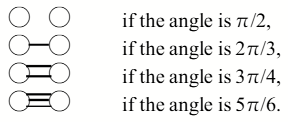
\includegraphics[width=0.4\linewidth]{Immagini - Capitolo 3/lines rule Dynkin diagrams.png}
    \caption{the relation between the number of lines and the angle between two roots in the Dynkin diagrams.}
    \label{fig: lines rule Dynkin diagrams}
\end{figure}
\begin{ex}
    There can be some degenerate diagrams. For example, the Dynkin diagram $\dynkin{C}{2}$ is the same for $C_2$ and $B_2$, this implies that the algebras associated are isomorphic, namely $\soa(6) \simeq \spa(4)$. The same happens for the diagram $\dynkin{D}{3}$ which is shared between $D_3$ and $A_3$, leading to $\soa(6) \simeq \sua(4)$. Instead, the diagram $\dynkin{D}{2}$ of $D_2$ can be written as the ``sum'' of two copies of $A_1$ diagrams $\dynkin{A}{1}$, leading to the relation $\soa(4) \simeq \sua(2) \op \sua(2)$.
\end{ex}
\begin{figure}[h]
    \centering
    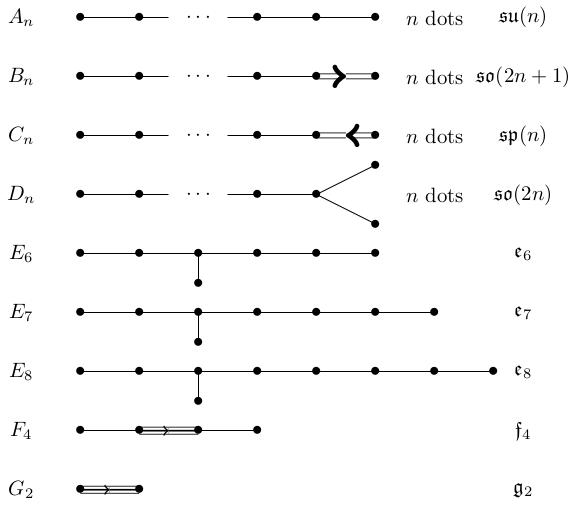
\includegraphics[width=0.5\linewidth]{Immagini - Capitolo 3/finite Dynkin diagrams.png}
    \caption{finite Dynkin diagrams of four infinite families, namely $A_n$, $B_n$, $C_n$ and $D_n$, and of five finite families, namely $g_2$, $f_4$, $e_6$, $e_7$ and $e_8$, with their associated Lie algebras.}
    \label{fig: finite Dynkin diagrams}
\end{figure}
Given an arbitrary irreducible representation $D$, one define a weight vector $\mu$ in $D$ as the highest weight in that representation if and only if, for every positive root $\phi$, the sum $\mu + \phi$ is not a weight in that representation. This is equivalent to requiring that $\mu + \alpha^i$ is not a weight for all simple roots $\alpha^i$. As a consequence, when $E_{\alpha^i}$ acts on $\mu$, the corresponding $p^i$ must be zero, namely equation $(\alpha \cdot \beta)/\alpha^2 = M/2$ must reduce to 
\begin{equation}
    \frac{2(\alpha^i \cdot \mu)}{(\alpha^i)^2} = q^i,\quad q^i \in \N.
\end{equation}
The latter equation can be interpreted as a relation giving the components of $\mu$ on the basis of the simple roots $\alpha^i$. Introducing the coroots of the simple roots by recalling equation \eqref{eq: coroot definition}, this equation can be written in a more concise form
\begin{equation}
    (\alpha^{i\vee},\mu) = q^i.
\end{equation}
Knowing the highest vector $\mu$, one can construct also the other vectors in that representation by acting on $\mu$ with the lowering operators $E_{-\alpha^i}$. This means that every irreducible representation of a simple Lie group of rank $m$ can be uniquely identified by the $m$ natural number $q^i$. It is particularly interesting to consider a set of $m$ irreducible representations $D^i$ with highest vectors $\mu^j$ such that
\begin{equation}
\label{eq: highest vector condition}
    \frac{2(\alpha^i \cdot \mu^j)}{(\alpha^i)^2} = \delta^{ij}.
\end{equation}
Each highest vector satisfying equation \eqref{eq: highest vector condition} is said to be a ``fundamental weight vector''. Using the definition of the coroots of the simple roots given in equation \eqref{eq: coroot definition}, the condition in \eqref{eq: highest vector condition} can be interpreted as an orthonormality relation relation 
\begin{equation}
    (\alpha^{i\vee},\mu^j) = \delta^{ij}.
\end{equation}
Each irreducible representation $D^j$ having a fundamental weight $\mu^j$ as highest vector is said to be a ``fundamental representation''. The fundamental weight provides a basis on which to expand the highest vector of every irreducible representation in a unique way
\begin{equation}
    \mu = \sum_{j=1}^m q^j\mu^j,\quad q^j \in \N.
\end{equation}
Alternatively, one can label the irreducible representation by just listing the integers $(q^1,\dots,q^m)$; this is called the Dynkin label of the representation. With this labelling, the fundamental representations have the labels $(1,0,\dots,0),\dots,(0,\dots,0,1)$.

\section{Lie algebra of SU(3)}
The $SU(3)$ Lie group is defined as the group of $3 \times 3$ complex unitary matrices $U$ having a unit determinant, with matrix multiplication as the group product. The dimension of the associated Lie algebra $\sua(3)$ is $\dim{\sua(3)} = 8$. The generators of $\sua(3)$ are eight Hermitian traceless matrices. A common choice for a defining representation is in terms of a basis given by the Gell-Mann matrices $\lambda_a$, which are the analogue of the Pauli matrices for the algebra of generators of the $SU(2)$ Lie group. The Gell-Mann matrices are
\begin{gather}
    \lambda_1 = 
    \begin{pmatrix}
        0 & 1 & 0 \\
        1 & 0 & 0 \\
        0 & 0 & 0
    \end{pmatrix},\quad 
    \lambda_2 = 
    \begin{pmatrix}
        0 & -i & 0 \\
        i & 0 & 0 \\
        0 & 0 & 0
    \end{pmatrix},\quad 
    \lambda_3 = 
    \begin{pmatrix}
        1 & 0 & 0 \\
        0 & -1 & 0 \\
        0 & 0 & 0
    \end{pmatrix}, \\ 
    \lambda_4 = 
    \begin{pmatrix}
        0 & 0 & 1 \\
        0 & 0 & 0 \\
        1 & 0 & 0
    \end{pmatrix},\quad
    \lambda_5 = 
    \begin{pmatrix}
        0 & 0 & -i \\
        0 & 0 & 0 \\
        i & 0 & 0
    \end{pmatrix},\quad 
    \lambda_6 = 
    \begin{pmatrix}
        0 & 0 & 0 \\
        0 & 0 & 1 \\
        0 & 1 & 0
    \end{pmatrix}, \\ 
    \lambda_7 = 
    \begin{pmatrix}
        0 & 0 & 0 \\
        0 & 0 & -i \\
        0 & i & 0
    \end{pmatrix},\quad 
    \lambda_8 = \frac{1}{\sqrt{3}} 
    \begin{pmatrix}
        1 & 0 & 0 \\
        0 & 1 & 0 \\
        0 & 0 & -2
    \end{pmatrix}.
\end{gather}
The generators $X_a$ of the $\sua(3)$ algebra are then 
\begin{equation}
\label{eq: su(3) algebra generators}
    X_a = \frac{\lambda_a}{2},\quad \forall a = \{1,\dots,8\}.
\end{equation}
The generators are normalised as
\begin{equation}
\label{eq: normalisation of su(3) algebra generators}
    \tr{(X_aX_b)} = \frac{\delta_{ab}}{2},\quad \forall a,b = \{1,\dots,8\},
\end{equation}
so the Dynkin index of the defining representation is 
\begin{equation}
\label{eq: Dynkin index of su(3) algebra defininf representation}
    \lambda_{def.} = \frac{1}{2}. 
\end{equation}
The rank of the $\sua(3)$ algebra is $m = 2$, so in the basis of generators $\{X_a\}$ the generators $X_3$ and $X_8$ are diagonal, thus they are Cartan generators. The often used convention is to name $H_1 \equiv X_3$ and $H_2 \equiv X_8$ as the $\sua(3)$ Cartan generators. Since they are diagonal, their common eigenvectors are
\begin{equation}
    e_1 = 
    \begin{pmatrix}
        1 \\
        0 \\
        0
    \end{pmatrix},\quad
    e_2 = 
    \begin{pmatrix}
        0 \\
        1 \\
        0
    \end{pmatrix},\quad
    e_3 = 
    \begin{pmatrix}
        0 \\
        0 \\
        1
    \end{pmatrix}.
\end{equation}
The eigenvalues of $H_1$ and $H_2$ are the weights $\mu_1$ and $\mu_2$, forming the weight vector $\mu = (\mu_1,\mu_2)$. Moving to the Dirac notation, the weights are used to label the eigenvectors, which are
\begin{equation}
    e_1 = \bigket{\frac{1}{2},\frac{1}{2\sqrt{3}}},\quad e_2 = \bigket{-\frac{1}{2},\frac{1}{2\sqrt{3}}},\quad e_3 = \bigket{0,-\frac{1}{\sqrt{3}}}.
\end{equation}
If one plots the weight vector on the $(\mu_1,\mu_2)$ plane, they form an equilateral triangle, as shown in figure \ref{fig: fundamental and anti-fundamental representation of su(3)}. 
\begin{figure}[h]
    \centering
    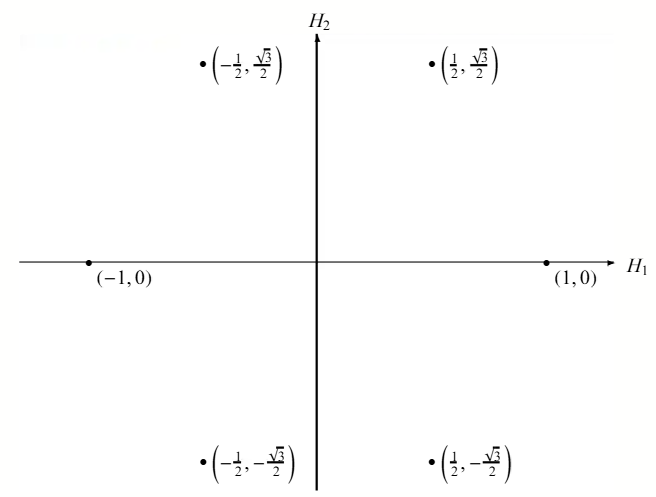
\includegraphics[width=0.55\linewidth]{Immagini - Capitolo 3/roots of su(3).png}
    \caption{roots of the $\sua(3)$.}
    \label{fig: roots of su(3)}
\end{figure}

There will be $8 - 2 = 6$ root vectors, namely three pairs $\pm\alpha$. To find them, one can use the fact that the corresponding generators $E_{\pm\alpha}$ map weights in to one another. Thus, the $\alpha$ vectors are found as differences of weights. In the plot of the weight vectors on the $(\mu_1,\mu_2)$ plane, they correspond to the vectors from one weight to another. Thus, it is simple to read off that the possible $\alpha$ vectors are
\begin{equation}
    \alpha \in \bigg\{ \pm(1,0),\quad \pm\bigg(\frac{1}{2},\frac{\sqrt{3}}{2}\bigg),\quad \pm\bigg(-\frac{1}{2},\frac{\sqrt{3}}{2}\bigg) \bigg\}.
\end{equation}
The roots form a regular hexagon, centred at the origin of the $(H_1,H_2)$ plane, as shown in figure \ref{fig: roots of su(3)}. Note also that all angles between root vectors of the $\sua(3)$ algebra are multiples of $\pi/3$. 
\begin{figure}[H]
    \centering
    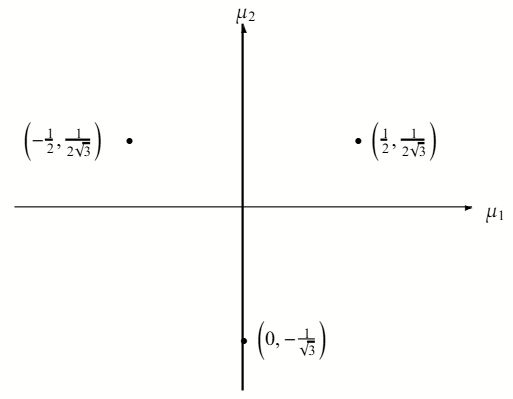
\includegraphics[width=0.44\linewidth]{Immagini - Capitolo 3/fundamental representation.png}
    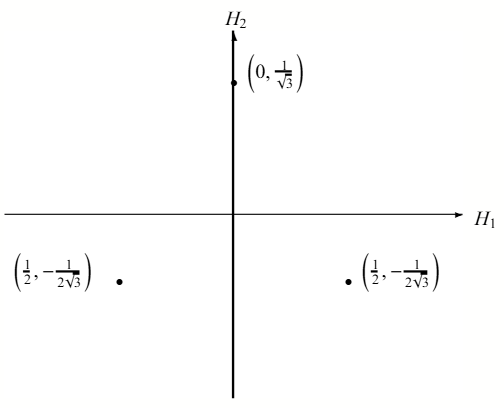
\includegraphics[width=0.42\linewidth]{Immagini - Capitolo 3/anti-fundamental representation.png}
    \caption{roots of the $\sua(3)$: (i) $\bm{3}$ fundamental representation; (ii) $\bar{\bm{3}}$ anti-fundamental representation.}
    \label{fig: fundamental and anti-fundamental representation of su(3)}
\end{figure}

In the defining representation of the $\sua(3)$ Lie algebra one can easily see that the highest weight $\ket{1/2,1/2\sqrt{3}}$ is not the lowest one $\ket{-1/2,1/2\sqrt{3}}$ with a minus sign. Thus, the $\sua(3)$ defining representation is a complex one. In Physics, it is customary to denote the defining representation as the ``fundamental representation'' and it is denoted by $\bm{3}$. Its complex conjugate representation is denoted ad $\bar{\bm{3}}$ and it is called the ``anti-fundamental representation'', with highest weight $\ket{1/2,-1/2\sqrt{3}}$; its weights are equal and opposite to those of the fundamental representation, and are shown again in figure \ref{fig: fundamental and anti-fundamental representation of su(3)}.

\section{Young diagrams for \texorpdfstring{$SU(N)$}{SU(N)}}
A generic irreducible representation $D$ of $SU(N)$ has the highest weight vector $\mu$, which can be expanded over the $N - 1$ fundamental weights $\mu^k$ as
\begin{equation}
    \mu = q^1\mu^1 + \cdots + q^{N-1}\mu^{N-1},
\end{equation}
so that alternatively one can specify $D$ with the Dynkin label $(q^1,\dots,q^{N-1})$. The irreducible representation $D$ can be associated with a Young diagram with $q^k$ columns of $k$ boxes, for $k = 1,\dots,N-1$, as shown below.
\ytableausetup{mathmode, boxframe=normal, boxsize=2.2em}
\begin{equation}
    \raisebox{8ex}{
        \begin{ytableau}
        1 & \cdots & \scriptstyle q^{N-1} & 1 & \cdots & 1 & \cdots & \scriptstyle q^2 & 1 & \cdots & \scriptstyle q^1 \\
        1 & \cdots & \scriptstyle q^{N-1} & 1 & \cdots & 1 & \cdots & \scriptstyle q^2 \\
        \none[\vdots] & \none[\vdots] & \none[\vdots] & \none[\vdots] & \none[\vdots] & \none[\vdots] \\
        1 & \cdots & \scriptstyle q^{N-1} & 1 & \cdots & \scriptstyle q^{N-2} \\
        1 & \cdots & \scriptstyle q^{N-1}
    \end{ytableau}
    }
\end{equation}
Alternatively, one could label the diagram by the number of boxes in each row; in the $k$th row there are $l_k$ boxes, with
\begin{equation}
    \begin{cases}
        l_1 = q^{N-1} + q^{N-2} + \cdots + q^2 + q^1 \\
        l_2 = q^{N-1} + q^{N-2} + \cdots + q^2 \\
        \vdots \\
        l_{N-1} = q^{N-1}
    \end{cases}.
\end{equation}
The table is now labelled by the list $\{l_1,\dots,l_{N-1}\}$, sometimes called the partition, resulting in the diagram below.
\begin{equation}
    \raisebox{0ex}{
        \begin{ytableau}
        1 & \cdots & \scriptstyle l_{N-1} & \cdots & \cdots & \scriptstyle l_{N-2} & \cdots & \scriptstyle l_3 & \cdots & \scriptstyle l_2 & \scriptstyle l_2 + 1 & \cdots & \scriptstyle l_1 \\
                1 & \cdots & \scriptstyle l_{N-1} & \cdots & \cdots & \scriptstyle \scriptstyle l_{N-2} & \cdots & \scriptstyle l_3 & \cdots & \scriptstyle l_2 \\
        \none[\vdots] & \none[\vdots] & \none[\vdots] & \none[\vdots] & \none[\vdots] & \none[\vdots] \\
        1 & \cdots & \scriptstyle l_{N-1} & \cdots & \cdots & \scriptstyle l_{N-2} \\
        1 & \cdots & \scriptstyle l_{N-1}
    \end{ytableau}
    }
\end{equation}
The dimension of the irreducible representation can be computed from its Young diagram using the factors-over-hooks rule. The rule works as follows. For an $\sua(N)$ diagram, put integers into boxes starting from the top-left corner, where the number $N$ is put. Then fill in the first row, increasing integers by one at each step to the right. For the second row, start from the left with $N - 1$, then fill the row, increasing the integers by one at each step. This goes on until all boxes in the diagram are filled. Then one computes the product of all the integers in the boxes, thus computing the number of factors, denoted as $F$. Moreover, a hook is a set of boxes with a shape like the $\neg$ symbol, that starts from the last box in a row, goes left and then turns down at some point, and continues down through the end of the column below. For each hook $i$, calculate the hook factor $h_i$, which is the number of boxes that the hook passes through. Then one calculates the product $H = \prod_ih_i$ over all hooks. The dimension of the representation is then the ratio
\begin{equation}
    \dim{D} = \frac{F}{H}.
\end{equation}
Consider now the tensor product of two irreducible representations $A \ot B$, using the corresponding Young diagrams. The process to compute this operation follows the general rules: 
\begin{enumerate}
    \item Put letters $a$ in the boxes on the first row of the diagram for $B$, letters $b$ in the second row, letters c in the third row, and so on, for example
    \begin{equation}
    \ytableausetup{mathmode, boxframe=normal, boxsize=1.3em}
    \raisebox{4ex}{
        \begin{ytableau}
        a & a & a & a \\
        b & b & b \\
        c \\
        d
        \end{ytableau}
        };
    \end{equation}
    \item take boxes with $a$ from $B$ and attach them in all possible ways to the ends of the rows of $A$ to get an expanded diagram, such that there is no more than one box with $a$ in each column of the expanded diagram $A$ (there can be more than one a per row);
    \item take the boxes with $b$ from $B$ and attach them to the previously obtained expanded diagram $A$, again enforcing that there is no more than one $b$ per column;
    \item take the boxes with $c$ from $B$ and attach them to the previously obtained expanded diagram $A$, again with the same rule, so that there is no more than one $c$ per column;
    \item repeat this procedure until all the letters have been used;
    \item for every diagram, form a word as follows: 
    \begin{enumerate}[i.]
        \item start reading the first row from right to left, at every step, add the letter that you encounter to the end of the word;
        \item after finishing the first row, move to the second row and repeat the process row by row and read from right to left adding letters to the word.
    \end{enumerate}
    \item generalize the previous definition of an admissible word if, by reading it from left to right, at every step at least as many $a$s have occurred as $b$s, $c$s, and so on, up to that point, at least as many $b$s have occurred as $c$s, $d$s, and so on, up to that point, and so on and so forth, for example $aabc$ and $ababc$ are admissible words, while $acba$ and $bca$ are not;
    \item discard the diagrams with non-admissible words, the remaining ones form the decomposition of the tensor product;
    \item identify every diagram as a $(q^1,\dots,q^{N-1})$ irreducible representation;
    \item compute their dimensions using the factors-over-hooks rule.
\end{enumerate}
\begin{ex}
    As an example, consider the decomposition of the tensor product of the adjoint representation $\bm{8}$ of the $\sua(3)$ algebra with itself, namely
    \begin{equation}
        \bm{8} \ot \bm{8} = \ydiagram{2,1} \ot \ytableaushort{aa,b}\,.
    \end{equation}
    So, following the rules, the first step leads to the diagrams
    \begin{equation}
        \ytableaushort{{}{}aa,{}}
        \,,\quad
        \ytableaushort{{}{}a,{}a}
        \,,\quad
        \ytableaushort{{}{}a,{},a}
        \,,\quad
        \ytableaushort{{}{},{}a,a}\,.
    \end{equation}
    Now, the process is repeated for the letter $b$, resulting in the diagrams
    \begin{gather}
        \cancel{\ytableaushort{{}{}aab,{}}}
        \,,\quad
        \ytableaushort{{}{}aa,{}b}
        \,,\quad
        \ytableaushort{{}{}aa,{},b}
        \,,\quad
        \cancel{\ytableaushort{{}{}ab,{}a}}
        \,, \\
        \ytableaushort{{}{}a,{}ab}
        \,,\quad
        \ytableaushort{{}{}a,{}a,b}
        \,,\quad
        \cancel{\ytableaushort{{}{}ab,{},a}}
        \,,\quad
        \ytableaushort{{}{}b,{}a,a}
        \,,\quad
        \ytableaushort{{}{},{}a,ab}
        \,.
    \end{gather}
    Thus, the decomposition is given by
    \begin{multline}
        \ytableaushort{{}{}aa,{}b} \op \ytableaushort{{}{}aa,{},b} \op \ytableaushort{{}{}a,{}ab} \op \ytableaushort{{}{}a,{}a,b}\, \op \\
        \op \ytableaushort{{}{}b,{}a,a} \op \ytableaushort{{}{},{}a,ab} = \ydiagram{4,2} \op \ydiagram{3}\, \op \\ \op \ydiagram{3,3} \op \ydiagram{2,1} \op \ydiagram{2,1} \op \bullet,
    \end{multline}
    or in a more compact notation
    \begin{multline}
        (2,2) \op (3,0) \op (0,3) \op (1,1) \op (1,1) \op (0,0) = \\ = \bm{27} \op \bm{10} \op \bar{\bm{10}} \op \bm{8} \op \bm{8} \op \bm{1}.
    \end{multline}
    Note that four diagrams were discarded with the non-admissible word $baa$ and were kept the six diagrams with the admissible words $aab$, $aab$, $aba$, $aab$, $aba$ and $aba$.
\end{ex}
\begin{ex}
    Consider the tensor product of the fundamental representation $\bm{3}$ with the antifundamental one $\bar{\bm{3}}$. Using again the set of rules for the product
    \begin{equation}
        \bm{3} \ot \bar{\bm{3}} = \ydiagram{1} \ot \ytableaushort{a,b}\,,
    \end{equation}
    gives two possibilities for the letter $a$, namely 
    \begin{equation}
        \ytableaushort{{}a}\,,\quad \ytableaushort{{},a}\,.
    \end{equation}
    Now, passing over to the letter $b$ the diagrams in the first case are
    \begin{equation}
        \cancel{\ytableaushort{{}{}ab}}\,,\quad \ytableaushort{{}a,b}\,,
    \end{equation}
    while in the second one are
    \begin{equation}
        \cancel{\ytableaushort{{}b,a}}\,,\quad \ytableaushort{{},a,b} = \ydiagram{2,1} \op \bullet.
    \end{equation}
    Thus, the decomposition is
    \begin{equation}
        \bm{3} \ot \bar{\bm{3}} = (1,1) \op (0,0) = \bm{8} \op \bm{1}.
    \end{equation}
    As a rule of thumb, it turns out that, in the $A \ot B$ product, it is generally convenient to take $B$ to be the representation with the simpler of the two Young diagrams; recall that, although the tensor product is not a commutative operation, $A \ot B$ and $B \ot A$ are equivalent up to a redefinition of the order of rows and columns, hence the two representations $A \ot B$ and $B \ot A$ are unitarily equivalent. In this regard, consider the tensor product $\bar{\bm{3}} \ot \bm{3}$, using the same rules on
    \begin{equation}
        \bar{\bm{3}} \ot \bm{3} = \ydiagram{1,1} \ot \ytableaushort{a}
    \end{equation}
    one has the diagrams
    \begin{equation}
        \ytableaushort{{}a,{}}\,,\quad \ytableaushort{{},{},a} = (1,1) \op (0,0),
    \end{equation}
    thus the decomposition, as expected, is the same found for the $\bm{3} \ot \bar{\bm{3}}$, namely $\bar{\bm{3}} \ot \bm{3} = \bm{8} \op \bm{1}$.
\end{ex}
\begin{ex}
    Consider the tensor product between the following two representations of the $\sua(4)$ algebra
    \begin{equation}
        \ydiagram{1,1} \ot \ytableaushort{a,b,c}\,,
    \end{equation}
    whose dimension is equal to 24 since the dimensions of the single representations, using the factors-over-hooks rule, are
    \begin{equation}
        \dim\left(\,\vcenter{\hbox{\ydiagram{1,1}}}\,\right) = 6,\quad \dim\left(\,\vcenter{\hbox{\ydiagram{1,1,1}}}\,\right) = 4.
    \end{equation}
    For the first letter there are only two possibilities
    \begin{equation}
        \ytableaushort{{}a,{}}\,,\quad \ytableaushort{{},{},a}\,.
    \end{equation}
    Passing over to the second letter $b$ the number of diagrams grows to
    \begin{equation}
        \ytableaushort{{}ab,{}}\,,\quad \ytableaushort{{}a,{}b}\,,\quad \ytableaushort{{}a,{},b}\,,\quad \ytableaushort{{}b,{},a}\,,\quad \ytableaushort{{},{},a,b}\,.
    \end{equation}
    Then, considering the last letter, the total number of diagrams consist in
    \begin{gather}
        \ytableaushort{{}ab,{}c}\,,\quad \ytableaushort{{}abc,{}}\,,\quad \ytableaushort{{}ab,{},c}\,,\quad \ytableaushort{{}ac,{}b}\,,\quad \ytableaushort{{}a,{}b,c} \\
        \ytableaushort{{}ac,{}b}\,,\quad \ytableaushort{{}a,{},b,c}\,,\quad \ytableaushort{{}bc,{},a}\,,\quad \ytableaushort{{}c,{},a,b}\,,\quad \ytableaushort{{},{},a,b,c}\,.
    \end{gather}
    Now removing the non-admissible diagrams the tensor product in question results in 
    \begin{equation}
        \ydiagram{1,1} \ot \ydiagram{1,1,1} = \ydiagram{2,2,1} \op \ydiagram{2,1,1,1} = \ydiagram{2,2,1} \op \ydiagram{1}\,.
    \end{equation}
    To check if the tensor product result is coherent, one can compute the dimensions of the diagrams obtained, which in this case are
    \begin{equation}
        \dim\left(\,\vcenter{\hbox{\ydiagram{2,2,1}}}\,\right) = 20,\quad \dim\left(\,\vcenter{\hbox{\ydiagram{1}}}\,\right) = 4,
    \end{equation}
    whose sum is 24 as expected.
\end{ex}

\section{Lorentz group}
The Lorentz group is the group of transformations of spacetime coordinate in special relativity relating quantities measured by different observers in motion at constant speed with respect to each other, in other words by observers in different inertial frames of reference. Special relativity is based on two postulates:
\begin{enumerate}
    \item all physical laws have the same form in all inertial frames;
    \item the speed of light in a vacuum is the same in all inertial frames.
\end{enumerate}
Consider two inertial reference frames with spacetime coordinates $x^\mu = (t,x^1,x^2,x^3)$ and $x'^\mu = (t,x'^1,x'^2,x'^3)$ and assume that at $t = t' = 0$ the two frames coincide, namely $x^\mu(t = 0) = x'^\mu(t' = 0)$. Then, according to the second postulate of special relativity, a ray of light emitted at the origin at that time ans propagating to another point $P$ at a later time should be such that the spacetime coordinated of $P$ measured in the two inertial frames satisfy
\begin{equation}
    (ct)^2 - x_ix^i = (ct')^2 - x_i'x'^i.
\end{equation}
Introducing the Minkowski metric $g_{\mu\nu}$ as the matrix\footnote{One can also define the Minkowski metric as $g_{\mu\nu} = \mathrm{diag}(-1,1,1,1)$, which is often used in spacial and general relativity, but usually the convention in particle physics is given by equation \eqref{eq: Minkowski metric definition}; either way the results obtained through them are equivalent.}
\begin{equation}
\label{eq: Minkowski metric definition}
    g_{\mu\nu} = 
    \begin{pmatrix}
        1 & 0 & 0 & 0 \\
        0 & - 1 & 0 & 0 \\
        0 & 0 & -1 & 0 \\
        0 & 0 & 0 & -1
    \end{pmatrix},
\end{equation}
the latter equation can be written as
\begin{equation}
\label{eq: invariance of relativistic interval}
    g_{\mu\nu}x^\mu x^\nu = g_{\mu\nu}x'^\mu x'^\nu.
\end{equation}
In special relativity, an event is defined as a point in spacetime, so given two events $A$ and $B$, on can define the squared relativistic interval $\Delta s_{AB}^2$ as
\begin{equation}
    \Delta s_{AB}^2 = (x_A^0 - x_B^0)^2 - (x_A^i - x_B^i)^2 = g_{\mu\nu}(x_A - x_B)^\mu(x_A - x_B)^\nu,
\end{equation}
and this quantity is an example of a relativistic invariant, namely a quantity that has the property to have the same value in all inertial frames. Assuming that the spacetime coordinates of an event expressed in two different inertial frames, $x^\alpha$ and $x^\beta$, are related to each other by a set of linear transformations
\begin{equation}
\label{eq: Lorentz transformation}
    x'^\beta = \Lambda^\beta_\alpha x^\alpha.
\end{equation}
Furthermore, equation \eqref{eq: invariance of relativistic interval} implies that 
\begin{equation}
    g_{\mu\nu}x^\mu x^\nu = g_{\alpha\beta}\Lambda^\alpha_\mu \Lambda^\nu_\beta x^\mu x^\nu,
\end{equation}
and since this must hold for every arbitrary $x^\mu$ it follows that
\begin{equation}
\label{eq: RS principle}
    g_{\mu\nu} = g_{\alpha\beta}\Lambda^\alpha_\mu \Lambda^\nu_\beta.
\end{equation}
A spacetime coordinate transformation $\Lambda$ which satisfies equation \eqref{eq: RS principle} is called a Lorentz transformation. Consider the $\mu = \nu = 0$ component of again equation \eqref{eq: RS principle}, that is 
\begin{equation}
    1 = g_{\alpha\beta}\Lambda^\alpha_0 \Lambda^\nu_0 = (\Lambda_0^0)^2 - (\Lambda_0^i)^2,
\end{equation}
from which one deduces that
\begin{equation}
    |\Lambda^0_0| = \sqrt{1 + (\Lambda_0^i)^2} \ge 1.
\end{equation}
Depending on the sign of $\Lambda_0^0$, the transformation represented by the $\Lambda$ matrix is said to be:
\begin{enumerate}
    \item an orthochronous Lorentz transformation if $\Lambda_0^0 \ge 1$;
    \item an antichronous Lorentz transformation if $\Lambda_0^0 \le -1$.
\end{enumerate}
Moreover, if one interprets $x^\mu$ and $x'^\mu$ coordinates as four-component, real-valued column vectors, and $g$ and $\Lambda$ as $4 \times 4$ real-valued matrices, then equation \eqref{eq: RS principle} can be thought of as the matrix relation 
\begin{equation}
\label{eq: RS principle in matrix form}
    g = \Lambda^Tg\Lambda.
\end{equation}
Taking the determinant of equation \eqref{eq: RS principle in matrix form}, one deduces that $\det{\Lambda} = \pm1$. Accordingly, one distinguishes:
\begin{enumerate}
    \item a proper Lorentz transformation if $\det{\Lambda} = 1$;
    \item an improper Lorentz transformation if $\det{\Lambda} = -1$;
\end{enumerate}
One can note that equation \eqref{eq: RS principle in matrix form} has an analogy with the one that characterises the group of orthogonal transformation of size four, denoted as $O(4)$, namely $\MI_4 = O^T\MI_4O$, the difference being that $\MI_{\mu\nu} = \delta_{\mu\nu}$ while $g_{\mu\nu}$ is defined as in equation \eqref{eq: Minkowski metric definition}. To stress the fact that three diagonal entries of $g_{\mu\nu}$ have the same sign, while one has the opposite sign, the set of matrices satisfying equation \eqref{eq: RS principle in matrix form} is denoted as $O(3,1)$. These matrices, with the matrix row-by-column multiplication as the group product, form a group called the Lorentz group. This group can be defined as the set of coordinate transformation leaving the $\Delta s^2$ invariant. Furthermore, while $x_\mu x^\mu$ is always non-negative and it is zero if and only if $x^\mu = 0$, the invariant $\Delta s^2$ can be either positive, zero or negative. Accordingly, a four-vector $x^\mu$ is said to be:
\begin{enumerate}
    \item a timelike four-vector if $(x^0)^2 - (x^i)^2 > 0$;
    \item a lightlike four-vector if $(x^0)^2 - (x^i)^2 = 0$;
    \item a spacelike four-vector if $(x^0)^2 - (x^i)^2 < 0$.
\end{enumerate}

\subsubsection{Rotations}
Matrices of the form 
\begin{equation}
\label{eq: general Lorentz rotation}
    \Lambda = 
    \begin{pmatrix}
        1 & 0 & 0 & 0 \\
        0 & & & \\
        0 & & R & \\
        0 & & &
    \end{pmatrix},\quad R \in O(3),
\end{equation}
describe transformations that leave the $x^0$ coordinate unchanged, and rotate the spatial axes of the reference frames; the transformation is an orthochronus Lorentz transformation and it is proper if $\det{R} = 1$, namely if $R \in SO(3)$. Note that the inverse transformation $\Lambda^{-1}$ has the same for as $\Lambda$, but with $R$ replaced with $R^T$. 

As a particular case of equation \eqref{eq: general Lorentz rotation}, a rotation of the reference frame by an angle $\theta$ around the $z$-axis takes the form 
\begin{equation}
    \Lambda =
    \begin{pmatrix}
        1 & 0 & 0 & 0 \\
        0 & \cos{\theta} & \sin{\theta} & 0 \\
        0 & -\sin{\theta} & \cos{\theta} & 0 \\
        0 & 0 & 0 & 1
    \end{pmatrix}.
\end{equation}
When the angle $\theta$ is infinitesimally small, one can expand around the unit element
\begin{equation}
    \Lambda =
    \begin{pmatrix}
        1 & 0 & 0 & 0 \\
        0 & 1 & \theta & 0 \\
        0 & -\theta & 1 & 0 \\
        0 & 0 & 0 & 1
    \end{pmatrix} = \MI_4 +i\theta
    \begin{pmatrix}
        0 & 0 & 0 & 0 \\
        0 & 0 & -i & 0 \\
        0 & i & 0 & 0 \\
        0 & 0 & 0 & 0
    \end{pmatrix} + o(\theta^2)
\end{equation}
from which one can read off the generator of rotations around the $z$-axis as the matrix multiplied by $i\theta$ in the last term. With a similar argument, one can derive the generators of rotations around the other two spatial axes, finding
\begin{equation}
    J^1 = 
    \begin{pmatrix}
        0 & 0 & 0 & 0 \\
        0 & 0 & 0 & 0 \\
        0 & 0 & 0 & -i \\
        0 & 0 & i & 0
    \end{pmatrix},\quad
    J^2 = 
    \begin{pmatrix}
        0 & 0 & 0 & 0 \\
        0 & 0 & 0 & i \\
        0 & 0 & 0 & 0 \\
        0 &-i & 0 & 0
    \end{pmatrix},\quad
    J^3 = 
    \begin{pmatrix}
        0 & 0 & 0 & 0 \\
        0 & 0 & -i & 0 \\
        0 & i & 0 & 0 \\
        0 & 0 & 0 & 0
    \end{pmatrix}
\end{equation}
which form an $\sua(2)$ algebra since they satisfy the commutation relation
\begin{equation}
    \comm{J^a}{J^b} = i\epsilon_{abc}J^c.
\end{equation}

Another particular case of equation \eqref{eq: general Lorentz rotation} is the parity transformation, namely the inversion of all spatial coordinates, corresponding to imposing $R = -\MI_3$ in said equation, which is a improper orthochronus Lorentz transformation. Note that the parity transformation does not depend on a continuous parameter, because of that it is a discrete transformation. Furthermore, parity transformation is such that its square equals the identity, hence it is equal to its inverse.

\subsubsection{Boosts}
Relativistic transformations of the spacetime coordinates between two inertial reference frames moving at constant relative velocity of modulus $v$ are called Lorentz boosts; in the particular case where the reference frame with coordinates $x'^\mu$ is moving with respect to the reference frame with coordinates $x^\mu$ at velocity $v$ along the $x$-direction then the boost can be represented by the matrix
\begin{equation}
    \Lambda = 
    \begin{pmatrix}
        \gamma & -\beta\gamma & 0 & 0 \\
        -\beta\gamma & \gamma & 0 & 0 \\
        0 & 0 & 0 & 0 \\
        0 & 0 & 0 & 0
    \end{pmatrix},
\end{equation}
that by defining the rapidity $\eta = \arcsinh{(\beta\gamma)}$ can be also written as
\begin{equation}
\label{eq: Lorentz boost along x-axis (rapidity)}
    \Lambda = 
    \begin{pmatrix}
        \cosh{\eta} & -\sinh{\eta} & 0 & 0 \\
        -\sinh{\eta} & \cosh{\eta} & 0 & 0 \\
        0 & 0 & 1 & 0 \\
        0 & 0 & 0 & 1
    \end{pmatrix}.
\end{equation}
In order to give a proper definition of infinitesimal boosts, recall first that the condition that defines a Lorentz transformation is $g_{\mu\nu} = g_{\alpha\beta}\Lambda^\alpha_\mu\Lambda^\beta_\nu = \Lambda_{\beta\mu}\Lambda^\beta_\nu$; when $\Lambda$ is a proper and orthochronus Lorentz trasformation infinitesimally close to the identity, one can write
\begin{equation}
    \Lambda^\alpha_\mu = g^\alpha_\mu + \omega^\alpha_\mu,
\end{equation}
where the components of $\omega$ are infinitesimally small, so that one has
\begin{equation}
    g_{\mu\nu} = \Lambda_{\beta\mu}\Lambda^\beta_\nu \simeq (g_{\beta\mu} + \omega_{\beta\mu})(g^\beta_\nu + \omega^\beta_\nu) = g_{\mu\nu} + \omega_{\mu\nu} + \omega_{\nu\mu},
\end{equation}
from which the following condition is obtained
\begin{equation}
    \omega_{\mu\nu} = - \omega_{\nu\mu}.
\end{equation}
Now, consider again the matrix in equation \eqref{eq: Lorentz boost along x-axis (rapidity)} in the limit where $\eta$ is infinitesimally small, then
\begin{equation}
    \Lambda = 
    \begin{pmatrix}
        1 & -\eta & 0 & 0 \\
        -\eta & 1 & 0 & 0 \\
        0 & 0 & 1 & 0 \\
        0 & 0 & 0 & 1 \\
    \end{pmatrix} = \MI_4 + i\eta
    \begin{pmatrix}
        0 & i & 0 & 0 \\
        i & 0 & 0 & 0 \\
        0 & 0 & 0 & 0 \\
        0 & 0 & 0 & 0 \\
    \end{pmatrix} + o(\eta^2)
\end{equation}
from which one can read off the generator of Lorentz boosts along the $x$-axis as the matrix multiplied by the $i\eta$ in the last term. With a similar argument, one can derive the generators of Lorentz boosts along the other two spatial axes, finding 
\begin{equation}
    K^1 = 
    \begin{pmatrix}
        0 & i & 0 & 0 \\
        i & 0 & 0 & 0 \\
        0 & 0 & 0 & 0 \\
        0 & 0 & 0 & 0
    \end{pmatrix},\quad
    K^2 = 
    \begin{pmatrix}
        0 & 0 & i & 0 \\
        0 & 0 & 0 & 0 \\
        i & 0 & 0 & 0 \\
        0 & 0 & 0 & 0
    \end{pmatrix},\quad
    K^3 = 
    \begin{pmatrix}
        0 & 0 & 0 & i \\
        0 & 0 & 0 & 0 \\
        0 & 0 & 0 & 0 \\
        i & 0 & 0 & 0
    \end{pmatrix}.
\end{equation}
Note that the $K^a$ generators are anti-Hermitian. Anyway, in contrast to the generators of rotations, the boosts generators do not form a closed subalgebra themselves; instead
\begin{equation}
\label{eq: commutator between K and K}
    \comm{K^a}{K^b} = -i\epsilon_{abc}J^c.
\end{equation}
Moreover, the commutator of a rotation generator and a boost generator reads
\begin{equation}
\label{eq: commutator between J and K}
    \comm{J^a}{K^b} = i\epsilon_{abc}K^c.
\end{equation}

\subsubsection{Time inversion}
The Lorentz transformation described by the matrix 
\begin{equation}
    \Lambda = 
    \begin{pmatrix}
        -1 & 0 & 0 & 0 \\
        0 & 1 & 0 & 0 \\
        0 & 0 & 1 & 0 \\
        0 & 0 & 0 & 1
    \end{pmatrix}
\end{equation}
is an improper non-orthochronus Lorentz transformation that reverses the sign of time, leaving the spatial coordinates, as well as the $\Delta s^2$ invariant, unchanged. Like the parity transformation, the time inversion is a discrete transformation which squares the identity and, hence, equals its inverse.

\subsection{Lorentz group algebra}
While the relations \eqref{eq: commutator between K and K} and \eqref{eq: commutator between J and K} imply that generators of rotations and the generators of boosts do not form separate algebras, one can prove that, defining the following combinations of generators 
\begin{equation}
    N^a = \frac{1}{2}(J^a + iK^a),\quad M^a = \frac{1}{2}(J^a - iK^a),
\end{equation}
one obtains the two independent $\sua(2)$ algebras
\begin{equation}
    \comm{N^a}{N^b} = i\epsilon_{abc}N^c,\quad \comm{M^a}{M^b} = i\epsilon_{abc}M^c,\quad \comm{N^a}{M^b} = 0.
\end{equation}
Accordingly, the irreducible representations of the Lorentz group can be labelled by the labels of these two $\sua(2)$ subalgebras $(p,q)$ where $p$ and $q$ are integers or half-integers non-negative numbers related to the quadratic Casimir operator constructed from the $N^a$ and the $M^a$ generators as
\begin{equation}
    N_aN^a = p(p + 1)\MI_4,\quad M_aM^a = q(q + 1)\MI_4.
\end{equation}
Restrict now the discussion to the subset of continuos proper orthochronus Lorentz transformations, namely rotations and boosts. As discussed previously, they depend on six parameters, in particular three rotation angles and three components of the boost velocity. Consider then a Lorentz transformation that is infinitesimally close to the identity
\begin{equation}
\label{eq: infinitesimal Lorentz transformation}
    \Lambda^\beta_\alpha = \delta^\beta_\alpha + \epsilon^\beta_\alpha + o(\epsilon^2),
\end{equation}
that substituted in equation \eqref{eq: RS principle} gives
\begin{equation}
    \begin{split}
        g_{\mu\nu} &= g_{\alpha\beta}[\delta^\beta_\mu + \epsilon^\beta_\mu + o(\epsilon^2)][\delta^\beta_\nu + \epsilon^\beta_\nu + o(\epsilon^2)] \\
        &= g_{\alpha\beta}[\delta^\alpha_\mu\delta^\beta_\nu + \epsilon^\alpha_\mu\delta^\beta_\nu + \delta^\alpha_\mu\epsilon^\beta_\nu + o(\epsilon^2)] \\
        &= g_{\mu\nu} + \epsilon_{\nu\mu} + \epsilon_{\mu\nu} + o(\epsilon^2),
    \end{split}
\end{equation}
from which it follows the above found relation $\epsilon_{\mu\nu} = -\epsilon_{\nu\mu}$, implying that the infinitesimal generator of Lorentz transformations can be thought of as an antisymmetric $4 \times 4$ tensor with six independent components. Consider now the differential operator defined as
\begin{equation}
    L_{\mu\nu} = ix_\mu\frac{\p}{\p x^\nu} - ix_\nu\frac{\p}{\p x^\mu} \equiv i(x_\mu\p_\nu - x_\nu\p_\mu),
\end{equation}
they satisfy the Lorentz algebra
\begin{equation}
    \comm{L^{\alpha\beta}}{L^{\gamma\delta}} = i(g^{\beta\gamma}L^{\alpha\delta} + g^{\alpha\delta}L^{\beta\gamma} - g^{\beta\delta}L^{\alpha\gamma} - g^{\alpha\gamma}L^{\beta\delta})
\end{equation}
and allow one to write the variation of $x^\nu$ under an infinitesimal Lorentz transformation as
\begin{equation}
    \delta x^\nu = \frac{i}{2}\epsilon^{\alpha\beta}L_{\alpha\beta} x^\nu.
\end{equation}
For a Lorentz transformation that can be expressed as in equation \eqref{eq: infinitesimal Lorentz transformation}, one can thus define the operator
\begin{equation}
    U(\Lambda) = \exp{\bigg(\frac{i}{2}\epsilon^{\alpha\beta}L_{\alpha\beta}\bigg)},
\end{equation}
which can be used to classify the different type of fields based on their transformation properties under a Lorentz transformation. These transformations properties must account for the nature of the field and for the fact that it depends on spacetime coordinates which are not invariant under Lorentz transformations; for example, a scalar field $\phi(x)$ transforms as
\begin{equation}
    \phi(x') = U(\Lambda)\phi(x)U^{-1}(\Lambda),
\end{equation}
while a vector field $\phi^\alpha(x)$ transforms as
\begin{equation}
    \phi^\beta(x') = \Lambda^\beta_\alpha[U(\Lambda)\phi^\alpha(x)U^{-1}(\Lambda)].
\end{equation}
In fact, there could be many more types of fields, which could be constructed, for example, by considering the representation of the $\sua(2)$ algebras generated by the $N^a$and $N^{a\dg}$, that one can denote as $\bm{(p,q)}$, and their product. For instance:
\begin{enumerate}
    \item $\bm{(0,0)}$ corresponds to a scalar field;
    \item $\bm{(1/2,0)}$ corresponds to a left-handed, spin-half field;
    \item $\bm{(0,1/2)}$ corresponds to a right-handed, spin-half field;
    \item the product $\bm{(1/2,0)} \ot \bm{(0,1/2)} = \bm{(1/2,1/2)}$ corresponds to a spin-one vector field;
    \item the product $\bm{(1/2,0)} \ot \bm{(1/2,0)} = \bm{(0,0)} \op \bm{(1,0)}$ corresponds to a scalar representation times a two-index, antisymmetric, self-dual tensor;
    \item the product $\bm{(0,1/2)} \ot \bm{(0,1/2)} = \bm{(0,0)} \op \bm{(0,1)}$ corresponds to a scalar representation times a two-index, antisymmetric, anti-self-dual tensor.
\end{enumerate}
\begin{obs}
    The field strength tensor of electromagnetism is a physical example of a field transforming in the $\bm{(1,0)} \op \bm{(0,1)}$ representation of the Lorentz group.
\end{obs}

\section{Lorentz-Poincaré group}
As discussed above, the Lorentz group consists of the linear coordinate transformation that are consistent with the principles of special relativity theory. However, as the physical laws depend only on differences of physical coordinates, one can extend the set of coordinate transformations to include also spacetime translations, generalising equation \eqref{eq: Lorentz transformation} to
\begin{equation}
\label{eq: Lorentz-Poincaré transformation}
    x'^\beta = \Lambda^\beta_\alpha x^\alpha + a^\beta,
\end{equation}
where $a^\beta$ is a constant four-vector. The transformations defined in equation \eqref{eq: Lorentz-Poincaré transformation} can be concisely denoted as $(\Lambda,a)$ and form the Lorentz-Poincaré group, which is a ten-dimensional group. The group product of two generic elements $(\Lambda_1,a_1)$ and $(\Lambda_2,a_2)$ of the Lorentz-Poincaré group can be evaluated by writing first $x' = \Lambda_2x + a_2$, then $x'' = \Lambda_1x_1' + a_1$, from which one deduces $x'' = \Lambda_1\Lambda_2x + \Lambda_1a_2 + a_1$. Hence, the group product for the Lorentz-Poincaré group is given by
\begin{equation}
    (\Lambda_1,a_1) \cdot (\Lambda_2,a_2) = (\Lambda_1\Lambda_2, \Lambda_1a_2 + a_1).
\end{equation}
For this reason, the Lorentz-Poincaré product is said to be the semi-direct product of the Lorentz group and the group of translations. 

The generators of the Lorentz-Poincaré group include six generators of the Lorentz group $L^{\alpha\beta}$, and the four generators of translations $P^\alpha$. They satisfy the commutation relation
\begin{equation}
    \begin{cases}
        \comm{L^{\alpha\beta}}{L^{\gamma\delta}} = i(g^{\beta\gamma}L^{\alpha\delta} + g^{\alpha\delta}L^{\beta\gamma} - g^{\beta\delta}L^{\alpha\gamma} - g^{\alpha\gamma}L^{\beta\delta}) \\
        \comm{L^{\alpha\beta}}{P^\gamma} = i(g^{\alpha\gamma}P^\beta - g^{\beta\gamma}P^\alpha) \\
        \comm{P^\alpha}{P^\beta} = 0
    \end{cases}.
\end{equation}
The Lorentz-Poincaré group has two Casimir operators:
\begin{enumerate}
    \item $P_\alpha P^\alpha$, which in the context of quantum field theory, where $P^\alpha$'s components of the four-momentum of a particle, its eigenvalue is nothing but the squared mass of the particle, namely
    \begin{equation}
        P_\alpha P^\alpha = m^2\MI_4;
    \end{equation}
    \item $W_\alpha W^\alpha$, where $W^\alpha$ is the Pauli-Lubanski axial vector defined as
    \begin{equation}
        W^\alpha = \frac{1}{2}\epsilon^{\alpha\beta\gamma\delta}P_\beta L_{\beta\gamma},
    \end{equation}
    whose eigenvalue is the squared product between the mass and he angular momentum of the particle, namely
    \begin{equation}
        W_\alpha W^\alpha = -m^2J(J + 1),
    \end{equation}
    where $J$ is a non-negative integer or a half-integer; in particular, for massive particles, the number of physical states is $2J + 1$, while for massless particles, the Pauli-Lubanski axial vector is proportional to the momentum four-vector $W_\alpha = hP_\alpha$ where $h = \pm J$ is the helicity of the particle, and there are two physical states.
\end{enumerate}
Finally, note that both the Lorentz group and the Lorentz-Poincaré group are non-compact. 



\end{document}
